%\usepackage[utf8]{inputenc}
%\usepackage[utf8]{inputenc}
%\usepackage[utf8]{inputenc}
\usepackage[T1]{fontenc}
\usepackage[english]{babel}
\usepackage{amsfonts}
\usepackage{ifthen}
\usepackage{mdframed}
%\usepackage{amssymb}
%\usepackage[margin=0.5cm, paper width=100cm, paper height=100cm]{geometry}
\usepackage{amsmath}
\usepackage{amsthm}
\usepackage{verbatim}
\usepackage{array}
\usepackage{booktabs}
%\usepackage[sc]{mathpazo}
\usepackage{multirow}
\usepackage[table]{xcolor}
\usepackage{datetime}

\renewcommand{\familydefault}{\sfdefault}

\setlength{\heavyrulewidth}{1.5pt}
\setlength{\abovetopsep}{4pt}
\renewcommand{\qedsymbol}{$\blacksquare$}
\newcommand\numberthis{\addtocounter{equation}{1}\tag{\theequation}}
\setlength{\marginparwidth}{3.5cm}
\usepackage{graphicx}
\usepackage[square%round
, colon]{natbib}
\setcitestyle{aysep={},yysep={;}}
\usepackage{capt-of}
\usepackage{tikz}
\usepgflibrary{arrows}
\usetikzlibrary{shapes}
\usetikzlibrary{calc}
\usetikzlibrary{decorations}
\usetikzlibrary{decorations.pathmorphing}
\usetikzlibrary{decorations.shapes}
\usetikzlibrary{decorations.pathreplacing}
\usetikzlibrary{intersections}
\frenchspacing
\title{Órarend}
\author{Attila Molnár}

\newcommand{\oda}[5][]{\begin{tikzpicture}[remember picture,overlay]
\node[#1] at ([xshift=#3 cm, yshift=#4 cm]current page.#2){#5};
\end{tikzpicture}}

\newcommand{\teremlista}{%
1/N.,
2/{\' E}.,
3/F.8,
4/F.9,
5/F.10,
6/F.11,
7/F.12,
8/F.16,
9/F.17,
10/F.18,
11/A.1,
12/A.2,
13/A.3,
14/Fr.,
15/Sp.,
16/I.30,
17/I.31,
18/I.32,
19/d{\" o}k,
20/I.33,
21/I.34,
22/D.,
23/M.,
24/I.39,
25/L.,
26/Ol.2,
27/Ol.1,
28/Ol.t,
29/II.40,
30/II.41,
31/II.42,
32/II.43,
33/II.44,
34/II.,
35/II.48,
36/tsz,
37/II.50,
38/II.51,
39/R.,
40/Fiz.,
41/L.1,
42/Tk.,
43/Kt.,
44/K.ea,
45/K.gy,
46/B.ea,
47/B.gy,
48/Szt.1,
49/Szt.2,
50/Szt.3,
51/Tt.s.,
52/T.2,
53/Tt.,
54/Tt.,
55/Tt.,
56/Tt.,
57/Tt.,
58/Tt.,
59/Tt.,
60/Tt.,
61/Tt.
}


\definecolor{te}{HTML}{FACEBC}  % Pompadour(r�zsasz�n)
\definecolor{gyte}{HTML}{FACEBC}  % Pompadour(r�zsasz�n)
\definecolor{mt}{HTML}{B09CD9}  % ringlo(lila)
\definecolor{msz}{HTML}{CCAEF1}  %  ak�c(lila)
\definecolor{mts}{HTML}{E3A6F8}  % orgona(lila)
\definecolor{of}{HTML}{C70081}  % BAZSAR�ZSAV�R�S (b�bor)
\definecolor{r}{HTML}{FF1900}  % skarl�t(V�R�S)
\definecolor{mte}{HTML}{E80606}  % ribizli(V�R�S)
\definecolor{{\' e}n}{HTML}{FBCB13}  % kukorica(s�rga)
\definecolor{{\' e}k}{HTML}{F5E748}  % kan�ri(s�rga) 
\definecolor{zt}{HTML}{F4CE69}  % barokk(s�rga)
\definecolor{et}{HTML}{EEEAE2}  % Ekr�
\definecolor{i}{HTML}{F0C76A} % MUSKOT�LY(s�rga)
\definecolor{ny}{HTML}{F5C533} % Monarchia(s�rga)
\definecolor{a}{HTML}{FDF74F} % HANZA(s�rga)
\definecolor{asz}{HTML}{FFF566} % k�n(s�rga)
\definecolor{ol}{HTML}{7EC476} % eozin(z�ld)
\definecolor{inf}{HTML}{31BDFF}  % l�zer(k�k)
\definecolor{ao}{HTML}{FFEC80}  % Mim�za
\definecolor{t{\" o}}{HTML}{CC483F}  % S�rk�nyv�r(v�r�s)
\definecolor{{\' e}v}{HTML}{B04A4A}  % Velencei(v�r�s)
\definecolor{civ}{HTML}{73A500}  % KLOROFIL(z�ld)
\definecolor{n{\' e}}{HTML}{FA493C}  % korall(piros)
\definecolor{mt{\" o}}{HTML}{719A0E}    % kadmium(z�ld)
\definecolor{f{\" o}}{HTML}{5FFF30}  % papg�j(z�ld)
\definecolor{k{\' e}}{HTML}{EA71EA}  % cikl�men(lila)
\definecolor{or}{HTML}{EEEAE2}  % selyem(feh�r)
\definecolor{fi}{HTML}{C68A6A}  % v�rhenyes(barna)
\definecolor{fr}{HTML}{99BCCC}  % ac�l(k�k)
\definecolor{bi}{HTML}{F96960}  % eper(piros)
\definecolor{tm}{HTML}{EEC532}  % �szarany
\definecolor{sp}{HTML}{FFA20C}  % s�fr�ny(s�rga)
\definecolor{m{\' e}}{HTML}{A5B5F7}  % kat�ngk�r�(k�k)
\definecolor{{\' a}g}{HTML}{C37ED2}  % perkin(lila)
\definecolor{fil}{HTML}{EDE2CA}  % GYAPJ�(feh�r)

\newcommand{\summag}{85} % ezt már a matlabból, vagy szemre beállítható. Kumulatív összeg, azért.
\newcommand{\tanarnev}[1]{#1}
\newcommand{\teremnev}[1]{#1}
\newcommand{\csoportnev}[1]{\ifthenelse{\equal{#1}{-}}{}{(#1)}}
\newcommand{\tantargynev}[1]{\textbf{#1}}
\newenvironment{blokk}{\tabcolsep=.02cm \begin{tabular}{lccl}}{\end{tabular}}

\newcommand{\keretdraw}[1]{\ifthenelse{\equal{#1}{0}}{none}{black}}
\newcommand{\keretfill}[1]{\ifthenelse{\equal{#1}{0}}{none}{gray!50}}
\newcommand{\keretline}[1]{\ifthenelse{\equal{#1}{0}}{}{thick}}

\newcommand{\ora}[9]{
%1 rajzolja-e le
%2 a tanár száma
%3 Tantárgy
%4 Osztály
%5 Nap
%6 Óra
%7 Tanár
%8 Csoport
%9 Tanár módosítója (Tanárórarendben itt terem volt, ott volt az utolsoora-e)
	\ifthenelse{\equal{#1}{#2}}{%csak akkor álljon neki rajzolni, ha az első két argumentum megegyezik. Az első majd egy futó változó lesz egy forciklusban, így tanáronként fog csak plottolni, és nem lesz tex-capacity exceeded.
	\pgfmathtruncatemacro{\teremsucc}{#2+1}
	\filldraw[draw=black, ultra thick, fill = #3](BFS#2-#5-#6) rectangle (JFS\teremsucc-#5-#6);
	% Felső közép: Tanár
	\path(BFS#2-#5-#6)--(JFS#2-#5-#6)
	 node[inner sep=1mm, anchor=base, midway, below, scale=1.3] {\textbf{#7}};
	% Alsó közép: Minden más: Tantárgy(#3), Osztály (#4), csoport (#8)
	\path(BFS\teremsucc-#5-#6)--(JFS\teremsucc-#5-#6)
	 node[inner sep=0mm, anchor=base, midway, above, scale=1.1] {\textbf{#4}};
%	\node[inner sep=1mm, anchor=north west, scale=1] at (BFS#2-#5-#6) {};
	\node[inner sep=1mm,scale=1, anchor=south west] at (BFS\teremsucc-#5-#6){\textbf{#3}};
	\node[inner sep=1mm, scale=1, anchor=south east, #9] at (JFS\teremsucc-#5-#6){\ifthenelse{\equal{#8}{-}}{}{\textbf{(#8)}}};
	}{}% end of \ifthenelse{\equal{#1}{#2}}
} % end of \newcommand{ora}

\newcommand{\skeleton}{\begin{tikzpicture}[remember picture,overlay]
		\pgfmathsetmacro\opn{10}
		\pgfmathsetmacro\szelesseg{3} 
		\pgfmathsetmacro\evfolyamszelesseg{2}
		\pgfmathsetmacro\magassag{1.4}
		\pgfmathsetmacro{\teremletszam}{62}
		\pgfmathsetmacro{\osztalycimkeszelesseg}{.5*\szelesseg}% Malatinszky a kényes pont
		\pgfmathsetmacro{\tablaszelesseg}{(\opn+1)*5*\szelesseg}
		\pgfmathsetmacro\hezag{.1} 



% Az egész úgy működik, hogy állítható az elején az egyes osztályok sávjainak vastagsága.
% ez úgy fog megvalósulni, hogy minden vonal "az előző vonalhoz képest" lesz elhelyezve.
% tehát koordinátákat pakolunk le mindig, és a vonalakat ezek közé húzzuk, a koordináták elhelyezésekor pedig egymásra hivatkozunk. 
% a koordinátákat pedig ciklussal pakoljuk le.

%Ez a settings.

% Ez pakolja le a VÍZSZINTES VONALAKat és az osztályok neveit. 
% Mivel relatív megy minden, a nulladik pozíciójával lehet állítani a többit is.
% asszem azért evc, mert elválasztó vonal. A c-t nem tudom.
% Csigolyáknak nevezem a hétfői nulladik órák bal felső sarkait. Minden osztályra jut egy csigolya.
\coordinate (Csigolya0) at (0,0);
%\node[scale=3] at (Csigolya0){X};
\coordinate[xshift=-\osztalycimkeszelesseg cm] (evcStart0) at (Csigolya0);
\pgfmathsetmacro{\teljesszelesseg}{\tablaszelesseg +\osztalycimkeszelesseg-\szelesseg +5*\hezag*\szelesseg }
\coordinate[xshift= \teljesszelesseg cm] (evcEnd0) at (Csigolya0);
\draw[ultra thick] (evcStart0)--(evcEnd0);
	
\foreach \i/\terem in \teremlista
{\pgfmathtruncatemacro{\preci}{\i-1}
 \coordinate (Csigolya\i) at ([yshift=-\magassag cm]Csigolya\preci);
 \coordinate (evcStart\i) at ([yshift=-\magassag cm]evcStart\preci);
 \coordinate (evcEnd\i)   at ([yshift=-\magassag cm]evcEnd\preci);
 \path (Csigolya\i)--(Csigolya\preci) 
  node[anchor=base, inner sep=2mm, midway, left]{\scalebox{1.4}{\textsc{\terem}}};
 \path (evcEnd\i)--(evcEnd\preci) 
	node[anchor=base, inner sep=2mm, midway, right, xshift=-\osztalycimkeszelesseg cm]{\scalebox{1.4}{\textsc{\terem}}};
}%end of \foreach \i/\tanar in \tanarlista


\foreach \i/\j/\cimke/\meret/\kijovetel/\isep in {
 0/2/alagsor/.56/1/-1 mm,
 2/13/f{\" o}ldszint/1/1/0 mm,
 10/13/angol/1/2/0 mm,
 13/26/I. emelet/1/1/1 mm,
 24/28/olasz/1/2/0 mm,
 26/39/II. emelet/1/1/0 mm,
 43/47/k{\' e}-bi./1/2/0 mm,
 39/46/III. emelet/1/1/0 mm,
 46/52/tetőtér/1/1/0 mm,
 52/59/testnevelésórák/1/1/0 mm
% 14/25/olasz/1/1/0 mm,
% 24/28/\begin{tabular}{c}tanul{\' a}s-\\m{\' o}dszertan\end{tabular}/.5/2/-3 mm,
% 25/40/angol/1/1/0 mm,
% 44/46/francia/.56/1/-3 mm,
% 46/48/spanyol/.56/1/-3 mm,
% 48/49/orosz/.4/1/-3 mm,
% 39/44/n{\' e}met/1/1/0 mm,
% 54/58/informatika/.56/2/-3 mm,
% 55/73/matematika/1/1/1 mm,
% 70/74/fizika/1/2/1 mm,
% 74/81/k{\' e}mia-biol{\' o}gia/1/1/1 mm,
% 51/54/m{\' e}dia/1/2/-.4 mm,
% 50/52/rajz/1/1/-.4 mm,
% 49/50/{\' e}nek/.5/1/0 mm,
% 81/88/testnevel{\' e}s/1/1/1 mm
 }
{%balra
\coordinate[xshift=-\kijovetel*\evfolyamszelesseg cm ] (SHIFTevcStart\j) at (evcStart\j);
 \pgfmathsetmacro{\kijovetelcimke}{\kijovetel-1}
 \coordinate[xshift=-\kijovetelcimke*\evfolyamszelesseg cm ] (SHIFT2evcStart\i) at (evcStart\i);
 \draw[ultra thick, rounded corners=7mm]  (evcStart\j) -- (SHIFTevcStart\j) |- (evcStart\i) ;
 \path(SHIFT2evcStart\i) -- (SHIFTevcStart\j) node[midway, rotate=90, scale=3, anchor=center, fill=white, ellipse, inner sep =\isep]{\textsc{\scalebox{\meret}{\cimke}}};
% jobbra
\coordinate[xshift=\kijovetel*\evfolyamszelesseg cm ] (SHIFTevcEnd\j) at (evcEnd\j);
 \coordinate[xshift=\kijovetelcimke*\evfolyamszelesseg cm ] (SHIFT2evcEnd\i) at (evcEnd\i);
 \draw[ultra thick, rounded corners=10mm]  (evcEnd\j) -- (SHIFTevcEnd\j) |- (evcEnd\i);
 \path(SHIFT2evcEnd\i) -- (SHIFTevcEnd\j) node[midway, rotate=90, scale=3, anchor=center, fill=white, ellipse, inner sep =\isep]{\textsc{\scalebox{\meret}{\cimke}}};
}

%Bal felső sarkok elnevezése
\foreach \terem in {1,...,62}
{	\pgfmathtruncatemacro{\predterem}{\terem-1}
			\foreach\nap in {1,...,5}
	{
	 \foreach\ora in {0,...,6}
		{	\pgfmathsetmacro{\eltolas}{((\nap-1)*(\opn+1+\hezag)+\ora)*\szelesseg}
			\coordinate[xshift=\eltolas cm] (BFS\terem-\nap-\ora) at (Csigolya\predterem);
			\coordinate[xshift=\szelesseg cm] (JFS\terem-\nap-\ora) at (BFS\terem-\nap-\ora);
		}%end of \foreach \orak
	 \pgfmathtruncatemacro{\meddig}{\opn}
	 \foreach\ora in {7,...,\meddig}
		{	\pgfmathsetmacro{\eltolashezaggal}{((\nap-1)*(\opn+1+\hezag)+\ora+\hezag)*\szelesseg}
			\coordinate[xshift=\eltolashezaggal cm] (BFS\terem-\nap-\ora) at (Csigolya\predterem);
			\coordinate[xshift=\szelesseg cm] (JFS\terem-\nap-\ora) at (BFS\terem-\nap-\ora);
		}%end of \foreach \orak
	}%end of \foreach \napok 
}%end of \foreach terem

% FÜGGŐLEGES VONALAK. Két ciklus egymásban. Az egyik a napokat pakolja, a másik azon belül az órákat.
% plusz utána a lezárása.
\pgfmathtruncatemacro{\oszlopszam}{(\opn+1)*6*\szelesseg}
\foreach \napszam/\napnev in {1/h{\' e}tf{\H o}, 2/kedd, 3/szerda, 4/cs{\" u}t{\" o}rt{\" o}k, 5/p{\' e}ntek}
	{
		\pgfmathsetmacro{\honnan}{(\napszam-1)*((\opn+1+\hezag)*\szelesseg)}
		\node[anchor=center, yshift=2*\szelesseg] at (\honnan + 0.5*\opn*\szelesseg,1.5*\magassag){\scalebox{2.8}{\textsc{\napnev}}};
		\draw[ultra thick] (\honnan, 2*\magassag) 
									 -- (\honnan, -\summag);

		\pgfmathsetmacro{\utolsoora}{\honnan+\opn*\szelesseg+\hezag*\szelesseg}
		\draw[ultra thick] (\honnan, 2*\magassag) 
									 -- (\utolsoora, 2*\magassag);
		\draw[ultra thick]  (\utolsoora, 2*\magassag) 
										-- (\utolsoora, -\summag);
		\filldraw[fill opacity=.1, draw opacity=1, ultra thick] (\honnan+\szelesseg, 1*\magassag) rectangle (\honnan, -\summag);
		\pgfmathtruncatemacro{\eddig}{\opn-4}
		\foreach \oraszam in {1, ..., \eddig}
			{
				\draw[ultra thick] (\honnan+\oraszam*\szelesseg, \magassag) 
												-- (\honnan+\oraszam*\szelesseg, -\summag);
			}
		\foreach \oraszam in {0, ..., \eddig}
			{\node[anchor=center] at (\honnan+\oraszam*\szelesseg+.5*\szelesseg, 0.5*\magassag){\scalebox{2.8}{\oraszam}};}
	 \draw[ultra thick]  (\honnan+\eddig*\szelesseg+\szelesseg, \magassag) 
										-- (\honnan+\eddig*\szelesseg+\szelesseg, -\summag);	
	 \pgfmathtruncatemacro{\ettol}{\opn-3}
	 \pgfmathtruncatemacro{\eddig}{\opn-1}
	 \foreach \oraszam in {\ettol, ..., \eddig}
		{
			\draw[ultra thick] (\honnan+\oraszam*\szelesseg+\hezag*\szelesseg, \magassag) 
											-- (\honnan+\oraszam*\szelesseg+\hezag*\szelesseg, -\summag);
		}
	 \foreach \oraszam in {\ettol, ..., \eddig}
			{
				\node[anchor=center] at 
					(\honnan+\oraszam*\szelesseg+.5*\szelesseg+\hezag*\szelesseg, 0.5*\magassag)
					{\scalebox{2.8}{\oraszam}};
			}
}
	

\foreach \i/\terem in \teremlista {\draw[ultra thick] (evcStart\i)--(evcEnd\i);}

\foreach \i/\terem in \teremlista 
{
	\foreach \j in {1,2,3,4}
	{
		\pgfmathtruncatemacro{\isucc}{\i+1}
		\pgfmathtruncatemacro{\jsucc}{\j+1}
		\path (BFS\i-\j-10)--(BFS\isucc-\jsucc-0) 
			node[inner sep=1mm, anchor=center, midway]{\scalebox{1.1}{\textsc{\terem}}};
	}
}

\end{tikzpicture}
}%end of skeleton

\newcommand{\orarend}[1]{% ott tartottam, hogy remember overlaybe ki kell rakni a skeletont, és a dorflesht egy 1...25-ös ciklusban kell rem-overlayekkel lepakolni.
% #1: mettől meddig nyomtasson

	\foreach \mitrakjonle in {#1} % Egyedül a TORFLESH.tex-ben van használva ez a változó.
	{
	\begin{tikzpicture}[remember picture, overlay]
		\ora{\mitrakjonle}{53}{mt}{\tabcolsep=0mm\begin{tabular}{l}10a\end{tabular}}{1}{0}{Dezs{\H o}}{1}{matematika 10A/1-ol{\_}D{\' A}}
\ora{\mitrakjonle}{17}{mt}{\tabcolsep=0mm\begin{tabular}{l}nyf\end{tabular}}{1}{0}{Darab{\' a}nt}{szt}{matematika NyF/1inf{\_}DE}
\ora{\mitrakjonle}{11}{n{\' e}}{\tabcolsep=0mm\begin{tabular}{l}11e\end{tabular}}{1}{0}{Hal{\' a}sz}{n{\' e}}{n{\' e}met korrep 11E{\_}BHJ}
\ora{\mitrakjonle}{33}{mt}{\tabcolsep=0mm\begin{tabular}{l}11b\end{tabular}}{1}{0}{Sebesty{\' e}n}{mt}{matematika 11B/1mt{\_}FS{\' A}}
\ora{\mitrakjonle}{1}{n{\' e}}{\tabcolsep=0mm\begin{tabular}{l}9d\end{tabular}}{1}{0}{G{\' a}l}{n{\' e}1}{n{\' e}met 9/1n{\_}GA (D)}
\ora{\mitrakjonle}{57}{te}{\tabcolsep=0mm\begin{tabular}{l}12d\end{tabular}}{1}{0}{Vas E.}{L}{testnevel{\' e}s 12D/l{\' a}ny-1{\_}NVE}
\ora{\mitrakjonle}{56}{te}{\tabcolsep=0mm\begin{tabular}{l}11a\\12d\end{tabular}}{1}{0}{Nagy Sz.}{L}{testnevel{\' e}s 11A12D/l{\' a}ny-2{\_}NSz}
\ora{\mitrakjonle}{55}{te}{\tabcolsep=0mm\begin{tabular}{l}11a\\12d\end{tabular}}{1}{0}{Furi{\' a}k}{F}{testnevel{\' e}s 11A12D/fi{\' u}{\_}FuG}
\ora{\mitrakjonle}{58}{te}{\tabcolsep=0mm\begin{tabular}{l}11a\end{tabular}}{1}{0}{De{\' a}k}{L}{testnevel{\' e}s 11A/l{\' a}ny-1{\_}DF}
\ora{\mitrakjonle}{38}{t{\" o}}{\tabcolsep=0mm\begin{tabular}{l}11f\end{tabular}}{1}{0}{Kerling}{F}{t{\" o}rt{\' e}nelem fakt 11/4{\_}KE (F)}
\ora{\mitrakjonle}{19}{mt}{\tabcolsep=0mm\begin{tabular}{l}12c\end{tabular}}{1}{0}{P{\' a}lmay}{mt}{matematika 12C/1mt{\_}NPP}
\ora{\mitrakjonle}{24}{mt}{\tabcolsep=0mm\begin{tabular}{l}12bc\end{tabular}}{1}{0}{{\' A}goston}{F}{matematika fakt 12/3{\_}{\' A}E (BC)}
\ora{\mitrakjonle}{40}{r}{\tabcolsep=0mm\begin{tabular}{l}10d\end{tabular}}{1}{0}{P{\' o}k}{r}{rajz 10D/2r{\_}PT}
\ora{\mitrakjonle}{9}{i}{\tabcolsep=0mm\begin{tabular}{l}9d\end{tabular}}{1}{0}{L{\' a}z{\' a}r}{r}{irodalom 9D/2r{\_}LL}
\ora{\mitrakjonle}{30}{t{\" o}}{\tabcolsep=0mm\begin{tabular}{l}12a\end{tabular}}{1}{0}{Lovas}{A}{t{\" o}rt{\' e}nelem 12A/alap{\_}LE}
\ora{\mitrakjonle}{7}{i}{\tabcolsep=0mm\begin{tabular}{l}9a\end{tabular}}{1}{0}{V. Bartha}{-}{}
\ora{\mitrakjonle}{3}{{\' e}n}{\tabcolsep=0mm\begin{tabular}{l}10e\end{tabular}}{1}{1}{Barth{\' a}n{\' e}}{-}{}
\ora{\mitrakjonle}{8}{f{\" o}}{\tabcolsep=0mm\begin{tabular}{l}9b\end{tabular}}{1}{1}{Tandory}{-}{}
\ora{\mitrakjonle}{43}{inf}{\tabcolsep=0mm\begin{tabular}{l}nyf\end{tabular}}{1}{1}{Szabados}{tk}{m{\' e}dia NyF/2tk{\_}SzaP}
\ora{\mitrakjonle}{50}{inf}{\tabcolsep=0mm\begin{tabular}{l}nyf\end{tabular}}{1}{1}{Krajny{\' a}k}{szt}{informatika NyF/1inf{\_}KA}
\ora{\mitrakjonle}{45}{k{\' e}}{\tabcolsep=0mm\begin{tabular}{l}9a\end{tabular}}{1}{1}{Horv{\' a}th G.}{1}{k{\' e}mia 9A/1{\_}KHG}
\ora{\mitrakjonle}{4}{t{\" o}}{\tabcolsep=0mm\begin{tabular}{l}9c\end{tabular}}{1}{1}{Szendrei}{hu}{t{\" o}rt{\' e}nelem 9C/2hum{\_}SzP}
\ora{\mitrakjonle}{25}{civ}{\tabcolsep=0mm\begin{tabular}{l}10a\end{tabular}}{1}{1}{Gismondi}{1}{olasz c{\' e}lnyelvi civiliz{\' a}ci{\' o} 10A/1{\_}GG}
\ora{\mitrakjonle}{28}{ol}{\tabcolsep=0mm\begin{tabular}{l}10ef\end{tabular}}{1}{3}{Bellesi}{ol4}{olasz 10/4{\_}BG (EF)}
\ora{\mitrakjonle}{39}{fi}{\tabcolsep=0mm\begin{tabular}{l}10f\end{tabular}}{1}{1}{Horv{\' a}th}{-}{}
\ora{\mitrakjonle}{48}{bi}{\tabcolsep=0mm\begin{tabular}{l}12e\end{tabular}}{1}{1}{Hanga}{2}{biol{\' o}gia 12E/2{\_}HI}
\ora{\mitrakjonle}{41}{fi}{\tabcolsep=0mm\begin{tabular}{l}11f\end{tabular}}{1}{1}{Sch{\H o}n}{-}{}
\ora{\mitrakjonle}{33}{mt}{\tabcolsep=0mm\begin{tabular}{l}11b\end{tabular}}{1}{1}{Sebesty{\' e}n}{mt}{matematika 11B/1mt{\_}FS{\' A}}
\ora{\mitrakjonle}{1}{n{\' e}}{\tabcolsep=0mm\begin{tabular}{l}9d\end{tabular}}{1}{1}{G{\' a}l}{n{\' e}1}{n{\' e}met 9/1n{\_}GA (D)}
\ora{\mitrakjonle}{53}{mt}{\tabcolsep=0mm\begin{tabular}{l}9c\end{tabular}}{1}{1}{Dezs{\H o}}{mt}{matematika 9C/1mat{\_}D{\' A}}
\ora{\mitrakjonle}{26}{f{\" o}}{\tabcolsep=0mm\begin{tabular}{l}9a\end{tabular}}{1}{1}{M{\" u}ller}{2}{f{\" o}ldrajz 9A/2{\_}M{\' A}}
\ora{\mitrakjonle}{31}{a}{\tabcolsep=0mm\begin{tabular}{l}nye\end{tabular}}{1}{1}{T{\' o}th}{2}{angol tm NyE/2{\_}TVCs}
\ora{\mitrakjonle}{15}{fr}{\tabcolsep=0mm\begin{tabular}{l}9ef\end{tabular}}{1}{1}{Kudella}{fr}{francia 9/1{\_}KM (EF)}
\ora{\mitrakjonle}{16}{sp}{\tabcolsep=0mm\begin{tabular}{l}9ef\end{tabular}}{1}{1}{Pap}{sp1}{spanyol 9/1{\_}PG (EF)}
\ora{\mitrakjonle}{28}{ol}{\tabcolsep=0mm\begin{tabular}{l}9ef\end{tabular}}{1}{1}{Krasznay}{ol4}{olasz 9/4{\_}KKM (EF)}
\ora{\mitrakjonle}{14}{a}{\tabcolsep=0mm\begin{tabular}{l}10bd\end{tabular}}{1}{1}{Sz{\' e}kely}{an1}{angol 10/2{\_}SzRE (BD/1)}
\ora{\mitrakjonle}{12}{a}{\tabcolsep=0mm\begin{tabular}{l}10b\end{tabular}}{1}{1}{B{\" o}g{\" o}s}{an1}{angol 10/1{\_}BE (B)}
\ora{\mitrakjonle}{13}{a}{\tabcolsep=0mm\begin{tabular}{l}10bd\end{tabular}}{1}{1}{Hajba}{an2}{angol 10/3{\_}HL (BD/2)}
\ora{\mitrakjonle}{57}{te}{\tabcolsep=0mm\begin{tabular}{l}12d\end{tabular}}{1}{1}{Vas E.}{L}{testnevel{\' e}s 12D/l{\' a}ny-1{\_}NVE}
\ora{\mitrakjonle}{56}{te}{\tabcolsep=0mm\begin{tabular}{l}11a\\12d\end{tabular}}{1}{1}{Nagy Sz.}{L}{testnevel{\' e}s 11A12D/l{\' a}ny-2{\_}NSz}
\ora{\mitrakjonle}{55}{te}{\tabcolsep=0mm\begin{tabular}{l}11a\\12d\end{tabular}}{1}{1}{Furi{\' a}k}{F}{testnevel{\' e}s 11A12D/fi{\' u}{\_}FuG}
\ora{\mitrakjonle}{58}{te}{\tabcolsep=0mm\begin{tabular}{l}11a\end{tabular}}{1}{1}{De{\' a}k}{L}{testnevel{\' e}s 11A/l{\' a}ny-1{\_}DF}
\ora{\mitrakjonle}{22}{t{\" o}}{\tabcolsep=0mm\begin{tabular}{l}11de\end{tabular}}{1}{1}{Teremy}{F}{t{\" o}rt{\' e}nelem fakt 11/3{\_}TK (DE)}
\ora{\mitrakjonle}{38}{t{\" o}}{\tabcolsep=0mm\begin{tabular}{l}11d\end{tabular}}{1}{1}{P.-P{\' a}sztor}{A}{t{\" o}rt{\' e}nelem 11D/alap{\_}PPD}
\ora{\mitrakjonle}{34}{t{\" o}}{\tabcolsep=0mm\begin{tabular}{l}11e\end{tabular}}{1}{1}{Kerling}{A}{t{\" o}rt{\' e}nelem 11E/alap{\_}KE}
\ora{\mitrakjonle}{40}{r}{\tabcolsep=0mm\begin{tabular}{l}9d\end{tabular}}{1}{1}{P{\' o}k}{r}{rajz 9D/2r-A{\_}PT}
\ora{\mitrakjonle}{40}{r}{\tabcolsep=0mm\begin{tabular}{l}9d\end{tabular}}{1}{1}{Balanyi}{r}{rajz 9D/2r-B{\_}BR}
\ora{\mitrakjonle}{19}{mt}{\tabcolsep=0mm\begin{tabular}{l}12c\end{tabular}}{1}{1}{P{\' a}lmay}{mt}{matematika 12C/1mt{\_}NPP}
\ora{\mitrakjonle}{10}{mt}{\tabcolsep=0mm\begin{tabular}{l}12b\end{tabular}}{1}{1}{Fekete G.}{A1}{matematika 12B/alap1{\_}FG}
\ora{\mitrakjonle}{7}{mt}{\tabcolsep=0mm\begin{tabular}{l}12bc\end{tabular}}{1}{1}{Varga Be.}{mt}{matematika 12BC/alap2{\_}VB}
\ora{\mitrakjonle}{24}{mt}{\tabcolsep=0mm\begin{tabular}{l}12bc\end{tabular}}{1}{1}{{\' A}goston}{F}{matematika fakt 12/3{\_}{\' A}E (BC)}
\ora{\mitrakjonle}{18}{a}{\tabcolsep=0mm\begin{tabular}{l}10bd\end{tabular}}{1}{1}{Juh{\' a}sz A.}{an3}{angol 10/4{\_}JA (BD/3)}
\ora{\mitrakjonle}{17}{n{\' e}}{\tabcolsep=0mm\begin{tabular}{l}10d\end{tabular}}{1}{1}{J.-Varga}{n{\' e}1}{n{\' e}met 10/1{\_}JVZ (D)}
\ora{\mitrakjonle}{9}{n{\' e}}{\tabcolsep=0mm\begin{tabular}{l}9ef\end{tabular}}{1}{1}{M{\' e}sz{\' a}ros}{n{\' e}1}{n{\' e}met 9/1{\_}ME (EF/1)}
\ora{\mitrakjonle}{5}{n{\' e}}{\tabcolsep=0mm\begin{tabular}{l}9ef\end{tabular}}{1}{1}{S{\' o}tin{\' e}}{n{\' e}2}{n{\' e}met 9/2{\_}SIK (EF/2)}
\ora{\mitrakjonle}{11}{n{\' e}}{\tabcolsep=0mm\begin{tabular}{l}9ef\end{tabular}}{1}{1}{Hal{\' a}sz}{n{\' e}3}{n{\' e}met 9/3{\_}BHJ (EF/3)}
\ora{\mitrakjonle}{21}{i}{\tabcolsep=0mm\begin{tabular}{l}kny\end{tabular}}{1}{1}{Both}{2}{irodalom KNy/2{\_}BAA}
\ora{\mitrakjonle}{36}{t{\" o}}{\tabcolsep=0mm\begin{tabular}{l}12a\end{tabular}}{1}{1}{Eletto}{A}{t{\" o}rt{\' e}nelem-ol 12A/alap{\_}EGD}
\ora{\mitrakjonle}{30}{t{\" o}}{\tabcolsep=0mm\begin{tabular}{l}12a\end{tabular}}{1}{1}{Lovas}{F}{t{\" o}rt{\' e}nelem fakt 12/1{\_}LE (A)}
\ora{\mitrakjonle}{32}{ny}{\tabcolsep=0mm\begin{tabular}{l}11b\end{tabular}}{1}{1}{V. Bartha}{an}{nyelvtan 11B/2ang{\_}VBZs}
\ora{\mitrakjonle}{39}{mt}{\tabcolsep=0mm\begin{tabular}{l}10f\end{tabular}}{1}{2}{Varga Be.}{tk}{matematika 10F/2tk{\_}VB}
\ora{\mitrakjonle}{38}{t{\" o}}{\tabcolsep=0mm\begin{tabular}{l}10e\end{tabular}}{1}{2}{Kerling}{2}{t{\" o}rt{\' e}nelem 10E/2{\_}KE}
\ora{\mitrakjonle}{3}{{\' e}n}{\tabcolsep=0mm\begin{tabular}{l}9b\end{tabular}}{1}{2}{Barth{\' a}n{\' e}}{-}{}
\ora{\mitrakjonle}{40}{r}{\tabcolsep=0mm\begin{tabular}{l}9e\end{tabular}}{1}{2}{Balanyi}{-}{}
\ora{\mitrakjonle}{50}{inf}{\tabcolsep=0mm\begin{tabular}{l}nyf\end{tabular}}{1}{2}{Krajny{\' a}k}{szt}{informatika NyF/1inf{\_}KA}
\ora{\mitrakjonle}{7}{ol}{\tabcolsep=0mm\begin{tabular}{l}9a\end{tabular}}{1}{2}{Fajcs{\' a}k}{ol1}{olasz ny 9/1{\_}F{\' E}}
\ora{\mitrakjonle}{28}{ol}{\tabcolsep=0mm\begin{tabular}{l}10ef\end{tabular}}{4}{1}{Bellesi}{ol4}{olasz 10/4{\_}BG (EF)}
\ora{\mitrakjonle}{8}{ol}{\tabcolsep=0mm\begin{tabular}{l}9a\end{tabular}}{1}{2}{Somk{\" o}vi}{ol3}{olasz ny 9/3{\_}SB}
\ora{\mitrakjonle}{46}{k{\' e}}{\tabcolsep=0mm\begin{tabular}{l}9d\end{tabular}}{1}{2}{Jantner}{2}{k{\' e}mia 9D/2r{\_}JanA}
\ora{\mitrakjonle}{47}{bi}{\tabcolsep=0mm\begin{tabular}{l}10e\end{tabular}}{1}{2}{Malatinszky}{1}{biol{\' o}gia 10E/1{\_}LMG}
\ora{\mitrakjonle}{36}{mt}{\tabcolsep=0mm\begin{tabular}{l}10f\end{tabular}}{1}{2}{Darab{\' a}nt}{szt}{matematika 10F/1inf{\_}DE}
\ora{\mitrakjonle}{45}{bi}{\tabcolsep=0mm\begin{tabular}{l}12c\end{tabular}}{1}{2}{Menyh{\' a}rt}{-}{}
\ora{\mitrakjonle}{48}{bi}{\tabcolsep=0mm\begin{tabular}{l}12e\end{tabular}}{1}{2}{Hanga}{2}{biol{\' o}gia 12E/2{\_}HI}
\ora{\mitrakjonle}{41}{fi}{\tabcolsep=0mm\begin{tabular}{l}11a\end{tabular}}{1}{2}{Sch{\H o}n}{-}{}
\ora{\mitrakjonle}{9}{t{\" o}}{\tabcolsep=0mm\begin{tabular}{l}9d\end{tabular}}{1}{2}{Szab{\' o} A.}{n{\' e}}{t{\" o}rt{\' e}nelem 9D/1n{\_}SzAn}
\ora{\mitrakjonle}{22}{f{\" o}}{\tabcolsep=0mm\begin{tabular}{l}9f\end{tabular}}{1}{2}{Tandory}{-}{}
\ora{\mitrakjonle}{4}{mt}{\tabcolsep=0mm\begin{tabular}{l}12e\end{tabular}}{1}{2}{{\' A}goston}{1}{matematika 12E/1{\_}{\' A}E}
\ora{\mitrakjonle}{28}{ol}{\tabcolsep=0mm\begin{tabular}{l}10a\end{tabular}}{1}{2}{Tomor}{ol1}{olasz 10/1{\_}TJ (A/1)}
\ora{\mitrakjonle}{6}{ol}{\tabcolsep=0mm\begin{tabular}{l}10a\end{tabular}}{1}{2}{Krasznay}{ol2}{olasz 10/2{\_}KKM (A/2)}
\ora{\mitrakjonle}{27}{ol}{\tabcolsep=0mm\begin{tabular}{l}10a\end{tabular}}{1}{2}{Eletto}{ol3}{olasz 10/3{\_}EGD (A/3)}
\ora{\mitrakjonle}{31}{of}{\tabcolsep=0mm\begin{tabular}{l}nye\end{tabular}}{1}{2}{Horv{\' a}th G.}{-}{}
\ora{\mitrakjonle}{14}{a}{\tabcolsep=0mm\begin{tabular}{l}10bd\end{tabular}}{1}{2}{Sz{\' e}kely}{an1}{angol 10/2{\_}SzRE (BD/1)}
\ora{\mitrakjonle}{12}{a}{\tabcolsep=0mm\begin{tabular}{l}10b\end{tabular}}{1}{2}{B{\" o}g{\" o}s}{an1}{angol 10/1{\_}BE (B)}
\ora{\mitrakjonle}{13}{a}{\tabcolsep=0mm\begin{tabular}{l}10bd\end{tabular}}{1}{2}{Hajba}{an2}{angol 10/3{\_}HL (BD/2)}
\ora{\mitrakjonle}{43}{inf}{\tabcolsep=0mm\begin{tabular}{l}nyf\end{tabular}}{1}{2}{P{\' o}k}{tk}{m{\' e}dia NyF/2tk{\_}PT}
\ora{\mitrakjonle}{59}{te}{\tabcolsep=0mm\begin{tabular}{l}9c\end{tabular}}{1}{2}{De{\' a}k}{F}{testnevel{\' e}s 9C/fi{\' u}{\_}DF}
\ora{\mitrakjonle}{60}{te}{\tabcolsep=0mm\begin{tabular}{l}9c\end{tabular}}{1}{2}{Bard{\' o}czky}{L}{testnevel{\' e}s 9C/l{\' a}ny{\_}BAF}
\ora{\mitrakjonle}{24}{mt}{\tabcolsep=0mm\begin{tabular}{l}11bde\end{tabular}}{1}{2}{P{\' e}teri}{F}{matematika fakt 11/2{\_}PZs (DBE)}
\ora{\mitrakjonle}{33}{mt}{\tabcolsep=0mm\begin{tabular}{l}11b\end{tabular}}{1}{2}{Sebesty{\' e}n}{an}{matematika 11B/2an-alap{\_}FS{\' A}}
\ora{\mitrakjonle}{5}{mt}{\tabcolsep=0mm\begin{tabular}{l}11d\end{tabular}}{1}{2}{Fekete G.}{r}{matematika 11D/alap2r{\_}FG}
\ora{\mitrakjonle}{25}{mt}{\tabcolsep=0mm\begin{tabular}{l}11d\end{tabular}}{1}{2}{P{\' a}lmay}{n{\' e}}{matematika 11D/alap1n{\_}NPP}
\ora{\mitrakjonle}{15}{fr}{\tabcolsep=0mm\begin{tabular}{l}11ef\end{tabular}}{1}{2}{Kudella}{fr}{francia 11/2{\_}KM (EF)}
\ora{\mitrakjonle}{56}{te}{\tabcolsep=0mm\begin{tabular}{l}12a\end{tabular}}{1}{2}{Furi{\' a}k}{FL}{testnevel{\' e}s 12A/fi{\' u}-l{\' a}ny-2{\_}FuG}
\ora{\mitrakjonle}{55}{te}{\tabcolsep=0mm\begin{tabular}{l}12a\end{tabular}}{1}{2}{Vas E.}{L}{testnevel{\' e}s 12A/l{\' a}ny-1{\_}NVE}
\ora{\mitrakjonle}{49}{inf}{\tabcolsep=0mm\begin{tabular}{l}kny\end{tabular}}{1}{2}{Cserv{\' a}k}{1}{informatika KNY/1{\_}CsA}
\ora{\mitrakjonle}{16}{sp}{\tabcolsep=0mm\begin{tabular}{l}11ef\end{tabular}}{1}{2}{Sum}{sp1}{spanyol 11/1{\_}SVI (EF)}
\ora{\mitrakjonle}{18}{a}{\tabcolsep=0mm\begin{tabular}{l}10bd\end{tabular}}{1}{2}{Juh{\' a}sz A.}{an3}{angol 10/4{\_}JA (BD/3)}
\ora{\mitrakjonle}{17}{n{\' e}}{\tabcolsep=0mm\begin{tabular}{l}10d\end{tabular}}{1}{2}{J.-Varga}{n{\' e}1}{n{\' e}met 10/1{\_}JVZ (D)}
\ora{\mitrakjonle}{30}{ol}{\tabcolsep=0mm\begin{tabular}{l}11ef\end{tabular}}{1}{2}{Csuka}{ol3}{olasz 11/3{\_}CsB (EF)}
\ora{\mitrakjonle}{1}{n{\' e}}{\tabcolsep=0mm\begin{tabular}{l}11ef\end{tabular}}{1}{2}{G{\' a}l}{n{\' e}2}{n{\' e}met 11/2{\_}GA (EF/1)}
\ora{\mitrakjonle}{44}{n{\' e}}{\tabcolsep=0mm\begin{tabular}{l}11ef\end{tabular}}{1}{2}{Hal{\' a}sz}{n{\' e}4}{n{\' e}met 11/4{\_}BHJ (EF/3)}
\ora{\mitrakjonle}{11}{n{\' e}}{\tabcolsep=0mm\begin{tabular}{l}11ef\end{tabular}}{1}{2}{S{\' o}tin{\' e}}{n{\' e}3}{n{\' e}met 11/3{\_}SIK (EF/2)}
\ora{\mitrakjonle}{21}{ny}{\tabcolsep=0mm\begin{tabular}{l}kny\end{tabular}}{1}{2}{Both}{2}{nyelvtan KNy/2{\_}BAA}
\ora{\mitrakjonle}{10}{ny}{\tabcolsep=0mm\begin{tabular}{l}12b\end{tabular}}{1}{2}{Nagy Kata}{A}{nyelvtan 12B/alap{\_}NK}
\ora{\mitrakjonle}{19}{i}{\tabcolsep=0mm\begin{tabular}{l}12d\end{tabular}}{1}{2}{Oravecz}{A}{irodalom 12D/alap{\_}OB}
\ora{\mitrakjonle}{34}{ny}{\tabcolsep=0mm\begin{tabular}{l}12bd\end{tabular}}{1}{2}{Teremy}{F}{nyelvtan fakt 12/1{\_}TK (BD)}
\ora{\mitrakjonle}{32}{ny}{\tabcolsep=0mm\begin{tabular}{l}11b\end{tabular}}{1}{2}{V. Bartha}{mt}{nyelvtan 11B/1mat{\_}VBZs}
\ora{\mitrakjonle}{21}{i}{\tabcolsep=0mm\begin{tabular}{l}11f\end{tabular}}{1}{3}{Both}{A}{irodalom 11F/alap{\_}BAA}
\ora{\mitrakjonle}{39}{t{\" o}}{\tabcolsep=0mm\begin{tabular}{l}9f\end{tabular}}{1}{3}{Pat{\' o}}{szt}{t{\" o}rt{\' e}nelem 9F/1inf{\_}PZ}
\ora{\mitrakjonle}{3}{{\' e}n}{\tabcolsep=0mm\begin{tabular}{l}kny\end{tabular}}{1}{3}{Barth{\' a}n{\' e}}{-}{}
\ora{\mitrakjonle}{7}{mt}{\tabcolsep=0mm\begin{tabular}{l}9a\end{tabular}}{1}{3}{Schlachter}{2}{matematika 9A/2{\_}SG}
\ora{\mitrakjonle}{50}{inf}{\tabcolsep=0mm\begin{tabular}{l}9b\end{tabular}}{1}{3}{F{\" o}ldesi}{1}{informatika 9B/1{\_}FD}
\ora{\mitrakjonle}{9}{mt}{\tabcolsep=0mm\begin{tabular}{l}9d\end{tabular}}{1}{3}{Fekete G.}{n{\' e}}{matematika 9D/1n{\_}FG}
\ora{\mitrakjonle}{32}{mt}{\tabcolsep=0mm\begin{tabular}{l}9e\end{tabular}}{1}{3}{Krajny{\' a}k}{1}{matematika 9E/1{\_}KA}
\ora{\mitrakjonle}{46}{k{\' e}}{\tabcolsep=0mm\begin{tabular}{l}9e\end{tabular}}{1}{3}{Hanga}{2}{k{\' e}mia 9E/2{\_}HI}
\ora{\mitrakjonle}{22}{mt}{\tabcolsep=0mm\begin{tabular}{l}9f\end{tabular}}{1}{3}{Sch{\H o}n}{tk}{matematika 9F/2tk{\_}ST}
\ora{\mitrakjonle}{53}{mt}{\tabcolsep=0mm\begin{tabular}{l}10a\end{tabular}}{1}{3}{Dezs{\H o}}{2}{matematika 10A/2{\_}D{\' A}}
\ora{\mitrakjonle}{24}{mt}{\tabcolsep=0mm\begin{tabular}{l}10d\end{tabular}}{1}{3}{Darab{\' a}nt}{n{\' e}}{matematika 10D/1n{\_}DE}
\ora{\mitrakjonle}{13}{a}{\tabcolsep=0mm\begin{tabular}{l}12b\end{tabular}}{1}{3}{Nagy Kata}{an1}{angol 12/1{\_}NK (B/1)}
\ora{\mitrakjonle}{41}{mt}{\tabcolsep=0mm\begin{tabular}{l}12d\end{tabular}}{1}{3}{P{\' e}teri}{An{\' e}}{matematika 12D/alap1n{\_}PZs}
\ora{\mitrakjonle}{38}{t{\" o}}{\tabcolsep=0mm\begin{tabular}{l}10d\end{tabular}}{1}{3}{Adamis}{r}{t{\" o}rt{\' e}nelem 10D/2r{\_}AB}
\ora{\mitrakjonle}{11}{a}{\tabcolsep=0mm\begin{tabular}{l}12b\end{tabular}}{1}{3}{Luk{\' a}csi}{an2}{angol 12/2{\_}LNE (B/2)}
\ora{\mitrakjonle}{47}{mt}{\tabcolsep=0mm\begin{tabular}{l}10b\end{tabular}}{1}{3}{Varga Be.}{mt}{matematika 10B/1mt{\_}VB}
\ora{\mitrakjonle}{49}{inf}{\tabcolsep=0mm\begin{tabular}{l}9a\end{tabular}}{1}{3}{Cserv{\' a}k}{1}{informatika 9A/1{\_}CsA}
\ora{\mitrakjonle}{8}{mt}{\tabcolsep=0mm\begin{tabular}{l}9b\end{tabular}}{1}{3}{Sebesty{\' e}n}{2}{matematika 9B/2{\_}FS{\' A}}
\ora{\mitrakjonle}{14}{a}{\tabcolsep=0mm\begin{tabular}{l}9cd\end{tabular}}{1}{3}{B{\" o}g{\" o}s}{an3}{angol 9/5{\_}BE (CD/3)}
\ora{\mitrakjonle}{17}{a}{\tabcolsep=0mm\begin{tabular}{l}9cd\end{tabular}}{1}{3}{Husz{\' a}r}{an1}{angol 9/3{\_}HBE (CD/1)}
\ora{\mitrakjonle}{31}{a}{\tabcolsep=0mm\begin{tabular}{l}9cd\end{tabular}}{1}{3}{Varga Bo.}{an2}{angol 9/4{\_}VBo (CD/2)}
\ora{\mitrakjonle}{26}{ol}{\tabcolsep=0mm\begin{tabular}{l}10ef\end{tabular}}{5}{3}{Bellesi}{ol4}{olasz 10/4{\_}BG (EF)}
\ora{\mitrakjonle}{33}{t{\" o}}{\tabcolsep=0mm\begin{tabular}{l}11b\end{tabular}}{1}{3}{Kerling}{A}{t{\" o}rt{\' e}nelem 11B/alap{\_}KE}
\ora{\mitrakjonle}{36}{t{\" o}}{\tabcolsep=0mm\begin{tabular}{l}11b\end{tabular}}{1}{3}{Szendrei}{F}{t{\" o}rt{\' e}nelem fakt 11/2{\_}SzP (B)}
\ora{\mitrakjonle}{30}{a}{\tabcolsep=0mm\begin{tabular}{l}12cd\end{tabular}}{1}{3}{Kassai}{an1}{angol 12/4{\_}KZs (CD/1)}
\ora{\mitrakjonle}{56}{te}{\tabcolsep=0mm\begin{tabular}{l}12a\end{tabular}}{1}{3}{Furi{\' a}k}{FL}{testnevel{\' e}s 12A/fi{\' u}-l{\' a}ny-2{\_}FuG}
\ora{\mitrakjonle}{55}{te}{\tabcolsep=0mm\begin{tabular}{l}12a\end{tabular}}{1}{3}{Vas E.}{L}{testnevel{\' e}s 12A/l{\' a}ny-1{\_}NVE}
\ora{\mitrakjonle}{19}{mt}{\tabcolsep=0mm\begin{tabular}{l}12f\end{tabular}}{1}{3}{Moln{\' a}r}{A}{matematika 12F/tkinf-alap{\_}MAt}
\ora{\mitrakjonle}{25}{of}{\tabcolsep=0mm\begin{tabular}{l}11a\end{tabular}}{1}{3}{Krasznay}{-}{}
\ora{\mitrakjonle}{12}{a}{\tabcolsep=0mm\begin{tabular}{l}12c\end{tabular}}{1}{3}{Sz{\' e}kely}{an3}{angol 12/3{\_}SzRE (C)}
\ora{\mitrakjonle}{51}{a}{\tabcolsep=0mm\begin{tabular}{l}12cd\end{tabular}}{1}{3}{Csan{\' a}di}{an2}{angol 12/5{\_}Cs{\' A}J (CD/2)}
\ora{\mitrakjonle}{1}{n{\' e}}{\tabcolsep=0mm\begin{tabular}{l}nyef\end{tabular}}{1}{3}{S{\' o}tin{\' e}}{n{\' e}2}{n{\' e}met NYEF/2{\_}SIK}
\ora{\mitrakjonle}{40}{n{\' e}}{\tabcolsep=0mm\begin{tabular}{l}nyef\end{tabular}}{1}{3}{Hal{\' a}sz}{n{\' e}1}{n{\' e}met NYEF/1{\_}BHJ}
\ora{\mitrakjonle}{44}{n{\' e}}{\tabcolsep=0mm\begin{tabular}{l}10ef\end{tabular}}{1}{3}{M{\' e}sz{\' a}ros}{n{\' e}3}{n{\' e}met 10/3{\_}ME (EF/2)}
\ora{\mitrakjonle}{45}{fr}{\tabcolsep=0mm\begin{tabular}{l}10ef\end{tabular}}{1}{3}{Kudella}{fr}{francia 10/1{\_}KM (EF)}
\ora{\mitrakjonle}{48}{mt}{\tabcolsep=0mm\begin{tabular}{l}10b\end{tabular}}{1}{3}{Jantner}{an}{matematika 10B/2an{\_}JanA}
\ora{\mitrakjonle}{18}{sp}{\tabcolsep=0mm\begin{tabular}{l}10ef\end{tabular}}{1}{3}{Pap}{sp1}{spanyol 10/1{\_}PG (EF)}
\ora{\mitrakjonle}{6}{n{\' e}}{\tabcolsep=0mm\begin{tabular}{l}10ef\end{tabular}}{1}{3}{G{\' a}l}{n{\' e}2}{n{\' e}met 10/2{\_}GA (EF/1)}
\ora{\mitrakjonle}{26}{t{\" o}}{\tabcolsep=0mm\begin{tabular}{l}10a\end{tabular}}{1}{3}{Tomor}{1}{t{\" o}rt{\' e}nelem 10A/1{\_}TJ}
\ora{\mitrakjonle}{15}{fr}{\tabcolsep=0mm\begin{tabular}{l}nyef\end{tabular}}{1}{3}{Szabolcsi}{fr}{francia 9/NY{\_}SzL (NyENyF)}
\ora{\mitrakjonle}{27}{ol}{\tabcolsep=0mm\begin{tabular}{l}nyef\end{tabular}}{1}{3}{Gianelli}{ol}{olasz NYEF{\_}GBR}
\ora{\mitrakjonle}{16}{sp}{\tabcolsep=0mm\begin{tabular}{l}nyef\end{tabular}}{1}{3}{Sum}{sp}{spanyol NYEF{\_}SVI}
\ora{\mitrakjonle}{20}{mt}{\tabcolsep=0mm\begin{tabular}{l}12a\end{tabular}}{1}{3}{{\' A}goston}{k}{matematika korrep 12A Horv{\' a}th Panka{\_}{\' A}E}
\ora{\mitrakjonle}{4}{i}{\tabcolsep=0mm\begin{tabular}{l}11abdef\end{tabular}}{1}{3}{S{\" u}le}{F}{irodalom fakt 11/1{\_}KSB (ABDEF)}
\ora{\mitrakjonle}{34}{i}{\tabcolsep=0mm\begin{tabular}{l}11e\end{tabular}}{1}{3}{Oravecz}{A}{irodalom 11E/alap{\_}OB}
\ora{\mitrakjonle}{5}{i}{\tabcolsep=0mm\begin{tabular}{l}11d\end{tabular}}{1}{3}{P.-P{\' a}sztor}{A}{irodalom 11D/alap{\_}PPD}
\ora{\mitrakjonle}{10}{i}{\tabcolsep=0mm\begin{tabular}{l}12e\end{tabular}}{1}{3}{V. Bartha}{-}{}
\ora{\mitrakjonle}{21}{ny}{\tabcolsep=0mm\begin{tabular}{l}11f\end{tabular}}{1}{4}{Both}{A}{nyelvtan 11F/alap{\_}BAA}
\ora{\mitrakjonle}{40}{r}{\tabcolsep=0mm\begin{tabular}{l}9b\end{tabular}}{1}{4}{Balanyi}{-}{}
\ora{\mitrakjonle}{25}{ol}{\tabcolsep=0mm\begin{tabular}{l}kny\end{tabular}}{1}{4}{Gismondi}{ol1}{olasz lekt KNy/1{\_}GG}
\ora{\mitrakjonle}{45}{k{\' e}}{\tabcolsep=0mm\begin{tabular}{l}10a\end{tabular}}{1}{4}{Malatinszky}{-}{}
\ora{\mitrakjonle}{13}{a}{\tabcolsep=0mm\begin{tabular}{l}12b\end{tabular}}{1}{4}{Nagy Kata}{an1}{angol 12/1{\_}NK (B/1)}
\ora{\mitrakjonle}{11}{a}{\tabcolsep=0mm\begin{tabular}{l}12b\end{tabular}}{1}{4}{Luk{\' a}csi}{an2}{angol 12/2{\_}LNE (B/2)}
\ora{\mitrakjonle}{1}{n{\' e}}{\tabcolsep=0mm\begin{tabular}{l}12d\end{tabular}}{1}{4}{M{\' e}sz{\' a}ros}{n{\' e}1}{n{\' e}met 12/1{\_}ME (D)}
\ora{\mitrakjonle}{33}{of}{\tabcolsep=0mm\begin{tabular}{l}11b\end{tabular}}{1}{4}{Sebesty{\' e}n}{-}{}
\ora{\mitrakjonle}{15}{fr}{\tabcolsep=0mm\begin{tabular}{l}9a\\10bd\end{tabular}}{1}{4}{Kudella}{fr}{francia 10/1{\_}KM (9A10BCD)}
\ora{\mitrakjonle}{26}{ol}{\tabcolsep=0mm\begin{tabular}{l}10bd\end{tabular}}{1}{4}{Gianelli}{ol5}{olasz 10/5{\_}GBR (BD)}
\ora{\mitrakjonle}{16}{sp}{\tabcolsep=0mm\begin{tabular}{l}9a\\10bd\end{tabular}}{1}{4}{Pap}{sp2}{spanyol 10/2{\_}PG (9A10BD)}
\ora{\mitrakjonle}{60}{te}{\tabcolsep=0mm\begin{tabular}{l}nye\end{tabular}}{1}{4}{Lad{\' a}nyi}{L}{testnevel{\' e}s NyE/l{\' a}ny{\_}LaE}
\ora{\mitrakjonle}{59}{te}{\tabcolsep=0mm\begin{tabular}{l}nye\end{tabular}}{1}{4}{De{\' a}k}{F}{testnevel{\' e}s NyE/fi{\' u}{\_}DF}
\ora{\mitrakjonle}{14}{a}{\tabcolsep=0mm\begin{tabular}{l}9cd\end{tabular}}{1}{4}{B{\" o}g{\" o}s}{an3}{angol 9/5{\_}BE (CD/3)}
\ora{\mitrakjonle}{17}{a}{\tabcolsep=0mm\begin{tabular}{l}9cd\end{tabular}}{1}{4}{Husz{\' a}r}{an1}{angol 9/3{\_}HBE (CD/1)}
\ora{\mitrakjonle}{31}{a}{\tabcolsep=0mm\begin{tabular}{l}9cd\end{tabular}}{1}{4}{Varga Bo.}{an2}{angol 9/4{\_}VBo (CD/2)}
\ora{\mitrakjonle}{58}{te}{\tabcolsep=0mm\begin{tabular}{l}nyf\end{tabular}}{1}{4}{Bard{\' o}czky}{L}{testnevel{\' e}s NyF/l{\' a}ny{\_}BAF}
\ora{\mitrakjonle}{57}{te}{\tabcolsep=0mm\begin{tabular}{l}nyf\end{tabular}}{1}{4}{Furi{\' a}k}{F}{testnevel{\' e}s NyF/fi{\' u}{\_}FuG}
\ora{\mitrakjonle}{39}{r}{\tabcolsep=0mm\begin{tabular}{l}9f\end{tabular}}{1}{4}{P{\' o}k}{-}{}
\ora{\mitrakjonle}{51}{a}{\tabcolsep=0mm\begin{tabular}{l}10ef\end{tabular}}{1}{4}{Hajba}{an3}{angol 10/7{\_}HL (EF/3)}
\ora{\mitrakjonle}{19}{a}{\tabcolsep=0mm\begin{tabular}{l}10ef\end{tabular}}{1}{4}{Dickerson}{an1}{angol 10/5{\_}DW (EF/1)}
\ora{\mitrakjonle}{6}{t{\" o}}{\tabcolsep=0mm\begin{tabular}{l}11a\end{tabular}}{1}{4}{Eletto}{A}{t{\" o}rt{\' e}nelem-ol 11A/alap{\_}EGD}
\ora{\mitrakjonle}{30}{t{\" o}}{\tabcolsep=0mm\begin{tabular}{l}11a\end{tabular}}{1}{4}{Lovas}{F}{t{\" o}rt{\' e}nelem fakt 11/1{\_}LE (A)}
\ora{\mitrakjonle}{7}{mt}{\tabcolsep=0mm\begin{tabular}{l}12ad\end{tabular}}{1}{4}{Krajny{\' a}k}{F}{matematika fakt 12/2{\_}KA (AD)}
\ora{\mitrakjonle}{24}{mt}{\tabcolsep=0mm\begin{tabular}{l}12a\end{tabular}}{1}{4}{{\' A}goston}{A2}{matematika 12A/2alap{\_}{\' A}E}
\ora{\mitrakjonle}{53}{mt}{\tabcolsep=0mm\begin{tabular}{l}12a\end{tabular}}{1}{4}{Dezs{\H o}}{A1}{matematika 12A/1alap-ol{\_}D{\' A}}
\ora{\mitrakjonle}{41}{mt}{\tabcolsep=0mm\begin{tabular}{l}12d\end{tabular}}{1}{4}{P{\' e}teri}{Ar}{matematika 12D/alap2r{\_}PZs}
\ora{\mitrakjonle}{10}{t{\" o}}{\tabcolsep=0mm\begin{tabular}{l}12e\end{tabular}}{1}{4}{Adamis}{A}{t{\" o}rt{\' e}nelem 12E/alap{\_}AB}
\ora{\mitrakjonle}{8}{ol}{\tabcolsep=0mm\begin{tabular}{l}12a\end{tabular}}{3}{1}{Bellesi}{1}{olasz 12/1A{\_}BG (A/1)}
\ora{\mitrakjonle}{28}{ol}{\tabcolsep=0mm\begin{tabular}{l}kny\end{tabular}}{1}{4}{Krasznay}{ol3}{olasz oi KNy/3{\_}KKM}
\ora{\mitrakjonle}{18}{a}{\tabcolsep=0mm\begin{tabular}{l}9a\\10d\end{tabular}}{1}{4}{Tandory}{an3}{angol 10/11{\_}TG (9A10D/3)}
\ora{\mitrakjonle}{8}{a}{\tabcolsep=0mm\begin{tabular}{l}9a\\10d\end{tabular}}{1}{4}{T{\' o}th}{an1}{angol 10/9{\_}TVA (9A10D/1)}
\ora{\mitrakjonle}{12}{a}{\tabcolsep=0mm\begin{tabular}{l}9a\\10d\end{tabular}}{1}{4}{Szabados}{an2}{angol 10/10{\_}SzaP (9A10D/2)}
\ora{\mitrakjonle}{49}{n{\' e}}{\tabcolsep=0mm\begin{tabular}{l}10bd\end{tabular}}{1}{4}{J.-Varga}{n{\' e}4}{n{\' e}met 10/4{\_}JVZ (BD)}
\ora{\mitrakjonle}{44}{or}{\tabcolsep=0mm\begin{tabular}{l}9a\\10bd\end{tabular}}{1}{4}{Szab{\' o} A.}{or}{orosz 10/1{\_}SzAn (9A10BD)}
\ora{\mitrakjonle}{47}{a}{\tabcolsep=0mm\begin{tabular}{l}10ef\end{tabular}}{1}{4}{Sz{\' e}kely}{an2}{angol 10/6{\_}SzRE (EF/2)}
\ora{\mitrakjonle}{3}{a}{\tabcolsep=0mm\begin{tabular}{l}10ef\end{tabular}}{1}{4}{Csan{\' a}di}{an4}{angol 10/8{\_}Cs{\' A}J (EF/4)}
\ora{\mitrakjonle}{4}{ny}{\tabcolsep=0mm\begin{tabular}{l}11abdef\end{tabular}}{1}{4}{S{\" u}le}{F}{nyelvtan fakt 11/1{\_}KSB (ABDEF)}
\ora{\mitrakjonle}{22}{t{\" o}}{\tabcolsep=0mm\begin{tabular}{l}12cef\end{tabular}}{1}{4}{Kerling}{F}{t{\" o}rt{\' e}nelem fakt 12/3{\_}KE (CEF)}
\ora{\mitrakjonle}{36}{t{\" o}}{\tabcolsep=0mm\begin{tabular}{l}12f\end{tabular}}{1}{4}{Pat{\' o}}{A}{t{\" o}rt{\' e}nelem 12F/alap{\_}PZ}
\ora{\mitrakjonle}{34}{ny}{\tabcolsep=0mm\begin{tabular}{l}11e\end{tabular}}{1}{4}{Oravecz}{A}{nyelvtan 11E/alap{\_}OB}
\ora{\mitrakjonle}{5}{i}{\tabcolsep=0mm\begin{tabular}{l}11d\end{tabular}}{1}{4}{P.-P{\' a}sztor}{A}{irodalom 11D/alap{\_}PPD}
\ora{\mitrakjonle}{38}{{\' e}v}{\tabcolsep=0mm\begin{tabular}{l}12c\end{tabular}}{1}{4}{Tomor}{A}{{\' e}letvitel 12C/alap{\_}TJ}
\ora{\mitrakjonle}{9}{ny}{\tabcolsep=0mm\begin{tabular}{l}9d\end{tabular}}{1}{4}{Teremy}{n{\' e}}{nyelvtan 9D/1n{\_}TK}
\ora{\mitrakjonle}{32}{i}{\tabcolsep=0mm\begin{tabular}{l}9e\end{tabular}}{1}{4}{V. Bartha}{-}{}
\ora{\mitrakjonle}{21}{i}{\tabcolsep=0mm\begin{tabular}{l}12f\end{tabular}}{1}{5}{Both}{A}{irodalom 12F/alap{\_}BAA}
\ora{\mitrakjonle}{33}{t{\" o}}{\tabcolsep=0mm\begin{tabular}{l}12b\end{tabular}}{1}{5}{Adamis}{A}{t{\" o}rt{\' e}nelem 12B/alap{\_}AB}
\ora{\mitrakjonle}{3}{{\' e}n}{\tabcolsep=0mm\begin{tabular}{l}9a\end{tabular}}{1}{5}{Barth{\' a}n{\' e}}{-}{}
\ora{\mitrakjonle}{25}{mt{\" o}}{\tabcolsep=0mm\begin{tabular}{l}10a\end{tabular}}{1}{5}{Gismondi}{1}{m{\H u}v{\' e}szett{\" o}rt{\' e}net 10A/2{\_}GG}
\ora{\mitrakjonle}{22}{f{\" o}}{\tabcolsep=0mm\begin{tabular}{l}11f\end{tabular}}{1}{5}{Tandory}{-}{}
\ora{\mitrakjonle}{50}{inf}{\tabcolsep=0mm\begin{tabular}{l}10f\end{tabular}}{1}{5}{Moln{\' a}r}{szt}{informatika 10F/1inf{\_}Mat}
\ora{\mitrakjonle}{45}{bi}{\tabcolsep=0mm\begin{tabular}{l}9c\end{tabular}}{1}{5}{S{\' o}skuthyn{\' e}}{-}{}
\ora{\mitrakjonle}{9}{mt}{\tabcolsep=0mm\begin{tabular}{l}9d\end{tabular}}{1}{5}{Darab{\' a}nt}{r}{matematika 9D/2r{\_}DE}
\ora{\mitrakjonle}{49}{inf}{\tabcolsep=0mm\begin{tabular}{l}9d\end{tabular}}{1}{5}{F{\" o}ldesi}{n{\' e}}{informatika 9D/1n{\_}FD}
\ora{\mitrakjonle}{40}{r}{\tabcolsep=0mm\begin{tabular}{l}10d\end{tabular}}{1}{5}{Balanyi}{n{\' e}1}{rajz 10D/1n{\_}BR}
\ora{\mitrakjonle}{46}{k{\' e}}{\tabcolsep=0mm\begin{tabular}{l}10e\end{tabular}}{1}{5}{Horv{\' a}th G.}{1}{k{\' e}mia 10E/1{\_}KHG}
\ora{\mitrakjonle}{48}{bi}{\tabcolsep=0mm\begin{tabular}{l}10e\end{tabular}}{1}{5}{Malatinszky}{2}{biol{\' o}gia 10E/2{\_}LMG}
\ora{\mitrakjonle}{39}{t{\" o}}{\tabcolsep=0mm\begin{tabular}{l}10f\end{tabular}}{1}{5}{Pat{\' o}}{tk}{t{\" o}rt{\' e}nelem 10F/2tk{\_}PZ}
\ora{\mitrakjonle}{47}{fi}{\tabcolsep=0mm\begin{tabular}{l}11e\end{tabular}}{1}{5}{P{\' e}teri}{-}{}
\ora{\mitrakjonle}{11}{mt}{\tabcolsep=0mm\begin{tabular}{l}10d\end{tabular}}{1}{5}{Schlachter}{r}{matematika 10D/2r{\_}SG}
\ora{\mitrakjonle}{27}{ol}{\tabcolsep=0mm\begin{tabular}{l}kny\end{tabular}}{1}{5}{Csuka}{ol3}{olasz 5{\' o}ra KNy/3{\_}CsB}
\ora{\mitrakjonle}{6}{ol}{\tabcolsep=0mm\begin{tabular}{l}kny\end{tabular}}{1}{5}{Somk{\" o}vi}{ol2}{olasz 8{\' o}ra KNy/2{\_}SB}
\ora{\mitrakjonle}{28}{ol}{\tabcolsep=0mm\begin{tabular}{l}kny\end{tabular}}{1}{5}{Fajcs{\' a}k}{ol1}{olasz 8{\' o}ra KNy/1{\_}F{\' E}}
\ora{\mitrakjonle}{10}{of}{\tabcolsep=0mm\begin{tabular}{l}12e\end{tabular}}{1}{5}{Vas E.}{-}{}
\ora{\mitrakjonle}{26}{f{\" o}}{\tabcolsep=0mm\begin{tabular}{l}10a\end{tabular}}{1}{5}{M{\" u}ller}{1}{f{\" o}ldrajz 10A/1{\_}M{\' A}}
\ora{\mitrakjonle}{41}{fi}{\tabcolsep=0mm\begin{tabular}{l}10b\end{tabular}}{1}{5}{S{\' a}rk{\' a}ny}{-}{}
\ora{\mitrakjonle}{12}{a}{\tabcolsep=0mm\begin{tabular}{l}11b\end{tabular}}{1}{5}{Husz{\' a}r}{an1}{angol 11/1{\_}HBE (B)}
\ora{\mitrakjonle}{1}{n{\' e}}{\tabcolsep=0mm\begin{tabular}{l}11d\end{tabular}}{1}{5}{G{\' a}l}{n{\' e}1}{n{\' e}met 11/1{\_}GA (D)}
\ora{\mitrakjonle}{24}{mt}{\tabcolsep=0mm\begin{tabular}{l}11a\end{tabular}}{1}{5}{Sch{\H o}n}{A2}{matematika 11A/2alap{\_}ST}
\ora{\mitrakjonle}{5}{mt}{\tabcolsep=0mm\begin{tabular}{l}11a\end{tabular}}{1}{5}{Fekete G.}{A1}{matematika 11A/1alap{\_}FG}
\ora{\mitrakjonle}{53}{mt}{\tabcolsep=0mm\begin{tabular}{l}11a\end{tabular}}{1}{5}{Dezs{\H o}}{F}{matematika fakt 11/1{\_}D{\' A} (A)}
\ora{\mitrakjonle}{56}{te}{\tabcolsep=0mm\begin{tabular}{l}12c\end{tabular}}{1}{5}{Nagy Sz.}{L}{testnevel{\' e}s 12C/l{\' a}ny{\_}NSz}
\ora{\mitrakjonle}{55}{te}{\tabcolsep=0mm\begin{tabular}{l}12c\end{tabular}}{1}{5}{De{\' a}k}{F}{testnevel{\' e}s 12C/fi{\' u}{\_}DF}
\ora{\mitrakjonle}{18}{a}{\tabcolsep=0mm\begin{tabular}{l}9b\end{tabular}}{1}{5}{Sz{\' e}kely}{an2}{angol 9/2{\_}SzRE (B/2)}
\ora{\mitrakjonle}{8}{a}{\tabcolsep=0mm\begin{tabular}{l}9b\end{tabular}}{1}{5}{Kassai}{an1}{angol 9/1{\_}KZs (B/1)}
\ora{\mitrakjonle}{14}{a}{\tabcolsep=0mm\begin{tabular}{l}nyef\end{tabular}}{1}{5}{T{\' o}th}{an4}{angol NYEF/4{\_}TVCs}
\ora{\mitrakjonle}{4}{a}{\tabcolsep=0mm\begin{tabular}{l}9ef\end{tabular}}{1}{5}{Juh{\' a}sz A.}{an2}{angol 9/7{\_}JA (EF/2)}
\ora{\mitrakjonle}{7}{a}{\tabcolsep=0mm\begin{tabular}{l}11bd\end{tabular}}{1}{5}{Nagy Kata}{an3}{angol 11/4{\_}NK (BD/3)}
\ora{\mitrakjonle}{34}{a}{\tabcolsep=0mm\begin{tabular}{l}11bd\end{tabular}}{1}{5}{Liss{\' a}k}{an2}{angol 11/3{\_}LB (BD/2)}
\ora{\mitrakjonle}{30}{a}{\tabcolsep=0mm\begin{tabular}{l}11bd\end{tabular}}{1}{5}{Dickerson}{an1}{angol 11/2{\_}DW (BD/1)}
\ora{\mitrakjonle}{17}{a}{\tabcolsep=0mm\begin{tabular}{l}nyef\end{tabular}}{1}{5}{Varga Bo.}{an1}{angol NYEF/1{\_}VBo}
\ora{\mitrakjonle}{31}{a}{\tabcolsep=0mm\begin{tabular}{l}nyef\end{tabular}}{1}{5}{Seprenyi}{an3}{angol NYEF/3{\_}SeV}
\ora{\mitrakjonle}{15}{a}{\tabcolsep=0mm\begin{tabular}{l}9ef\end{tabular}}{1}{5}{Luk{\' a}csi}{an1}{angol 9/6{\_}LNE (EF/1)}
\ora{\mitrakjonle}{16}{a}{\tabcolsep=0mm\begin{tabular}{l}9ef\end{tabular}}{1}{5}{Szabados}{an4}{angol 9/9{\_}SzaP (EF/4)}
\ora{\mitrakjonle}{13}{a}{\tabcolsep=0mm\begin{tabular}{l}9ef\end{tabular}}{1}{5}{Csan{\' a}di}{an3}{angol 9/8{\_}Cs{\' A}J (EF/3)}
\ora{\mitrakjonle}{51}{a}{\tabcolsep=0mm\begin{tabular}{l}nyef\end{tabular}}{1}{5}{Hajba}{an2}{angol NYEF/2{\_}HL}
\ora{\mitrakjonle}{32}{i}{\tabcolsep=0mm\begin{tabular}{l}12acf\end{tabular}}{1}{5}{S{\" u}le}{F}{irodalom fakt 12/2{\_}KSB (ACF)}
\ora{\mitrakjonle}{36}{i}{\tabcolsep=0mm\begin{tabular}{l}12a\end{tabular}}{1}{5}{Oravecz}{A}{irodalom 12A/alap{\_}OB}
\ora{\mitrakjonle}{19}{t{\" o}}{\tabcolsep=0mm\begin{tabular}{l}12d\end{tabular}}{1}{5}{P.-P{\' a}sztor}{A}{t{\" o}rt{\' e}nelem 12D/alap{\_}PPD}
\ora{\mitrakjonle}{38}{t{\" o}}{\tabcolsep=0mm\begin{tabular}{l}12bd\end{tabular}}{1}{5}{Tomor}{F}{t{\" o}rt{\' e}nelem fakt 12/2{\_}TJ (BD)}
\ora{\mitrakjonle}{33}{{\' e}v}{\tabcolsep=0mm\begin{tabular}{l}12b\end{tabular}}{1}{6}{Adamis}{A}{{\' e}letvitel 12B/alap{\_}AB}
\ora{\mitrakjonle}{21}{ny}{\tabcolsep=0mm\begin{tabular}{l}12f\end{tabular}}{1}{6}{Both}{A}{nyelvtan 12F/alap{\_}BAA}
\ora{\mitrakjonle}{24}{mt}{\tabcolsep=0mm\begin{tabular}{l}9c\end{tabular}}{1}{6}{Jantner}{hu}{matematika 9C/2hum{\_}JanA}
\ora{\mitrakjonle}{47}{bi}{\tabcolsep=0mm\begin{tabular}{l}9d\end{tabular}}{1}{6}{Menyh{\' a}rt}{-}{}
\ora{\mitrakjonle}{41}{fi}{\tabcolsep=0mm\begin{tabular}{l}10a\end{tabular}}{1}{6}{S{\' a}rk{\' a}ny}{-}{}
\ora{\mitrakjonle}{11}{fi}{\tabcolsep=0mm\begin{tabular}{l}10d\end{tabular}}{1}{6}{P{\' e}teri}{-}{}
\ora{\mitrakjonle}{46}{k{\' e}}{\tabcolsep=0mm\begin{tabular}{l}10e\end{tabular}}{1}{6}{Horv{\' a}th G.}{1}{k{\' e}mia 10E/1{\_}KHG}
\ora{\mitrakjonle}{48}{bi}{\tabcolsep=0mm\begin{tabular}{l}10e\end{tabular}}{1}{6}{Malatinszky}{2}{biol{\' o}gia 10E/2{\_}LMG}
\ora{\mitrakjonle}{45}{bi}{\tabcolsep=0mm\begin{tabular}{l}12e\end{tabular}}{1}{6}{Hanga}{1}{biol{\' o}gia 12E/1{\_}HI}
\ora{\mitrakjonle}{10}{mt}{\tabcolsep=0mm\begin{tabular}{l}12e\end{tabular}}{1}{6}{Fekete G.}{2}{matematika 12E/2{\_}FG}
\ora{\mitrakjonle}{5}{ol}{\tabcolsep=0mm\begin{tabular}{l}11a\end{tabular}}{1}{6}{Krasznay}{A1}{olasz 11/1 (A/1){\_}KKM}
\ora{\mitrakjonle}{27}{ol}{\tabcolsep=0mm\begin{tabular}{l}kny\end{tabular}}{1}{6}{Csuka}{ol3}{olasz 5{\' o}ra KNy/3{\_}CsB}
\ora{\mitrakjonle}{6}{ol}{\tabcolsep=0mm\begin{tabular}{l}kny\end{tabular}}{1}{6}{Somk{\" o}vi}{ol2}{olasz 8{\' o}ra KNy/2{\_}SB}
\ora{\mitrakjonle}{28}{ol}{\tabcolsep=0mm\begin{tabular}{l}kny\end{tabular}}{1}{6}{Fajcs{\' a}k}{ol1}{olasz 8{\' o}ra KNy/1{\_}F{\' E}}
\ora{\mitrakjonle}{8}{mt}{\tabcolsep=0mm\begin{tabular}{l}9b\end{tabular}}{1}{6}{Schlachter}{1}{matematika 9B/1{\_}SG}
\ora{\mitrakjonle}{30}{t{\" o}}{\tabcolsep=0mm\begin{tabular}{l}9a\end{tabular}}{1}{6}{Lovas}{2}{t{\" o}rt{\' e}nelem 9A/2{\_}LE}
\ora{\mitrakjonle}{26}{f{\" o}}{\tabcolsep=0mm\begin{tabular}{l}9a\end{tabular}}{1}{6}{M{\" u}ller}{1}{f{\" o}ldrajz 9A/1{\_}M{\' A}}
\ora{\mitrakjonle}{18}{f{\" o}}{\tabcolsep=0mm\begin{tabular}{l}10b\end{tabular}}{1}{6}{Tandory}{-}{}
\ora{\mitrakjonle}{12}{a}{\tabcolsep=0mm\begin{tabular}{l}11b\end{tabular}}{1}{6}{Husz{\' a}r}{an1}{angol 11/1{\_}HBE (B)}
\ora{\mitrakjonle}{1}{n{\' e}}{\tabcolsep=0mm\begin{tabular}{l}11d\end{tabular}}{1}{6}{M{\' e}sz{\' a}ros}{n{\' e}1}{n{\' e}met 11/1{\_}ME (D)}
\ora{\mitrakjonle}{58}{te}{\tabcolsep=0mm\begin{tabular}{l}11f\end{tabular}}{1}{6}{Furi{\' a}k}{F}{testnevel{\' e}s 11F/fi{\' u}{\_}FuG}
\ora{\mitrakjonle}{57}{te}{\tabcolsep=0mm\begin{tabular}{l}11f\end{tabular}}{1}{6}{Vas E.}{L}{testnevel{\' e}s 11F/l{\' a}ny{\_}NVE}
\ora{\mitrakjonle}{56}{te}{\tabcolsep=0mm\begin{tabular}{l}12c\end{tabular}}{1}{6}{Nagy Sz.}{L}{testnevel{\' e}s 12C/l{\' a}ny{\_}NSz}
\ora{\mitrakjonle}{55}{te}{\tabcolsep=0mm\begin{tabular}{l}12c\end{tabular}}{1}{6}{De{\' a}k}{F}{testnevel{\' e}s 12C/fi{\' u}{\_}DF}
\ora{\mitrakjonle}{14}{a}{\tabcolsep=0mm\begin{tabular}{l}nyef\end{tabular}}{1}{6}{T{\' o}th}{an4}{angol NYEF/4{\_}TVCs}
\ora{\mitrakjonle}{3}{a}{\tabcolsep=0mm\begin{tabular}{l}11e\end{tabular}}{1}{6}{Hajba}{an6}{angol 11/6{\_}HL (E/2)}
\ora{\mitrakjonle}{9}{a}{\tabcolsep=0mm\begin{tabular}{l}11e\end{tabular}}{1}{6}{Dickerson}{an5}{angol 11/5{\_}DW (E/1)}
\ora{\mitrakjonle}{4}{a}{\tabcolsep=0mm\begin{tabular}{l}9ef\end{tabular}}{1}{6}{Juh{\' a}sz A.}{an2}{angol 9/7{\_}JA (EF/2)}
\ora{\mitrakjonle}{7}{a}{\tabcolsep=0mm\begin{tabular}{l}11bd\end{tabular}}{1}{6}{Nagy Kata}{an3}{angol 11/4{\_}NK (BD/3)}
\ora{\mitrakjonle}{34}{a}{\tabcolsep=0mm\begin{tabular}{l}11bd\end{tabular}}{1}{6}{Liss{\' a}k}{an2}{angol 11/3{\_}LB (BD/2)}
\ora{\mitrakjonle}{40}{civ}{\tabcolsep=0mm\begin{tabular}{l}11a\end{tabular}}{1}{6}{Eletto}{2}{olasz c{\' e}lnyelvi civiliz{\' a}ci{\' o} 11A/2{\_}EGD}
\ora{\mitrakjonle}{44}{a}{\tabcolsep=0mm\begin{tabular}{l}11bd\end{tabular}}{1}{6}{Kassai}{an1}{angol 11/2{\_}KZs (BD/1)}
\ora{\mitrakjonle}{17}{a}{\tabcolsep=0mm\begin{tabular}{l}nyef\end{tabular}}{1}{6}{Varga Bo.}{an1}{angol NYEF/1{\_}VBo}
\ora{\mitrakjonle}{51}{a}{\tabcolsep=0mm\begin{tabular}{l}nyef\end{tabular}}{1}{6}{Bert{\' o}k}{an2}{angol NYEF/2{\_}BF}
\ora{\mitrakjonle}{31}{a}{\tabcolsep=0mm\begin{tabular}{l}nyef\end{tabular}}{1}{6}{Seprenyi}{an3}{angol NYEF/3{\_}SeV}
\ora{\mitrakjonle}{15}{a}{\tabcolsep=0mm\begin{tabular}{l}9ef\end{tabular}}{1}{6}{Luk{\' a}csi}{an1}{angol 9/6{\_}LNE (EF/1)}
\ora{\mitrakjonle}{16}{a}{\tabcolsep=0mm\begin{tabular}{l}9ef\end{tabular}}{1}{6}{Szabados}{an4}{angol 9/9{\_}SzaP (EF/4)}
\ora{\mitrakjonle}{13}{a}{\tabcolsep=0mm\begin{tabular}{l}9ef\end{tabular}}{1}{6}{Csan{\' a}di}{an3}{angol 9/8{\_}Cs{\' A}J (EF/3)}
\ora{\mitrakjonle}{32}{i}{\tabcolsep=0mm\begin{tabular}{l}12acf\end{tabular}}{1}{6}{S{\" u}le}{F}{irodalom fakt 12/2{\_}KSB (ACF)}
\ora{\mitrakjonle}{22}{i}{\tabcolsep=0mm\begin{tabular}{l}9b\end{tabular}}{1}{6}{Kudella}{2}{irodalom 9B/2{\_}KM}
\ora{\mitrakjonle}{25}{i}{\tabcolsep=0mm\begin{tabular}{l}9c\end{tabular}}{1}{6}{L{\' a}z{\' a}r}{mt}{irodalom 9C/1mat{\_}LL}
\ora{\mitrakjonle}{36}{i}{\tabcolsep=0mm\begin{tabular}{l}12a\end{tabular}}{1}{6}{Oravecz}{A}{irodalom 12A/alap{\_}OB}
\ora{\mitrakjonle}{19}{t{\" o}}{\tabcolsep=0mm\begin{tabular}{l}12d\end{tabular}}{1}{6}{P.-P{\' a}sztor}{A}{t{\" o}rt{\' e}nelem 12D/alap{\_}PPD}
\ora{\mitrakjonle}{39}{i}{\tabcolsep=0mm\begin{tabular}{l}10f\end{tabular}}{1}{6}{Pat{\' o}}{-}{}
\ora{\mitrakjonle}{38}{t{\" o}}{\tabcolsep=0mm\begin{tabular}{l}12bd\end{tabular}}{1}{6}{Tomor}{F}{t{\" o}rt{\' e}nelem fakt 12/2{\_}TJ (BD)}
\ora{\mitrakjonle}{21}{i}{\tabcolsep=0mm\begin{tabular}{l}kny\end{tabular}}{1}{7}{Both}{1}{irodalom KNy/1{\_}BAA}
\ora{\mitrakjonle}{34}{f{\" o}}{\tabcolsep=0mm\begin{tabular}{l}10f\end{tabular}}{1}{7}{Tandory}{-}{}
\ora{\mitrakjonle}{49}{inf}{\tabcolsep=0mm\begin{tabular}{l}kny\end{tabular}}{1}{7}{F{\" o}ldesi}{2}{informatika KNY/2{\_}FD}
\ora{\mitrakjonle}{4}{fi}{\tabcolsep=0mm\begin{tabular}{l}9c\end{tabular}}{1}{7}{Horv{\' a}th}{-}{}
\ora{\mitrakjonle}{45}{k{\' e}}{\tabcolsep=0mm\begin{tabular}{l}9e\end{tabular}}{1}{0}{Jantner}{1}{k{\' e}mia 9E/1{\_}JanA}
\ora{\mitrakjonle}{24}{mt}{\tabcolsep=0mm\begin{tabular}{l}9f\end{tabular}}{1}{7}{Sch{\H o}n}{szt}{matematika 9F/1inf{\_}ST}
\ora{\mitrakjonle}{9}{k{\' e}}{\tabcolsep=0mm\begin{tabular}{l}10d\end{tabular}}{1}{7}{S{\' o}skuthyn{\' e}}{-}{}
\ora{\mitrakjonle}{53}{mt}{\tabcolsep=0mm\begin{tabular}{l}11a\end{tabular}}{1}{7}{Dezs{\H o}}{A2}{matematika 11A/2alap-ol{\_}D{\' A}}
\ora{\mitrakjonle}{26}{ol}{\tabcolsep=0mm\begin{tabular}{l}12a\end{tabular}}{1}{7}{M{\" u}ller}{2}{olasz 12/2B{\_}M{\' A} (A/2)}
\ora{\mitrakjonle}{39}{r}{\tabcolsep=0mm\begin{tabular}{l}11d\end{tabular}}{1}{7}{Balanyi}{r}{rajz 11D/2r{\_}BR}
\ora{\mitrakjonle}{5}{ol}{\tabcolsep=0mm\begin{tabular}{l}11a\end{tabular}}{1}{7}{Krasznay}{A1}{olasz 11/1 (A/1){\_}KKM}
\ora{\mitrakjonle}{28}{ol}{\tabcolsep=0mm\begin{tabular}{l}9a\end{tabular}}{1}{7}{Fajcs{\' a}k}{ol2}{olasz ny 9/2{\_}F{\' E}}
\ora{\mitrakjonle}{8}{mt}{\tabcolsep=0mm\begin{tabular}{l}9b\end{tabular}}{1}{7}{Schlachter}{1}{matematika 9B/1{\_}SG}
\ora{\mitrakjonle}{30}{t{\" o}}{\tabcolsep=0mm\begin{tabular}{l}9e\end{tabular}}{1}{7}{Lovas}{2}{t{\" o}rt{\' e}nelem 9E/2{\_}LE}
\ora{\mitrakjonle}{3}{zt}{\tabcolsep=0mm\begin{tabular}{l}11bdef\end{tabular}}{1}{7}{Barth{\' a}n{\' e}}{zt}{m{\H u}v{\' e}szeti modul 11/6{\_}BTK (zenet{\" o}rt{\' e}net B)}
\ora{\mitrakjonle}{58}{te}{\tabcolsep=0mm\begin{tabular}{l}11f\end{tabular}}{1}{7}{Furi{\' a}k}{F}{testnevel{\' e}s 11F/fi{\' u}{\_}FuG}
\ora{\mitrakjonle}{57}{te}{\tabcolsep=0mm\begin{tabular}{l}11f\end{tabular}}{1}{7}{Vas E.}{L}{testnevel{\' e}s 11F/l{\' a}ny{\_}NVE}
\ora{\mitrakjonle}{13}{a}{\tabcolsep=0mm\begin{tabular}{l}12aef\end{tabular}}{1}{7}{Csan{\' a}di}{F}{angol fakt 12/1{\_}Cs{\' A}J (AEF)}
\ora{\mitrakjonle}{41}{fi}{\tabcolsep=0mm\begin{tabular}{l}12bce\end{tabular}}{1}{7}{S{\' a}rk{\' a}ny}{F}{fizika fakt 12/1{\_}SP (BCE)}
\ora{\mitrakjonle}{47}{bi}{\tabcolsep=0mm\begin{tabular}{l}12abcd\end{tabular}}{1}{7}{Menyh{\' a}rt}{F}{biol{\' o}gia fakt 12/2{\_}MK (ABCD{\_}4{\' o})}
\ora{\mitrakjonle}{40}{zt}{\tabcolsep=0mm\begin{tabular}{l}11bdef\end{tabular}}{1}{7}{P{\' o}k}{{\' a}g}{m{\H u}v{\' e}szeti modul 11/3{\_}PT ({\' a}br{\' a}zol{\' o}geometria BD)}
\ora{\mitrakjonle}{12}{a}{\tabcolsep=0mm\begin{tabular}{l}11abdef\\12abcdef\end{tabular}}{1}{7}{Juh{\' a}sz A.}{oktv}{angol OKTV szakk{\" o}r{\_}JA}
\ora{\mitrakjonle}{22}{ny}{\tabcolsep=0mm\begin{tabular}{l}9b\end{tabular}}{1}{7}{Kudella}{2}{nyelvtan 9B/2{\_}KM}
\ora{\mitrakjonle}{36}{ny}{\tabcolsep=0mm\begin{tabular}{l}10e\end{tabular}}{1}{7}{Oravecz}{-}{}
\ora{\mitrakjonle}{38}{i}{\tabcolsep=0mm\begin{tabular}{l}10a\end{tabular}}{1}{7}{P.-P{\' a}sztor}{-}{}
\ora{\mitrakjonle}{50}{inf}{\tabcolsep=0mm\begin{tabular}{l}11f\end{tabular}}{1}{8}{Moln{\' a}r}{inf}{informatika 11F/1inf{\_}MAt}
\ora{\mitrakjonle}{3}{zt}{\tabcolsep=0mm\begin{tabular}{l}11bdef\end{tabular}}{1}{8}{Barth{\' a}n{\' e}}{zt}{m{\H u}v{\' e}szeti modul 11/6{\_}BTK (zenet{\" o}rt{\' e}net B)}
\ora{\mitrakjonle}{13}{a}{\tabcolsep=0mm\begin{tabular}{l}12aef\end{tabular}}{1}{8}{Csan{\' a}di}{F}{angol fakt 12/1{\_}Cs{\' A}J (AEF)}
\ora{\mitrakjonle}{41}{fi}{\tabcolsep=0mm\begin{tabular}{l}12adf\end{tabular}}{1}{8}{S{\' a}rk{\' a}ny}{F}{fizika fakt 12/2{\_}SP (ADF)}
\ora{\mitrakjonle}{47}{bi}{\tabcolsep=0mm\begin{tabular}{l}12abcd\end{tabular}}{1}{8}{Menyh{\' a}rt}{F}{biol{\' o}gia fakt 12/2{\_}MK (ABCD{\_}4{\' o})}
\ora{\mitrakjonle}{40}{zt}{\tabcolsep=0mm\begin{tabular}{l}11bdef\end{tabular}}{1}{8}{P{\' o}k}{{\' a}g}{m{\H u}v{\' e}szeti modul 11/3{\_}PT ({\' a}br{\' a}zol{\' o}geometria BD)}
\ora{\mitrakjonle}{12}{a}{\tabcolsep=0mm\begin{tabular}{l}11abdef\\12abcdef\end{tabular}}{1}{8}{Juh{\' a}sz A.}{oktv}{angol OKTV szakk{\" o}r{\_}JA}
\ora{\mitrakjonle}{19}{ny}{\tabcolsep=0mm\begin{tabular}{l}12c\end{tabular}}{2}{0}{B{\" u}kk{\" o}si}{-}{}
\ora{\mitrakjonle}{8}{i}{\tabcolsep=0mm\begin{tabular}{l}11abdef\end{tabular}}{2}{0}{S{\" u}le}{F}{irodalom fakt 11/1{\_}KSB (ABDEF)}
\ora{\mitrakjonle}{50}{inf}{\tabcolsep=0mm\begin{tabular}{l}10f\end{tabular}}{2}{0}{Moln{\' a}r}{szt}{informatika 10F/1inf{\_}Mat}
\ora{\mitrakjonle}{46}{k{\' e}}{\tabcolsep=0mm\begin{tabular}{l}9f\end{tabular}}{2}{0}{Fekete R.}{tk}{k{\' e}mia 9F/2tk{\_}FR}
\ora{\mitrakjonle}{31}{mt}{\tabcolsep=0mm\begin{tabular}{l}nye\end{tabular}}{2}{0}{Fekete G.}{2}{matematika NyE/2{\_}FG}
\ora{\mitrakjonle}{47}{bi}{\tabcolsep=0mm\begin{tabular}{l}nye\end{tabular}}{2}{0}{Horv{\' a}th G.}{1}{biol{\' o}gia NyE/1{\_}KHG}
\ora{\mitrakjonle}{28}{ol}{\tabcolsep=0mm\begin{tabular}{l}9a\end{tabular}}{2}{0}{Fajcs{\' a}k}{ol3}{olasz szk 9/3{\_}F{\' E}}
\ora{\mitrakjonle}{4}{f{\" o}}{\tabcolsep=0mm\begin{tabular}{l}9c\end{tabular}}{2}{0}{Adamis}{-}{}
\ora{\mitrakjonle}{32}{mt}{\tabcolsep=0mm\begin{tabular}{l}9e\end{tabular}}{2}{0}{Darab{\' a}nt}{2}{matematika 9E/2{\_}DE}
\ora{\mitrakjonle}{27}{ol}{\tabcolsep=0mm\begin{tabular}{l}12a\end{tabular}}{2}{0}{Bellesi}{2}{olasz 12/2B{\_}BG (A/2)}
\ora{\mitrakjonle}{41}{m{\' e}}{\tabcolsep=0mm\begin{tabular}{l}12d\end{tabular}}{2}{0}{Szabados}{-}{}
\ora{\mitrakjonle}{18}{mt}{\tabcolsep=0mm\begin{tabular}{l}10b\end{tabular}}{2}{0}{Varga Be.}{mt}{matematika 10B/1mt{\_}VB}
\ora{\mitrakjonle}{26}{ol}{\tabcolsep=0mm\begin{tabular}{l}12a\end{tabular}}{2}{0}{M{\" u}ller}{1}{olasz 12/1A{\_}M{\' A} (A/1)}
\ora{\mitrakjonle}{24}{mt}{\tabcolsep=0mm\begin{tabular}{l}kny\end{tabular}}{2}{0}{{\' A}goston}{1}{matematika KNy/1{\_}{\' A}E}
\ora{\mitrakjonle}{55}{te}{\tabcolsep=0mm\begin{tabular}{l}9b\end{tabular}}{2}{0}{Bard{\' o}czky}{L}{testnevel{\' e}s 9B/l{\' a}ny{\_}BAF}
\ora{\mitrakjonle}{45}{k{\' e}}{\tabcolsep=0mm\begin{tabular}{l}11e\end{tabular}}{2}{0}{S{\' o}skuthyn{\' e}}{F}{k{\' e}mia fakt 11/1{\_}SKE (E)}
\ora{\mitrakjonle}{25}{mt}{\tabcolsep=0mm\begin{tabular}{l}11f\end{tabular}}{2}{0}{Mester}{F}{matematika fakt 11/3{\_}ML (F)}
\ora{\mitrakjonle}{30}{t{\" o}}{\tabcolsep=0mm\begin{tabular}{l}11a\end{tabular}}{2}{0}{Lovas}{F}{t{\" o}rt{\' e}nelem fakt 11/1{\_}LE (A)}
\ora{\mitrakjonle}{38}{t{\" o}}{\tabcolsep=0mm\begin{tabular}{l}11b\end{tabular}}{2}{0}{Szendrei}{F}{t{\" o}rt{\' e}nelem fakt 11/2{\_}SzP (B)}
\ora{\mitrakjonle}{33}{mt}{\tabcolsep=0mm\begin{tabular}{l}11bde\end{tabular}}{2}{0}{P{\' e}teri}{F}{matematika fakt 11/2{\_}PZs (DBE)}
\ora{\mitrakjonle}{60}{te}{\tabcolsep=0mm\begin{tabular}{l}10e\end{tabular}}{2}{0}{Heged{\H u}s}{F}{testnevel{\' e}s 10E/fi{\' u}{\_}HAt}
\ora{\mitrakjonle}{48}{bi}{\tabcolsep=0mm\begin{tabular}{l}11abd\end{tabular}}{2}{0}{Menyh{\' a}rt}{F}{biol{\' o}gia fakt emelt 11/1{\_}MK (ABD)}
\ora{\mitrakjonle}{58}{te}{\tabcolsep=0mm\begin{tabular}{l}12b\end{tabular}}{2}{0}{Lad{\' a}nyi}{L}{testnevel{\' e}s 12B/l{\' a}ny{\_}LaE}
\ora{\mitrakjonle}{59}{te}{\tabcolsep=0mm\begin{tabular}{l}12b\end{tabular}}{2}{0}{Furi{\' a}k}{F}{testnevel{\' e}s 12B/fi{\' u}{\_}FuG}
\ora{\mitrakjonle}{34}{n{\' e}}{\tabcolsep=0mm\begin{tabular}{l}10d\end{tabular}}{2}{0}{J.-Varga}{n{\' e}1}{n{\' e}met 10/1{\_}JVZ (D)}
\ora{\mitrakjonle}{8}{i}{\tabcolsep=0mm\begin{tabular}{l}11abdef\end{tabular}}{2}{1}{S{\" u}le}{F}{irodalom fakt 11/1{\_}KSB (ABDEF)}
\ora{\mitrakjonle}{21}{civ}{\tabcolsep=0mm\begin{tabular}{l}12a\end{tabular}}{2}{1}{Eletto}{2}{olasz c{\' e}lnyelvi civiliz{\' a}ci{\' o} 12A/2{\_}EGD}
\ora{\mitrakjonle}{36}{t{\" o}}{\tabcolsep=0mm\begin{tabular}{l}10e\end{tabular}}{2}{1}{Kerling}{2}{t{\" o}rt{\' e}nelem 10E/2{\_}KE}
\ora{\mitrakjonle}{24}{mt}{\tabcolsep=0mm\begin{tabular}{l}kny\end{tabular}}{2}{1}{F{\" o}ldesi}{2}{matematika KNy/2{\_}FD}
\ora{\mitrakjonle}{41}{fi}{\tabcolsep=0mm\begin{tabular}{l}9a\end{tabular}}{2}{1}{Horv{\' a}th}{-}{}
\ora{\mitrakjonle}{4}{mt}{\tabcolsep=0mm\begin{tabular}{l}9c\end{tabular}}{2}{1}{Jantner}{hu}{matematika 9C/2hum{\_}JanA}
\ora{\mitrakjonle}{5}{t{\" o}}{\tabcolsep=0mm\begin{tabular}{l}10a\end{tabular}}{2}{1}{Tomor}{2}{t{\" o}rt{\' e}nelem 10A/2{\_}TJ}
\ora{\mitrakjonle}{6}{mt}{\tabcolsep=0mm\begin{tabular}{l}10a\end{tabular}}{2}{1}{Sebesty{\' e}n}{1}{matematika 10A/1{\_}FS{\' A}}
\ora{\mitrakjonle}{46}{k{\' e}}{\tabcolsep=0mm\begin{tabular}{l}10e\end{tabular}}{2}{1}{Horv{\' a}th G.}{1}{k{\' e}mia 10E/1{\_}KHG}
\ora{\mitrakjonle}{47}{bi}{\tabcolsep=0mm\begin{tabular}{l}10f\end{tabular}}{2}{1}{Fekete R.}{-}{}
\ora{\mitrakjonle}{11}{t{\" o}}{\tabcolsep=0mm\begin{tabular}{l}9d\end{tabular}}{2}{1}{Szab{\' o} A.}{r}{t{\" o}rt{\' e}nelem 9D/2r{\_}SzAn}
\ora{\mitrakjonle}{26}{ol}{\tabcolsep=0mm\begin{tabular}{l}12a\end{tabular}}{2}{1}{M{\" u}ller}{1}{olasz 12/1A{\_}M{\' A} (A/1)}
\ora{\mitrakjonle}{3}{et}{\tabcolsep=0mm\begin{tabular}{l}12d\end{tabular}}{2}{1}{Barth{\' a}n{\' e}}{-}{}
\ora{\mitrakjonle}{53}{mt}{\tabcolsep=0mm\begin{tabular}{l}9c\end{tabular}}{2}{1}{Dezs{\H o}}{mt}{matematika 9C/1mat{\_}D{\' A}}
\ora{\mitrakjonle}{16}{sp}{\tabcolsep=0mm\begin{tabular}{l}nyef\end{tabular}}{2}{1}{Sum}{sp}{spanyol NYEF{\_}SVI}
\ora{\mitrakjonle}{1}{n{\' e}}{\tabcolsep=0mm\begin{tabular}{l}nyef\end{tabular}}{2}{1}{Hal{\' a}sz}{n{\' e}1}{n{\' e}met NYEF/1{\_}BHJ}
\ora{\mitrakjonle}{15}{fr}{\tabcolsep=0mm\begin{tabular}{l}nyef\end{tabular}}{2}{1}{Szabolcsi}{fr}{francia 9/NY{\_}SzL (NyENyF)}
\ora{\mitrakjonle}{28}{ol}{\tabcolsep=0mm\begin{tabular}{l}nyef\end{tabular}}{2}{1}{Gianelli}{ol}{olasz NYEF{\_}GBR}
\ora{\mitrakjonle}{60}{te}{\tabcolsep=0mm\begin{tabular}{l}9b\end{tabular}}{2}{1}{Furi{\' a}k}{F}{testnevel{\' e}s 9B/fi{\' u}{\_}FuG}
\ora{\mitrakjonle}{55}{te}{\tabcolsep=0mm\begin{tabular}{l}9b\end{tabular}}{2}{1}{Bard{\' o}czky}{L}{testnevel{\' e}s 9B/l{\' a}ny{\_}BAF}
\ora{\mitrakjonle}{45}{k{\' e}}{\tabcolsep=0mm\begin{tabular}{l}11e\end{tabular}}{2}{1}{S{\' o}skuthyn{\' e}}{F}{k{\' e}mia fakt 11/1{\_}SKE (E)}
\ora{\mitrakjonle}{25}{mt}{\tabcolsep=0mm\begin{tabular}{l}11f\end{tabular}}{2}{1}{Mester}{F}{matematika fakt 11/3{\_}ML (F)}
\ora{\mitrakjonle}{30}{t{\" o}}{\tabcolsep=0mm\begin{tabular}{l}11a\end{tabular}}{2}{1}{Lovas}{F}{t{\" o}rt{\' e}nelem fakt 11/1{\_}LE (A)}
\ora{\mitrakjonle}{38}{t{\" o}}{\tabcolsep=0mm\begin{tabular}{l}11b\end{tabular}}{2}{1}{Szendrei}{F}{t{\" o}rt{\' e}nelem fakt 11/2{\_}SzP (B)}
\ora{\mitrakjonle}{33}{mt}{\tabcolsep=0mm\begin{tabular}{l}11bde\end{tabular}}{2}{1}{P{\' e}teri}{F}{matematika fakt 11/2{\_}PZs (DBE)}
\ora{\mitrakjonle}{56}{te}{\tabcolsep=0mm\begin{tabular}{l}9e\end{tabular}}{2}{1}{Heged{\H u}s}{F}{testnevel{\' e}s 9E/fi{\' u}{\_}HAt}
\ora{\mitrakjonle}{57}{te}{\tabcolsep=0mm\begin{tabular}{l}9e\end{tabular}}{2}{1}{Nagy Sz.}{L}{testnevel{\' e}s 9E/l{\' a}ny{\_}NSz}
\ora{\mitrakjonle}{48}{bi}{\tabcolsep=0mm\begin{tabular}{l}11abd\end{tabular}}{2}{1}{Menyh{\' a}rt}{F}{biol{\' o}gia fakt emelt 11/1{\_}MK (ABD)}
\ora{\mitrakjonle}{19}{mt}{\tabcolsep=0mm\begin{tabular}{l}12c\end{tabular}}{2}{1}{P{\' a}lmay}{mt}{matematika 12C/1mt{\_}NPP}
\ora{\mitrakjonle}{49}{inf}{\tabcolsep=0mm\begin{tabular}{l}kny\end{tabular}}{2}{1}{Cserv{\' a}k}{1}{informatika KNY/1{\_}CsA}
\ora{\mitrakjonle}{10}{mt}{\tabcolsep=0mm\begin{tabular}{l}12b\end{tabular}}{2}{1}{Fekete G.}{A1}{matematika 12B/alap1{\_}FG}
\ora{\mitrakjonle}{32}{mt}{\tabcolsep=0mm\begin{tabular}{l}12bc\end{tabular}}{2}{1}{Varga Be.}{mt}{matematika 12BC/alap2{\_}VB}
\ora{\mitrakjonle}{17}{mt}{\tabcolsep=0mm\begin{tabular}{l}12bc\end{tabular}}{2}{1}{{\' A}goston}{F}{matematika fakt 12/3{\_}{\' A}E (BC)}
\ora{\mitrakjonle}{18}{a}{\tabcolsep=0mm\begin{tabular}{l}10b\end{tabular}}{2}{1}{Dickerson}{an1}{angol 10/1{\_}DW (B)}
\ora{\mitrakjonle}{12}{n{\' e}}{\tabcolsep=0mm\begin{tabular}{l}nyef\end{tabular}}{2}{1}{S{\' o}tin{\' e}}{n{\' e}2}{n{\' e}met NYEF/2{\_}SIK}
\ora{\mitrakjonle}{34}{n{\' e}}{\tabcolsep=0mm\begin{tabular}{l}10d\end{tabular}}{2}{1}{J.-Varga}{n{\' e}1}{n{\' e}met 10/1{\_}JVZ (D)}
\ora{\mitrakjonle}{13}{a}{\tabcolsep=0mm\begin{tabular}{l}10bd\end{tabular}}{2}{1}{Hajba}{an2}{angol 10/3{\_}HL (BD/2)}
\ora{\mitrakjonle}{14}{a}{\tabcolsep=0mm\begin{tabular}{l}10bd\end{tabular}}{2}{1}{Juh{\' a}sz A.}{an3}{angol 10/4{\_}JA (BD/3)}
\ora{\mitrakjonle}{7}{a}{\tabcolsep=0mm\begin{tabular}{l}10bd\end{tabular}}{2}{1}{Sz{\' e}kely}{an1}{angol 10/2{\_}SzRE (BD/1)}
\ora{\mitrakjonle}{22}{i}{\tabcolsep=0mm\begin{tabular}{l}9f\end{tabular}}{2}{1}{Oravecz}{-}{}
\ora{\mitrakjonle}{9}{i}{\tabcolsep=0mm\begin{tabular}{l}9d\end{tabular}}{2}{1}{Teremy}{n{\' e}}{irodalom 9D/1n{\_}TK}
\ora{\mitrakjonle}{18}{ny}{\tabcolsep=0mm\begin{tabular}{l}10b\end{tabular}}{2}{2}{B{\" u}kk{\" o}si}{an}{nyelvtan 10B/2an{\_}BHA}
\ora{\mitrakjonle}{40}{r}{\tabcolsep=0mm\begin{tabular}{l}10d\end{tabular}}{2}{2}{Balanyi}{r}{rajz 10D/2r{\_}BR}
\ora{\mitrakjonle}{47}{bi}{\tabcolsep=0mm\begin{tabular}{l}11a\end{tabular}}{2}{2}{Krasny{\' a}nszki}{-}{}
\ora{\mitrakjonle}{7}{mt}{\tabcolsep=0mm\begin{tabular}{l}9a\end{tabular}}{2}{2}{Krajny{\' a}k}{1}{matematika 9A/1{\_}KA}
\ora{\mitrakjonle}{46}{k{\' e}}{\tabcolsep=0mm\begin{tabular}{l}9c\end{tabular}}{2}{2}{S{\' o}skuthyn{\' e}}{hu}{k{\' e}mia 9C/2hum{\_}SKE}
\ora{\mitrakjonle}{50}{inf}{\tabcolsep=0mm\begin{tabular}{l}9d\end{tabular}}{2}{2}{F{\" o}ldesi}{r}{informatika 9D/2r{\_}FD}
\ora{\mitrakjonle}{38}{t{\" o}}{\tabcolsep=0mm\begin{tabular}{l}10b\end{tabular}}{2}{2}{P.-P{\' a}sztor}{mt}{t{\" o}rt{\' e}nelem 10B/1mt{\_}PPD}
\ora{\mitrakjonle}{11}{mt}{\tabcolsep=0mm\begin{tabular}{l}10d\end{tabular}}{2}{2}{Darab{\' a}nt}{n{\' e}}{matematika 10D/1n{\_}DE}
\ora{\mitrakjonle}{24}{mt}{\tabcolsep=0mm\begin{tabular}{l}10e\end{tabular}}{2}{2}{Jantner}{2}{matematika 10E/2{\_}JanA}
\ora{\mitrakjonle}{36}{mt}{\tabcolsep=0mm\begin{tabular}{l}10e\end{tabular}}{2}{2}{Sebesty{\' e}n}{1}{matematika 10E/1{\_}FS{\' A}}
\ora{\mitrakjonle}{45}{k{\' e}}{\tabcolsep=0mm\begin{tabular}{l}10f\end{tabular}}{2}{2}{Fekete R.}{-}{}
\ora{\mitrakjonle}{41}{bi}{\tabcolsep=0mm\begin{tabular}{l}12d\end{tabular}}{2}{2}{Menyh{\' a}rt}{-}{}
\ora{\mitrakjonle}{49}{inf}{\tabcolsep=0mm\begin{tabular}{l}9b\end{tabular}}{2}{2}{Cserv{\' a}k}{2}{informatika 9B/2{\_}CsA}
\ora{\mitrakjonle}{21}{ol}{\tabcolsep=0mm\begin{tabular}{l}kny\end{tabular}}{2}{2}{Csuka}{ol2}{olasz 5{\' o}ra KNy/2{\_}CsB}
\ora{\mitrakjonle}{31}{ol}{\tabcolsep=0mm\begin{tabular}{l}kny\end{tabular}}{2}{2}{Fajcs{\' a}k}{ol1}{olasz 8{\' o}ra KNy/1{\_}F{\' E}}
\ora{\mitrakjonle}{26}{ol}{\tabcolsep=0mm\begin{tabular}{l}10a\end{tabular}}{2}{2}{Tomor}{ol1}{olasz 10/1{\_}TJ (A/1)}
\ora{\mitrakjonle}{27}{ol}{\tabcolsep=0mm\begin{tabular}{l}10a\end{tabular}}{2}{2}{Krasznay}{ol2}{olasz 10/2{\_}KKM (A/2)}
\ora{\mitrakjonle}{6}{ol}{\tabcolsep=0mm\begin{tabular}{l}10a\end{tabular}}{2}{2}{Eletto}{ol3}{olasz 10/3{\_}EGD (A/3)}
\ora{\mitrakjonle}{30}{t{\" o}}{\tabcolsep=0mm\begin{tabular}{l}9a\end{tabular}}{2}{2}{Lovas}{2}{t{\" o}rt{\' e}nelem 9A/2{\_}LE}
\ora{\mitrakjonle}{3}{et}{\tabcolsep=0mm\begin{tabular}{l}12e\end{tabular}}{2}{2}{Barth{\' a}n{\' e}}{-}{}
\ora{\mitrakjonle}{53}{mt}{\tabcolsep=0mm\begin{tabular}{l}9c\end{tabular}}{2}{2}{Dezs{\H o}}{mt}{matematika 9C/1mat{\_}D{\' A}}
\ora{\mitrakjonle}{16}{sp}{\tabcolsep=0mm\begin{tabular}{l}nyef\end{tabular}}{2}{2}{Sum}{sp}{spanyol NYEF{\_}SVI}
\ora{\mitrakjonle}{1}{n{\' e}}{\tabcolsep=0mm\begin{tabular}{l}nyef\end{tabular}}{2}{2}{Hal{\' a}sz}{n{\' e}1}{n{\' e}met NYEF/1{\_}BHJ}
\ora{\mitrakjonle}{15}{fr}{\tabcolsep=0mm\begin{tabular}{l}nyef\end{tabular}}{2}{2}{Szabolcsi}{fr}{francia 9/NY{\_}SzL (NyENyF)}
\ora{\mitrakjonle}{28}{ol}{\tabcolsep=0mm\begin{tabular}{l}nyef\end{tabular}}{2}{2}{Gianelli}{ol}{olasz NYEF{\_}GBR}
\ora{\mitrakjonle}{25}{of}{\tabcolsep=0mm\begin{tabular}{l}12a\end{tabular}}{2}{2}{Oravecz}{-}{}
\ora{\mitrakjonle}{56}{te}{\tabcolsep=0mm\begin{tabular}{l}9e\end{tabular}}{2}{2}{Heged{\H u}s}{F}{testnevel{\' e}s 9E/fi{\' u}{\_}HAt}
\ora{\mitrakjonle}{57}{te}{\tabcolsep=0mm\begin{tabular}{l}9e\end{tabular}}{2}{2}{Nagy Sz.}{L}{testnevel{\' e}s 9E/l{\' a}ny{\_}NSz}
\ora{\mitrakjonle}{60}{te}{\tabcolsep=0mm\begin{tabular}{l}9f\end{tabular}}{2}{2}{Furi{\' a}k}{F}{testnevel{\' e}s 9F/fi{\' u}{\_}FuG}
\ora{\mitrakjonle}{59}{te}{\tabcolsep=0mm\begin{tabular}{l}9f\end{tabular}}{2}{2}{Vas E.}{L}{testnevel{\' e}s 9F/l{\' a}ny{\_}NVE}
\ora{\mitrakjonle}{51}{a}{\tabcolsep=0mm\begin{tabular}{l}11b\end{tabular}}{2}{2}{Husz{\' a}r}{an1}{angol 11/1{\_}HBE (B)}
\ora{\mitrakjonle}{5}{n{\' e}}{\tabcolsep=0mm\begin{tabular}{l}11d\end{tabular}}{2}{2}{M{\' e}sz{\' a}ros}{n{\' e}1}{n{\' e}met 11/1{\_}ME (D)}
\ora{\mitrakjonle}{22}{t{\" o}}{\tabcolsep=0mm\begin{tabular}{l}11f\end{tabular}}{2}{2}{Kerling}{F}{t{\" o}rt{\' e}nelem fakt 11/4{\_}KE (F)}
\ora{\mitrakjonle}{39}{t{\" o}}{\tabcolsep=0mm\begin{tabular}{l}11f\end{tabular}}{2}{2}{Adamis}{A}{t{\" o}rt{\' e}nelem 11F/alap{\_}AB}
\ora{\mitrakjonle}{19}{mt}{\tabcolsep=0mm\begin{tabular}{l}12c\end{tabular}}{2}{2}{P{\' a}lmay}{mt}{matematika 12C/1mt{\_}NPP}
\ora{\mitrakjonle}{10}{mt}{\tabcolsep=0mm\begin{tabular}{l}12b\end{tabular}}{2}{2}{Fekete G.}{A1}{matematika 12B/alap1{\_}FG}
\ora{\mitrakjonle}{32}{mt}{\tabcolsep=0mm\begin{tabular}{l}12bc\end{tabular}}{2}{2}{Varga Be.}{mt}{matematika 12BC/alap2{\_}VB}
\ora{\mitrakjonle}{17}{mt}{\tabcolsep=0mm\begin{tabular}{l}12bc\end{tabular}}{2}{2}{{\' A}goston}{F}{matematika fakt 12/3{\_}{\' A}E (BC)}
\ora{\mitrakjonle}{34}{mt}{\tabcolsep=0mm\begin{tabular}{l}12f\end{tabular}}{2}{2}{Moln{\' a}r}{A}{matematika 12F/tkinf-alap{\_}MAt}
\ora{\mitrakjonle}{48}{a}{\tabcolsep=0mm\begin{tabular}{l}11e\end{tabular}}{2}{2}{Dickerson}{an6}{angol 11/6{\_}DW (E/2)}
\ora{\mitrakjonle}{33}{a}{\tabcolsep=0mm\begin{tabular}{l}11e\end{tabular}}{2}{2}{Hajba}{an5}{angol 11/5{\_}HL (E/1)}
\ora{\mitrakjonle}{12}{n{\' e}}{\tabcolsep=0mm\begin{tabular}{l}nyef\end{tabular}}{2}{2}{S{\' o}tin{\' e}}{n{\' e}2}{n{\' e}met NYEF/2{\_}SIK}
\ora{\mitrakjonle}{4}{a}{\tabcolsep=0mm\begin{tabular}{l}11bd\end{tabular}}{2}{2}{Liss{\' a}k}{an2}{angol 11/3{\_}LB (BD/2)}
\ora{\mitrakjonle}{14}{a}{\tabcolsep=0mm\begin{tabular}{l}11bd\end{tabular}}{2}{2}{Nagy Kata}{an3}{angol 11/4{\_}NK (BD/3)}
\ora{\mitrakjonle}{28}{ol}{\tabcolsep=0mm\begin{tabular}{l}12a\end{tabular}}{5}{6}{Bellesi}{2}{olasz 12/2B{\_}BG (A/2)}
\ora{\mitrakjonle}{13}{a}{\tabcolsep=0mm\begin{tabular}{l}11bd\end{tabular}}{2}{2}{Kassai}{an1}{angol 11/2{\_}KZs (BD/1)}
\ora{\mitrakjonle}{8}{i}{\tabcolsep=0mm\begin{tabular}{l}9b\end{tabular}}{2}{2}{Kudella}{1}{irodalom 9B/1{\_}KM}
\ora{\mitrakjonle}{9}{i}{\tabcolsep=0mm\begin{tabular}{l}9d\end{tabular}}{2}{2}{Teremy}{n{\' e}}{irodalom 9D/1n{\_}TK}
\ora{\mitrakjonle}{18}{ny}{\tabcolsep=0mm\begin{tabular}{l}10b\end{tabular}}{2}{3}{B{\" u}kk{\" o}si}{mt}{nyelvtan 10B/1mt{\_}BHA}
\ora{\mitrakjonle}{31}{i}{\tabcolsep=0mm\begin{tabular}{l}nye\end{tabular}}{2}{3}{S{\" u}le}{2}{irodalom NyE/2{\_}KSB}
\ora{\mitrakjonle}{39}{mt}{\tabcolsep=0mm\begin{tabular}{l}10f\end{tabular}}{2}{3}{Varga Be.}{tk}{matematika 10F/2tk{\_}VB}
\ora{\mitrakjonle}{36}{f{\" o}}{\tabcolsep=0mm\begin{tabular}{l}10e\end{tabular}}{2}{3}{Tandory}{-}{}
\ora{\mitrakjonle}{46}{k{\' e}}{\tabcolsep=0mm\begin{tabular}{l}9f\end{tabular}}{2}{3}{Fekete R.}{szt}{k{\' e}mia 9F/1inf{\_}FR}
\ora{\mitrakjonle}{25}{mt{\" o}}{\tabcolsep=0mm\begin{tabular}{l}11a\end{tabular}}{2}{3}{Gismondi}{2}{m{\H u}v{\' e}szett{\" o}rt{\' e}net 11A/2{\_}GG}
\ora{\mitrakjonle}{50}{inf}{\tabcolsep=0mm\begin{tabular}{l}11f\end{tabular}}{2}{3}{Moln{\' a}r}{inf}{informatika 11F/1inf{\_}MAt}
\ora{\mitrakjonle}{43}{m{\' e}}{\tabcolsep=0mm\begin{tabular}{l}11f\end{tabular}}{2}{3}{P.-P{\' a}sztor}{tk}{m{\' e}dia 11F/2tk{\_}PPD}
\ora{\mitrakjonle}{17}{mt}{\tabcolsep=0mm\begin{tabular}{l}nyf\end{tabular}}{2}{3}{Krajny{\' a}k}{tk}{matematika NyF/2tk{\_}KA}
\ora{\mitrakjonle}{7}{ol}{\tabcolsep=0mm\begin{tabular}{l}9a\end{tabular}}{2}{3}{Fajcs{\' a}k}{ol1}{olasz ny 9/1{\_}F{\' E}}
\ora{\mitrakjonle}{6}{civ}{\tabcolsep=0mm\begin{tabular}{l}10a\end{tabular}}{1}{1}{Bellesi}{2}{olasz c{\' e}lnyelvi civiliz{\' a}ci{\' o} 10A/2{\_}BG}
\ora{\mitrakjonle}{27}{ol}{\tabcolsep=0mm\begin{tabular}{l}9a\end{tabular}}{2}{3}{Somk{\" o}vi}{ol3}{olasz ny 9/3{\_}SB}
\ora{\mitrakjonle}{8}{bi}{\tabcolsep=0mm\begin{tabular}{l}9b\end{tabular}}{2}{3}{Menyh{\' a}rt}{-}{}
\ora{\mitrakjonle}{51}{inf}{\tabcolsep=0mm\begin{tabular}{l}9c\end{tabular}}{2}{3}{F{\" o}ldesi}{mt}{informatika 9C/1mat{\_}FD}
\ora{\mitrakjonle}{22}{mt}{\tabcolsep=0mm\begin{tabular}{l}9f\end{tabular}}{2}{3}{Sch{\H o}n}{tk}{matematika 9F/2tk{\_}ST}
\ora{\mitrakjonle}{47}{bi}{\tabcolsep=0mm\begin{tabular}{l}10d\end{tabular}}{2}{3}{S{\' o}skuthyn{\' e}}{-}{}
\ora{\mitrakjonle}{38}{t{\" o}}{\tabcolsep=0mm\begin{tabular}{l}10f\end{tabular}}{2}{3}{Pat{\' o}}{szt}{t{\" o}rt{\' e}nelem 10F/1inf{\_}PZ}
\ora{\mitrakjonle}{33}{bi}{\tabcolsep=0mm\begin{tabular}{l}12a\end{tabular}}{2}{3}{Krasny{\' a}nszki}{-}{}
\ora{\mitrakjonle}{19}{mt}{\tabcolsep=0mm\begin{tabular}{l}12d\end{tabular}}{2}{3}{P{\' e}teri}{An{\' e}}{matematika 12D/alap1n{\_}PZs}
\ora{\mitrakjonle}{45}{bi}{\tabcolsep=0mm\begin{tabular}{l}12e\end{tabular}}{2}{3}{Hanga}{2}{biol{\' o}gia 12E/2{\_}HI}
\ora{\mitrakjonle}{32}{bi}{\tabcolsep=0mm\begin{tabular}{l}12f\end{tabular}}{2}{3}{Malatinszky}{-}{}
\ora{\mitrakjonle}{48}{bi}{\tabcolsep=0mm\begin{tabular}{l}11e\end{tabular}}{2}{3}{Horv{\' a}th G.}{2}{biol{\' o}gia 11E/2{\_}KHG}
\ora{\mitrakjonle}{10}{mt}{\tabcolsep=0mm\begin{tabular}{l}12e\end{tabular}}{2}{3}{{\' A}goston}{1}{matematika 12E/1{\_}{\' A}E}
\ora{\mitrakjonle}{34}{mt}{\tabcolsep=0mm\begin{tabular}{l}11e\end{tabular}}{2}{3}{Darab{\' a}nt}{A1}{matematika 11E/1alap{\_}DE}
\ora{\mitrakjonle}{28}{ol}{\tabcolsep=0mm\begin{tabular}{l}11a\end{tabular}}{2}{3}{Krasznay}{A1}{olasz 11/1 (A/1){\_}KKM}
\ora{\mitrakjonle}{3}{et}{\tabcolsep=0mm\begin{tabular}{l}12b\end{tabular}}{2}{3}{Barth{\' a}n{\' e}}{-}{}
\ora{\mitrakjonle}{6}{a}{\tabcolsep=0mm\begin{tabular}{l}nyf\end{tabular}}{2}{3}{T{\' o}th}{szt}{angol tm NyF/1inf{\_}TVCs}
\ora{\mitrakjonle}{49}{inf}{\tabcolsep=0mm\begin{tabular}{l}nye\end{tabular}}{2}{3}{Cserv{\' a}k}{1}{informatika NyE/1{\_}CsA}
\ora{\mitrakjonle}{59}{te}{\tabcolsep=0mm\begin{tabular}{l}kny\end{tabular}}{2}{3}{Lad{\' a}nyi}{L}{testnevel{\' e}s KNy/l{\' a}ny-1{\_}LaE}
\ora{\mitrakjonle}{58}{te}{\tabcolsep=0mm\begin{tabular}{l}kny\\9d\end{tabular}}{2}{3}{Bard{\' o}czky}{L}{testnevel{\' e}s KNy9D/l{\' a}ny-2{\_}BAF}
\ora{\mitrakjonle}{60}{te}{\tabcolsep=0mm\begin{tabular}{l}kny\\9d\end{tabular}}{2}{3}{Heged{\H u}s}{F}{testnevel{\' e}s KNy9D/fi{\' u}{\_}Hat}
\ora{\mitrakjonle}{57}{te}{\tabcolsep=0mm\begin{tabular}{l}9d\end{tabular}}{2}{3}{Nagy Sz.}{L}{testnevel{\' e}s 9D/l{\' a}ny-1{\_}NSz}
\ora{\mitrakjonle}{41}{fi}{\tabcolsep=0mm\begin{tabular}{l}9e\end{tabular}}{2}{3}{Horv{\' a}th}{-}{}
\ora{\mitrakjonle}{15}{fr}{\tabcolsep=0mm\begin{tabular}{l}10a\\11bd\end{tabular}}{2}{3}{Szabolcsi}{fr}{francia 11/1{\_}SzL (9A10BCD)}
\ora{\mitrakjonle}{16}{sp}{\tabcolsep=0mm\begin{tabular}{l}10a\\11bd\end{tabular}}{2}{3}{Pap}{sp2}{spanyol 11/2{\_}PG (10A11BD)}
\ora{\mitrakjonle}{12}{a}{\tabcolsep=0mm\begin{tabular}{l}12cd\end{tabular}}{2}{3}{Kassai}{an1}{angol 12/4{\_}KZs (CD/1)}
\ora{\mitrakjonle}{13}{a}{\tabcolsep=0mm\begin{tabular}{l}10a\\11bd\end{tabular}}{2}{3}{Csuka}{an2}{angol 11/10{\_}CsB (10A11BD/2)}
\ora{\mitrakjonle}{11}{a}{\tabcolsep=0mm\begin{tabular}{l}10a\\11d\end{tabular}}{2}{3}{Nagy Kata}{an3}{angol 11/11{\_}NK (10A11D/3)}
\ora{\mitrakjonle}{14}{a}{\tabcolsep=0mm\begin{tabular}{l}10a\\11d\end{tabular}}{2}{3}{Varga Bo.}{an1}{angol 11/9{\_}VBo (10A11D/1)}
\ora{\mitrakjonle}{9}{a}{\tabcolsep=0mm\begin{tabular}{l}12c\end{tabular}}{2}{3}{Sz{\' e}kely}{an3}{angol 12/3{\_}SzRE (C)}
\ora{\mitrakjonle}{1}{a}{\tabcolsep=0mm\begin{tabular}{l}12cd\end{tabular}}{2}{3}{Csan{\' a}di}{an2}{angol 12/5{\_}Cs{\' A}J (CD/2)}
\ora{\mitrakjonle}{5}{ol}{\tabcolsep=0mm\begin{tabular}{l}11bd\end{tabular}}{2}{3}{Tomor}{ol4}{olasz 11/4{\_}TJ (BD)}
\ora{\mitrakjonle}{21}{n{\' e}}{\tabcolsep=0mm\begin{tabular}{l}10a\\11bd\end{tabular}}{2}{3}{J.-Varga}{n{\' e}5}{n{\' e}met 11/5{\_}JVZ (10A11BCD/1)}
\ora{\mitrakjonle}{24}{mt}{\tabcolsep=0mm\begin{tabular}{l}10b\end{tabular}}{2}{3}{Jantner}{an}{matematika 10B/2an{\_}JanA}
\ora{\mitrakjonle}{4}{ny}{\tabcolsep=0mm\begin{tabular}{l}9c\end{tabular}}{2}{3}{Teremy}{hu}{nyelvtan 9C/2hum{\_}TK}
\ora{\mitrakjonle}{6}{i}{\tabcolsep=0mm\begin{tabular}{l}11a\end{tabular}}{2}{4}{S{\" u}le}{A}{irodalom 11A/alap{\_}KSB}
\ora{\mitrakjonle}{27}{t{\" o}}{\tabcolsep=0mm\begin{tabular}{l}12a\end{tabular}}{2}{4}{Eletto}{A}{t{\" o}rt{\' e}nelem-ol 12A/alap{\_}EGD}
\ora{\mitrakjonle}{41}{fi}{\tabcolsep=0mm\begin{tabular}{l}11b\end{tabular}}{2}{4}{P{\' e}teri}{-}{}
\ora{\mitrakjonle}{40}{r}{\tabcolsep=0mm\begin{tabular}{l}9d\end{tabular}}{2}{4}{Balanyi}{r}{rajz 9D/2r{\_}BR}
\ora{\mitrakjonle}{25}{ol}{\tabcolsep=0mm\begin{tabular}{l}kny\end{tabular}}{2}{4}{Gismondi}{ol1}{olasz lekt KNy/1{\_}GG}
\ora{\mitrakjonle}{24}{mt}{\tabcolsep=0mm\begin{tabular}{l}nye\end{tabular}}{2}{4}{Sebesty{\' e}n}{1}{matematika NyE/1{\_}FS{\' A}}
\ora{\mitrakjonle}{17}{mt}{\tabcolsep=0mm\begin{tabular}{l}nyf\end{tabular}}{2}{4}{Darab{\' a}nt}{szt}{matematika NyF/1inf{\_}DE}
\ora{\mitrakjonle}{43}{inf}{\tabcolsep=0mm\begin{tabular}{l}nyf\end{tabular}}{2}{4}{Papp L.}{tk}{m{\' e}dia NyF/2tk{\_}PL}
\ora{\mitrakjonle}{9}{t{\" o}}{\tabcolsep=0mm\begin{tabular}{l}9b\end{tabular}}{2}{4}{Pat{\' o}}{1}{t{\" o}rt{\' e}nelem 9B/1{\_}PZ}
\ora{\mitrakjonle}{8}{t{\" o}}{\tabcolsep=0mm\begin{tabular}{l}9b\end{tabular}}{2}{4}{Kerling}{2}{t{\" o}rt{\' e}nelem 9B/2{\_}KE}
\ora{\mitrakjonle}{4}{t{\" o}}{\tabcolsep=0mm\begin{tabular}{l}9c\end{tabular}}{2}{4}{Adamis}{mt}{t{\" o}rt{\' e}nelem 9C/1mat{\_}AB}
\ora{\mitrakjonle}{26}{la}{\tabcolsep=0mm\begin{tabular}{l}9c\end{tabular}}{2}{4}{M{\" u}ller}{hu}{latin 9C/2hum{\_}MA}
\ora{\mitrakjonle}{46}{k{\' e}}{\tabcolsep=0mm\begin{tabular}{l}9d\end{tabular}}{2}{4}{Jantner}{1}{k{\' e}mia 9D/1n{\_}JanA}
\ora{\mitrakjonle}{47}{bi}{\tabcolsep=0mm\begin{tabular}{l}10a\end{tabular}}{2}{4}{Malatinszky}{-}{}
\ora{\mitrakjonle}{51}{a}{\tabcolsep=0mm\begin{tabular}{l}12c\end{tabular}}{2}{4}{Dickerson}{an3}{angol 12/3{\_}DW (C)}
\ora{\mitrakjonle}{45}{bi}{\tabcolsep=0mm\begin{tabular}{l}12e\end{tabular}}{2}{4}{Hanga}{1}{biol{\' o}gia 12E/1{\_}HI}
\ora{\mitrakjonle}{48}{bi}{\tabcolsep=0mm\begin{tabular}{l}11e\end{tabular}}{2}{4}{Horv{\' a}th G.}{1}{biol{\' o}gia 11E/1{\_}KHG}
\ora{\mitrakjonle}{38}{m{\' e}}{\tabcolsep=0mm\begin{tabular}{l}12c\end{tabular}}{2}{4}{Szabados}{mt}{m{\' e}dia 12C/1mat{\_}SzaP}
\ora{\mitrakjonle}{33}{mt}{\tabcolsep=0mm\begin{tabular}{l}12e\end{tabular}}{2}{4}{Fekete G.}{2}{matematika 12E/2{\_}FG}
\ora{\mitrakjonle}{32}{mt}{\tabcolsep=0mm\begin{tabular}{l}11e\end{tabular}}{2}{4}{Varga Be.}{A2}{matematika 11E/2alap{\_}VB}
\ora{\mitrakjonle}{28}{ol}{\tabcolsep=0mm\begin{tabular}{l}kny\end{tabular}}{2}{4}{Heged{\" u}s}{ol3}{olasz 8{\' o}ra KNy/3{\_}HA}
\ora{\mitrakjonle}{21}{ol}{\tabcolsep=0mm\begin{tabular}{l}kny\end{tabular}}{2}{4}{Somk{\" o}vi}{ol2}{olasz 8{\' o}ra KNy/2{\_}SB}
\ora{\mitrakjonle}{5}{of}{\tabcolsep=0mm\begin{tabular}{l}11d\end{tabular}}{2}{4}{P.-P{\' a}sztor}{-}{}
\ora{\mitrakjonle}{49}{inf}{\tabcolsep=0mm\begin{tabular}{l}nye\end{tabular}}{2}{4}{Cserv{\' a}k}{2}{informatika NyE/2{\_}CsA}
\ora{\mitrakjonle}{18}{fi}{\tabcolsep=0mm\begin{tabular}{l}10b\end{tabular}}{2}{4}{S{\' a}rk{\' a}ny}{-}{}
\ora{\mitrakjonle}{57}{te}{\tabcolsep=0mm\begin{tabular}{l}9a\end{tabular}}{2}{4}{Vas E.}{L}{testnevel{\' e}s 9A/l{\' a}ny-1{\_}NVE}
\ora{\mitrakjonle}{56}{te}{\tabcolsep=0mm\begin{tabular}{l}9a\\10d\end{tabular}}{2}{4}{Lad{\' a}nyi}{L}{testnevel{\' e}s 9A10D/l{\' a}ny-2{\_}LaE}
\ora{\mitrakjonle}{55}{te}{\tabcolsep=0mm\begin{tabular}{l}9a\\10d\end{tabular}}{2}{4}{De{\' a}k}{F}{testnevel{\' e}s 9A10D/fi{\' u}{\_}DF}
\ora{\mitrakjonle}{58}{te}{\tabcolsep=0mm\begin{tabular}{l}10d\end{tabular}}{2}{4}{Nagy Sz.}{L}{testnevel{\' e}s 10D/l{\' a}ny-1{\_}NSz}
\ora{\mitrakjonle}{15}{fr}{\tabcolsep=0mm\begin{tabular}{l}9ef\end{tabular}}{2}{4}{Kudella}{fr}{francia 9/1{\_}KM (EF)}
\ora{\mitrakjonle}{3}{n{\' e}}{\tabcolsep=0mm\begin{tabular}{l}9ef\end{tabular}}{2}{4}{S{\' o}tin{\' e}}{n{\' e}2}{n{\' e}met 9/2{\_}SIK (EF/2)}
\ora{\mitrakjonle}{1}{n{\' e}}{\tabcolsep=0mm\begin{tabular}{l}9ef\end{tabular}}{2}{4}{Hal{\' a}sz}{n{\' e}3}{n{\' e}met 9/3{\_}BHJ (EF/3)}
\ora{\mitrakjonle}{16}{sp}{\tabcolsep=0mm\begin{tabular}{l}9ef\end{tabular}}{2}{4}{Pap}{sp1}{spanyol 9/1{\_}PG (EF)}
\ora{\mitrakjonle}{11}{a}{\tabcolsep=0mm\begin{tabular}{l}10ef\end{tabular}}{2}{4}{Hajba}{an3}{angol 10/7{\_}HL (EF/3)}
\ora{\mitrakjonle}{13}{a}{\tabcolsep=0mm\begin{tabular}{l}10ef\end{tabular}}{2}{4}{Juh{\' a}sz A.}{an1}{angol 10/5{\_}JA (EF/1)}
\ora{\mitrakjonle}{22}{a}{\tabcolsep=0mm\begin{tabular}{l}11f\end{tabular}}{2}{4}{Husz{\' a}r}{an7}{angol 11/7{\_}HBE (F/1)}
\ora{\mitrakjonle}{31}{a}{\tabcolsep=0mm\begin{tabular}{l}11f\end{tabular}}{2}{4}{T{\' o}th}{an8}{angol 11/8{\_}TVCs (F/2)}
\ora{\mitrakjonle}{34}{et}{\tabcolsep=0mm\begin{tabular}{l}12f\end{tabular}}{2}{4}{Moln{\' a}r}{-}{}
\ora{\mitrakjonle}{36}{n{\' e}}{\tabcolsep=0mm\begin{tabular}{l}9ef\end{tabular}}{2}{4}{M{\' e}sz{\' a}ros}{n{\' e}1}{n{\' e}met 9/1{\_}ME (EF/1)}
\ora{\mitrakjonle}{7}{ol}{\tabcolsep=0mm\begin{tabular}{l}9ef\end{tabular}}{2}{4}{Krasznay}{ol4}{olasz 9/4{\_}KKM (EF)}
\ora{\mitrakjonle}{12}{a}{\tabcolsep=0mm\begin{tabular}{l}10ef\end{tabular}}{2}{4}{Sz{\' e}kely}{an2}{angol 10/6{\_}SzRE (EF/2)}
\ora{\mitrakjonle}{14}{a}{\tabcolsep=0mm\begin{tabular}{l}10ef\end{tabular}}{2}{4}{Csan{\' a}di}{an4}{angol 10/8{\_}Cs{\' A}J (EF/4)}
\ora{\mitrakjonle}{10}{i}{\tabcolsep=0mm\begin{tabular}{l}12b\end{tabular}}{2}{4}{Nagy Kata}{A}{irodalom 12B/alap{\_}NK}
\ora{\mitrakjonle}{30}{t{\" o}}{\tabcolsep=0mm\begin{tabular}{l}12a\end{tabular}}{2}{4}{Lovas}{F}{t{\" o}rt{\' e}nelem fakt 12/1{\_}LE (A)}
\ora{\mitrakjonle}{19}{i}{\tabcolsep=0mm\begin{tabular}{l}12d\end{tabular}}{2}{4}{Oravecz}{A}{irodalom 12D/alap{\_}OB}
\ora{\mitrakjonle}{39}{i}{\tabcolsep=0mm\begin{tabular}{l}12bd\end{tabular}}{2}{4}{Teremy}{F}{irodalom fakt 12/1{\_}TK (BD)}
\ora{\mitrakjonle}{45}{t{\" o}}{\tabcolsep=0mm\begin{tabular}{l}12e\end{tabular}}{2}{5}{Adamis}{A}{t{\" o}rt{\' e}nelem 12E/alap{\_}AB}
\ora{\mitrakjonle}{6}{i}{\tabcolsep=0mm\begin{tabular}{l}11a\end{tabular}}{2}{5}{S{\" u}le}{A}{irodalom 11A/alap{\_}KSB}
\ora{\mitrakjonle}{47}{bi}{\tabcolsep=0mm\begin{tabular}{l}11d\end{tabular}}{2}{5}{Menyh{\' a}rt}{-}{}
\ora{\mitrakjonle}{46}{k{\' e}}{\tabcolsep=0mm\begin{tabular}{l}9b\end{tabular}}{2}{5}{Malatinszky}{1}{k{\' e}mia 9B/1{\_}LMG}
\ora{\mitrakjonle}{38}{t{\" o}}{\tabcolsep=0mm\begin{tabular}{l}9c\end{tabular}}{2}{5}{Szendrei}{hu}{t{\" o}rt{\' e}nelem 9C/2hum{\_}SzP}
\ora{\mitrakjonle}{8}{mt}{\tabcolsep=0mm\begin{tabular}{l}9d\end{tabular}}{2}{5}{Darab{\' a}nt}{r}{matematika 9D/2r{\_}DE}
\ora{\mitrakjonle}{25}{civ}{\tabcolsep=0mm\begin{tabular}{l}10a\end{tabular}}{2}{5}{Gismondi}{1}{olasz c{\' e}lnyelvi civiliz{\' a}ci{\' o} 10A/1{\_}GG}
\ora{\mitrakjonle}{40}{r}{\tabcolsep=0mm\begin{tabular}{l}10b\end{tabular}}{2}{5}{Balanyi}{-}{}
\ora{\mitrakjonle}{48}{bi}{\tabcolsep=0mm\begin{tabular}{l}11e\end{tabular}}{2}{5}{Horv{\' a}th G.}{1}{biol{\' o}gia 11E/1{\_}KHG}
\ora{\mitrakjonle}{32}{mt}{\tabcolsep=0mm\begin{tabular}{l}11e\end{tabular}}{2}{5}{Varga Be.}{A2}{matematika 11E/2alap{\_}VB}
\ora{\mitrakjonle}{28}{ol}{\tabcolsep=0mm\begin{tabular}{l}kny\end{tabular}}{2}{5}{Heged{\" u}s}{ol3}{olasz 8{\' o}ra KNy/3{\_}HA}
\ora{\mitrakjonle}{21}{ol}{\tabcolsep=0mm\begin{tabular}{l}kny\end{tabular}}{2}{5}{Somk{\" o}vi}{ol2}{olasz 8{\' o}ra KNy/2{\_}SB}
\ora{\mitrakjonle}{26}{f{\" o}}{\tabcolsep=0mm\begin{tabular}{l}10a\end{tabular}}{2}{5}{M{\" u}ller}{2}{f{\" o}ldrajz 10A/2{\_}M{\' A}}
\ora{\mitrakjonle}{50}{inf}{\tabcolsep=0mm\begin{tabular}{l}nyf\end{tabular}}{2}{5}{Krajny{\' a}k}{szt}{informatika NyF/1inf{\_}KA}
\ora{\mitrakjonle}{24}{mt}{\tabcolsep=0mm\begin{tabular}{l}9b\end{tabular}}{2}{5}{Sebesty{\' e}n}{2}{matematika 9B/2{\_}FS{\' A}}
\ora{\mitrakjonle}{57}{te}{\tabcolsep=0mm\begin{tabular}{l}9a\end{tabular}}{2}{5}{Vas E.}{L}{testnevel{\' e}s 9A/l{\' a}ny-1{\_}NVE}
\ora{\mitrakjonle}{56}{te}{\tabcolsep=0mm\begin{tabular}{l}9a\\10d\end{tabular}}{2}{5}{Lad{\' a}nyi}{L}{testnevel{\' e}s 9A10D/l{\' a}ny-2{\_}LaE}
\ora{\mitrakjonle}{55}{te}{\tabcolsep=0mm\begin{tabular}{l}9a\\10d\end{tabular}}{2}{5}{De{\' a}k}{F}{testnevel{\' e}s 9A10D/fi{\' u}{\_}DF}
\ora{\mitrakjonle}{58}{te}{\tabcolsep=0mm\begin{tabular}{l}10d\end{tabular}}{2}{5}{Nagy Sz.}{L}{testnevel{\' e}s 10D/l{\' a}ny-1{\_}NSz}
\ora{\mitrakjonle}{15}{fr}{\tabcolsep=0mm\begin{tabular}{l}9ef\end{tabular}}{2}{5}{Kudella}{fr}{francia 9/1{\_}KM (EF)}
\ora{\mitrakjonle}{3}{n{\' e}}{\tabcolsep=0mm\begin{tabular}{l}9ef\end{tabular}}{2}{5}{S{\' o}tin{\' e}}{n{\' e}2}{n{\' e}met 9/2{\_}SIK (EF/2)}
\ora{\mitrakjonle}{1}{n{\' e}}{\tabcolsep=0mm\begin{tabular}{l}9ef\end{tabular}}{2}{5}{Hal{\' a}sz}{n{\' e}3}{n{\' e}met 9/3{\_}BHJ (EF/3)}
\ora{\mitrakjonle}{16}{sp}{\tabcolsep=0mm\begin{tabular}{l}9ef\end{tabular}}{2}{5}{Pap}{sp1}{spanyol 9/1{\_}PG (EF)}
\ora{\mitrakjonle}{11}{a}{\tabcolsep=0mm\begin{tabular}{l}10ef\end{tabular}}{2}{5}{Hajba}{an3}{angol 10/7{\_}HL (EF/3)}
\ora{\mitrakjonle}{13}{a}{\tabcolsep=0mm\begin{tabular}{l}10ef\end{tabular}}{2}{5}{Juh{\' a}sz A.}{an1}{angol 10/5{\_}JA (EF/1)}
\ora{\mitrakjonle}{30}{mt}{\tabcolsep=0mm\begin{tabular}{l}12a\end{tabular}}{2}{5}{{\' A}goston}{A2}{matematika 12A/2alap{\_}{\' A}E}
\ora{\mitrakjonle}{53}{mt}{\tabcolsep=0mm\begin{tabular}{l}12a\end{tabular}}{2}{5}{Dezs{\H o}}{F}{matematika fakt 12/1-ol{\_}D{\' A} (A)}
\ora{\mitrakjonle}{41}{mt}{\tabcolsep=0mm\begin{tabular}{l}12a\end{tabular}}{2}{5}{Sch{\H o}n}{A1}{matematika 12A/1alap{\_}ST}
\ora{\mitrakjonle}{18}{t{\" o}}{\tabcolsep=0mm\begin{tabular}{l}12cef\end{tabular}}{2}{5}{Kerling}{F}{t{\" o}rt{\' e}nelem fakt 12/3{\_}KE (CEF)}
\ora{\mitrakjonle}{22}{a}{\tabcolsep=0mm\begin{tabular}{l}11f\end{tabular}}{2}{5}{Husz{\' a}r}{an7}{angol 11/7{\_}HBE (F/1)}
\ora{\mitrakjonle}{31}{a}{\tabcolsep=0mm\begin{tabular}{l}11f\end{tabular}}{2}{5}{T{\' o}th}{an8}{angol 11/8{\_}TVCs (F/2)}
\ora{\mitrakjonle}{9}{n{\' e}}{\tabcolsep=0mm\begin{tabular}{l}9d\end{tabular}}{2}{5}{J.-Varga}{n{\' e}1}{n{\' e}met 9/1n{\_}JVZ (D)}
\ora{\mitrakjonle}{36}{n{\' e}}{\tabcolsep=0mm\begin{tabular}{l}9ef\end{tabular}}{2}{5}{M{\' e}sz{\' a}ros}{n{\' e}1}{n{\' e}met 9/1{\_}ME (EF/1)}
\ora{\mitrakjonle}{27}{ol}{\tabcolsep=0mm\begin{tabular}{l}kny\end{tabular}}{2}{5}{Gianelli}{ol1}{olasz 5{\' o}ra KNy/1{\_}GBR}
\ora{\mitrakjonle}{7}{ol}{\tabcolsep=0mm\begin{tabular}{l}9ef\end{tabular}}{2}{5}{Krasznay}{ol4}{olasz 9/4{\_}KKM (EF)}
\ora{\mitrakjonle}{12}{a}{\tabcolsep=0mm\begin{tabular}{l}10ef\end{tabular}}{2}{5}{Sz{\' e}kely}{an2}{angol 10/6{\_}SzRE (EF/2)}
\ora{\mitrakjonle}{14}{a}{\tabcolsep=0mm\begin{tabular}{l}10ef\end{tabular}}{2}{5}{Csan{\' a}di}{an4}{angol 10/8{\_}Cs{\' A}J (EF/4)}
\ora{\mitrakjonle}{4}{ny}{\tabcolsep=0mm\begin{tabular}{l}9c\end{tabular}}{2}{5}{L{\' a}z{\' a}r}{mt}{nyelvtan 9C/1mat{\_}LL}
\ora{\mitrakjonle}{10}{i}{\tabcolsep=0mm\begin{tabular}{l}12b\end{tabular}}{2}{5}{Nagy Kata}{A}{irodalom 12B/alap{\_}NK}
\ora{\mitrakjonle}{34}{{\' e}v}{\tabcolsep=0mm\begin{tabular}{l}12f\end{tabular}}{2}{5}{Pat{\' o}}{A}{{\' e}letvitel 12F/alap{\_}PZ}
\ora{\mitrakjonle}{19}{i}{\tabcolsep=0mm\begin{tabular}{l}12d\end{tabular}}{2}{5}{Oravecz}{A}{irodalom 12D/alap{\_}OB}
\ora{\mitrakjonle}{17}{i}{\tabcolsep=0mm\begin{tabular}{l}nyf\end{tabular}}{2}{5}{P.-P{\' a}sztor}{tk}{irodalom NyF/2tk{\_}PPD}
\ora{\mitrakjonle}{39}{i}{\tabcolsep=0mm\begin{tabular}{l}12bd\end{tabular}}{2}{5}{Teremy}{F}{irodalom fakt 12/1{\_}TK (BD)}
\ora{\mitrakjonle}{5}{t{\" o}}{\tabcolsep=0mm\begin{tabular}{l}12c\end{tabular}}{2}{5}{Tomor}{A}{t{\" o}rt{\' e}nelem 12C/alap{\_}TJ}
\ora{\mitrakjonle}{33}{i}{\tabcolsep=0mm\begin{tabular}{l}11b\end{tabular}}{2}{5}{V. Bartha}{-}{}
\ora{\mitrakjonle}{32}{i}{\tabcolsep=0mm\begin{tabular}{l}12acf\end{tabular}}{2}{6}{S{\" u}le}{F}{irodalom fakt 12/2{\_}KSB (ACF)}
\ora{\mitrakjonle}{3}{{\' e}n}{\tabcolsep=0mm\begin{tabular}{l}10b\end{tabular}}{2}{6}{Barth{\' a}n{\' e}}{-}{}
\ora{\mitrakjonle}{6}{t{\" o}}{\tabcolsep=0mm\begin{tabular}{l}10a\end{tabular}}{2}{6}{Eletto}{1}{t{\" o}rt{\' e}nelem-ol 10A/1{\_}EGD}
\ora{\mitrakjonle}{25}{mt{\" o}}{\tabcolsep=0mm\begin{tabular}{l}11a\end{tabular}}{2}{6}{Gismondi}{1}{m{\H u}v{\' e}szett{\" o}rt{\' e}net 11A/1{\_}GG}
\ora{\mitrakjonle}{40}{r}{\tabcolsep=0mm\begin{tabular}{l}9a\end{tabular}}{2}{6}{Balanyi}{-}{}
\ora{\mitrakjonle}{51}{inf}{\tabcolsep=0mm\begin{tabular}{l}9c\end{tabular}}{2}{6}{F{\" o}ldesi}{hu}{informatika 9C/2hum{\_}FD}
\ora{\mitrakjonle}{4}{k{\' e}}{\tabcolsep=0mm\begin{tabular}{l}9c\end{tabular}}{2}{6}{S{\' o}skuthyn{\' e}}{mt}{k{\' e}mia 9C/1mat{\_}SKE}
\ora{\mitrakjonle}{49}{inf}{\tabcolsep=0mm\begin{tabular}{l}9e\end{tabular}}{2}{6}{Cserv{\' a}k}{1}{informatika 9E/1{\_}CsA}
\ora{\mitrakjonle}{46}{k{\' e}}{\tabcolsep=0mm\begin{tabular}{l}9e\end{tabular}}{2}{6}{Hanga}{2}{k{\' e}mia 9E/2{\_}HI}
\ora{\mitrakjonle}{53}{mt}{\tabcolsep=0mm\begin{tabular}{l}10a\end{tabular}}{2}{6}{Dezs{\H o}}{2}{matematika 10A/2{\_}D{\' A}}
\ora{\mitrakjonle}{50}{inf}{\tabcolsep=0mm\begin{tabular}{l}9f\end{tabular}}{2}{6}{Moln{\' a}r}{szt}{informatika 9F/1inf{\_}MAt}
\ora{\mitrakjonle}{48}{bi}{\tabcolsep=0mm\begin{tabular}{l}11b\end{tabular}}{2}{6}{Krasny{\' a}nszki}{an}{biol{\' o}gia 11B/2an{\_}HKD}
\ora{\mitrakjonle}{33}{mt}{\tabcolsep=0mm\begin{tabular}{l}11b\end{tabular}}{2}{6}{Sebesty{\' e}n}{mt}{matematika 11B/1mt{\_}FS{\' A}}
\ora{\mitrakjonle}{22}{ol}{\tabcolsep=0mm\begin{tabular}{l}11a\end{tabular}}{2}{6}{Krasznay}{A2}{olasz 11/2 (A/2){\_}KKM}
\ora{\mitrakjonle}{43}{m{\' e}}{\tabcolsep=0mm\begin{tabular}{l}9f\end{tabular}}{2}{6}{Papp L.}{tk}{m{\' e}dia 9F/2tk{\_}PL}
\ora{\mitrakjonle}{28}{ol}{\tabcolsep=0mm\begin{tabular}{l}kny\end{tabular}}{2}{6}{Heged{\" u}s}{ol3}{olasz 8{\' o}ra KNy/3{\_}HA}
\ora{\mitrakjonle}{36}{fi}{\tabcolsep=0mm\begin{tabular}{l}10e\end{tabular}}{2}{6}{Horv{\' a}th}{-}{}
\ora{\mitrakjonle}{14}{a}{\tabcolsep=0mm\begin{tabular}{l}nyef\end{tabular}}{2}{6}{Juh{\' a}sz A.}{an4}{angol NYEF/4{\_}JA}
\ora{\mitrakjonle}{55}{te}{\tabcolsep=0mm\begin{tabular}{l}10f\end{tabular}}{2}{6}{Heged{\H u}s}{F}{testnevel{\' e}s 10F/fi{\' u}{\_}HAt}
\ora{\mitrakjonle}{56}{te}{\tabcolsep=0mm\begin{tabular}{l}10f\end{tabular}}{2}{6}{Bard{\' o}czky}{L}{testnevel{\' e}s 10F/l{\' a}ny{\_}BAF}
\ora{\mitrakjonle}{38}{t{\" o}}{\tabcolsep=0mm\begin{tabular}{l}11de\end{tabular}}{2}{6}{Teremy}{F}{t{\" o}rt{\' e}nelem fakt 11/3{\_}TK (DE)}
\ora{\mitrakjonle}{34}{t{\" o}}{\tabcolsep=0mm\begin{tabular}{l}11e\end{tabular}}{2}{6}{Kerling}{A}{t{\" o}rt{\' e}nelem 11E/alap{\_}KE}
\ora{\mitrakjonle}{47}{bi}{\tabcolsep=0mm\begin{tabular}{l}12cd\end{tabular}}{2}{6}{Menyh{\' a}rt}{F}{biol{\' o}gia fakt 12/1{\_}MK (CD)}
\ora{\mitrakjonle}{17}{f{\" o}}{\tabcolsep=0mm\begin{tabular}{l}12abde\end{tabular}}{2}{6}{Tandory}{F}{f{\" o}ldrajz fakt 12{\_}TG (ABDE)}
\ora{\mitrakjonle}{45}{k{\' e}}{\tabcolsep=0mm\begin{tabular}{l}12e\end{tabular}}{2}{6}{Malatinszky}{F}{k{\' e}mia fakt 12/1{\_}LMG (E)}
\ora{\mitrakjonle}{39}{mt}{\tabcolsep=0mm\begin{tabular}{l}12f\end{tabular}}{2}{6}{Mester}{F}{matematika fakt 12/4{\_}ML (F)}
\ora{\mitrakjonle}{21}{mt}{\tabcolsep=0mm\begin{tabular}{l}12ad\end{tabular}}{2}{6}{Krajny{\' a}k}{F}{matematika fakt 12/2{\_}KA (AD)}
\ora{\mitrakjonle}{41}{fi}{\tabcolsep=0mm\begin{tabular}{l}12bce\end{tabular}}{2}{6}{S{\' a}rk{\' a}ny}{F}{fizika fakt 12/1{\_}SP (BCE)}
\ora{\mitrakjonle}{59}{te}{\tabcolsep=0mm\begin{tabular}{l}11f\end{tabular}}{2}{6}{Furi{\' a}k}{F}{testnevel{\' e}s 11F/fi{\' u}{\_}FuG}
\ora{\mitrakjonle}{60}{te}{\tabcolsep=0mm\begin{tabular}{l}11f\end{tabular}}{2}{6}{Vas E.}{L}{testnevel{\' e}s 11F/l{\' a}ny{\_}NVE}
\ora{\mitrakjonle}{10}{a}{\tabcolsep=0mm\begin{tabular}{l}9b\end{tabular}}{2}{6}{Sz{\' e}kely}{an1}{angol 9/1{\_}SzRE (B/1)}
\ora{\mitrakjonle}{12}{a}{\tabcolsep=0mm\begin{tabular}{l}9b\end{tabular}}{2}{6}{Kassai}{an2}{angol 9/2{\_}KZs (B/2)}
\ora{\mitrakjonle}{26}{ol}{\tabcolsep=0mm\begin{tabular}{l}kny\end{tabular}}{2}{6}{Somk{\" o}vi}{ol2}{olasz tanm KNy/2{\_}SB}
\ora{\mitrakjonle}{9}{n{\' e}}{\tabcolsep=0mm\begin{tabular}{l}9d\end{tabular}}{2}{6}{J.-Varga}{n{\' e}1}{n{\' e}met 9/1n{\_}JVZ (D)}
\ora{\mitrakjonle}{27}{ol}{\tabcolsep=0mm\begin{tabular}{l}kny\end{tabular}}{2}{6}{Gianelli}{ol1}{olasz 5{\' o}ra KNy/1{\_}GBR}
\ora{\mitrakjonle}{1}{a}{\tabcolsep=0mm\begin{tabular}{l}nyef\end{tabular}}{2}{6}{Varga Bo.}{an1}{angol NYEF/1{\_}VBo}
\ora{\mitrakjonle}{13}{a}{\tabcolsep=0mm\begin{tabular}{l}nyef\end{tabular}}{2}{6}{Bert{\' o}k}{an2}{angol NYEF/2{\_}BF}
\ora{\mitrakjonle}{31}{a}{\tabcolsep=0mm\begin{tabular}{l}nyef\end{tabular}}{2}{6}{Seprenyi}{an3}{angol NYEF/3{\_}SeV}
\ora{\mitrakjonle}{8}{ny}{\tabcolsep=0mm\begin{tabular}{l}9d\end{tabular}}{2}{6}{L{\' a}z{\' a}r}{r}{nyelvtan 9D/2r{\_}LL}
\ora{\mitrakjonle}{11}{i}{\tabcolsep=0mm\begin{tabular}{l}10d\end{tabular}}{2}{6}{V. Bartha}{-}{}
\ora{\mitrakjonle}{19}{t{\" o}}{\tabcolsep=0mm\begin{tabular}{l}12bd\end{tabular}}{2}{6}{Tomor}{F}{t{\" o}rt{\' e}nelem fakt 12/2{\_}TJ (BD)}
\ora{\mitrakjonle}{32}{i}{\tabcolsep=0mm\begin{tabular}{l}12acf\end{tabular}}{2}{7}{S{\" u}le}{F}{irodalom fakt 12/2{\_}KSB (ACF)}
\ora{\mitrakjonle}{6}{civ}{\tabcolsep=0mm\begin{tabular}{l}11a\end{tabular}}{2}{7}{Eletto}{1}{olasz c{\' e}lnyelvi civiliz{\' a}ci{\' o} 11A/1{\_}EGD}
\ora{\mitrakjonle}{36}{k{\' e}}{\tabcolsep=0mm\begin{tabular}{l}9a\end{tabular}}{2}{7}{Horv{\' a}th G.}{2}{k{\' e}mia 9A/2{\_}KHG}
\ora{\mitrakjonle}{48}{bi}{\tabcolsep=0mm\begin{tabular}{l}9e\end{tabular}}{2}{7}{S{\' o}skuthyn{\' e}}{1}{biol{\' o}gia 9E/1{\_}SKE}
\ora{\mitrakjonle}{46}{k{\' e}}{\tabcolsep=0mm\begin{tabular}{l}9e\end{tabular}}{2}{7}{Hanga}{2}{k{\' e}mia 9E/2{\_}HI}
\ora{\mitrakjonle}{18}{k{\' e}}{\tabcolsep=0mm\begin{tabular}{l}10b\end{tabular}}{2}{7}{Jantner}{-}{}
\ora{\mitrakjonle}{11}{f{\" o}}{\tabcolsep=0mm\begin{tabular}{l}10d\end{tabular}}{2}{7}{Adamis}{-}{}
\ora{\mitrakjonle}{50}{inf}{\tabcolsep=0mm\begin{tabular}{l}9f\end{tabular}}{2}{7}{Moln{\' a}r}{szt}{informatika 9F/1inf{\_}MAt}
\ora{\mitrakjonle}{33}{mt}{\tabcolsep=0mm\begin{tabular}{l}11b\end{tabular}}{2}{7}{Sebesty{\' e}n}{mt}{matematika 11B/1mt{\_}FS{\' A}}
\ora{\mitrakjonle}{22}{ol}{\tabcolsep=0mm\begin{tabular}{l}11a\end{tabular}}{2}{7}{Krasznay}{A2}{olasz 11/2 (A/2){\_}KKM}
\ora{\mitrakjonle}{40}{r}{\tabcolsep=0mm\begin{tabular}{l}11d\end{tabular}}{2}{7}{Balanyi}{r}{rajz 11D/2r{\_}BR}
\ora{\mitrakjonle}{43}{m{\' e}}{\tabcolsep=0mm\begin{tabular}{l}9f\end{tabular}}{2}{7}{Papp L.}{tk}{m{\' e}dia 9F/2tk{\_}PL}
\ora{\mitrakjonle}{26}{f{\" o}}{\tabcolsep=0mm\begin{tabular}{l}10a\end{tabular}}{2}{7}{M{\" u}ller}{1}{f{\" o}ldrajz 10A/1{\_}M{\' A}}
\ora{\mitrakjonle}{49}{inf}{\tabcolsep=0mm\begin{tabular}{l}9a\end{tabular}}{2}{7}{Cserv{\' a}k}{1}{informatika 9A/1{\_}CsA}
\ora{\mitrakjonle}{14}{a}{\tabcolsep=0mm\begin{tabular}{l}nyef\end{tabular}}{2}{7}{Juh{\' a}sz A.}{an4}{angol NYEF/4{\_}JA}
\ora{\mitrakjonle}{60}{te}{\tabcolsep=0mm\begin{tabular}{l}10e\end{tabular}}{2}{7}{Lad{\' a}nyi}{L}{testnevel{\' e}s 10E/l{\' a}ny{\_}LaE}
\ora{\mitrakjonle}{55}{te}{\tabcolsep=0mm\begin{tabular}{l}10f\end{tabular}}{2}{7}{Heged{\H u}s}{F}{testnevel{\' e}s 10F/fi{\' u}{\_}HAt}
\ora{\mitrakjonle}{56}{te}{\tabcolsep=0mm\begin{tabular}{l}10f\end{tabular}}{2}{7}{Bard{\' o}czky}{L}{testnevel{\' e}s 10F/l{\' a}ny{\_}BAF}
\ora{\mitrakjonle}{47}{bi}{\tabcolsep=0mm\begin{tabular}{l}12cd\end{tabular}}{2}{7}{Menyh{\' a}rt}{F}{biol{\' o}gia fakt 12/1{\_}MK (CD)}
\ora{\mitrakjonle}{17}{f{\" o}}{\tabcolsep=0mm\begin{tabular}{l}12abde\end{tabular}}{2}{7}{Tandory}{F}{f{\" o}ldrajz fakt 12{\_}TG (ABDE)}
\ora{\mitrakjonle}{45}{k{\' e}}{\tabcolsep=0mm\begin{tabular}{l}12e\end{tabular}}{2}{7}{Malatinszky}{F}{k{\' e}mia fakt 12/1{\_}LMG (E)}
\ora{\mitrakjonle}{39}{mt}{\tabcolsep=0mm\begin{tabular}{l}12f\end{tabular}}{2}{7}{Mester}{F}{matematika fakt 12/4{\_}ML (F)}
\ora{\mitrakjonle}{21}{mt}{\tabcolsep=0mm\begin{tabular}{l}12ad\end{tabular}}{2}{7}{Krajny{\' a}k}{F}{matematika fakt 12/2{\_}KA (AD)}
\ora{\mitrakjonle}{41}{fi}{\tabcolsep=0mm\begin{tabular}{l}12bce\end{tabular}}{2}{7}{S{\' a}rk{\' a}ny}{F}{fizika fakt 12/1{\_}SP (BCE)}
\ora{\mitrakjonle}{3}{zt}{\tabcolsep=0mm\begin{tabular}{l}11bdef\end{tabular}}{2}{7}{Barth{\' a}n{\' e}}{zt}{m{\H u}v{\' e}szeti modul 11/5{\_}BTK (zenet{\" o}rt{\' e}net D)}
\ora{\mitrakjonle}{10}{a}{\tabcolsep=0mm\begin{tabular}{l}9b\end{tabular}}{2}{7}{Sz{\' e}kely}{an1}{angol 9/1{\_}SzRE (B/1)}
\ora{\mitrakjonle}{12}{a}{\tabcolsep=0mm\begin{tabular}{l}9b\end{tabular}}{2}{7}{Kassai}{an2}{angol 9/2{\_}KZs (B/2)}
\ora{\mitrakjonle}{1}{a}{\tabcolsep=0mm\begin{tabular}{l}nyef\end{tabular}}{2}{7}{Varga Bo.}{an1}{angol NYEF/1{\_}VBo}
\ora{\mitrakjonle}{13}{a}{\tabcolsep=0mm\begin{tabular}{l}nyef\end{tabular}}{2}{7}{Bert{\' o}k}{an2}{angol NYEF/2{\_}BF}
\ora{\mitrakjonle}{31}{a}{\tabcolsep=0mm\begin{tabular}{l}nyef\end{tabular}}{2}{7}{Seprenyi}{an3}{angol NYEF/3{\_}SeV}
\ora{\mitrakjonle}{19}{t{\" o}}{\tabcolsep=0mm\begin{tabular}{l}12bd\end{tabular}}{2}{7}{Tomor}{F}{t{\" o}rt{\' e}nelem fakt 12/2{\_}TJ (BD)}
\ora{\mitrakjonle}{40}{r}{\tabcolsep=0mm\begin{tabular}{l}11d\end{tabular}}{2}{8}{Balanyi}{r}{rajz 11D/2r{\_}BR}
\ora{\mitrakjonle}{3}{zt}{\tabcolsep=0mm\begin{tabular}{l}11bdef\end{tabular}}{2}{8}{Barth{\' a}n{\' e}}{zt}{m{\H u}v{\' e}szeti modul 11/5{\_}BTK (zenet{\" o}rt{\' e}net D)}
\ora{\mitrakjonle}{22}{i}{\tabcolsep=0mm\begin{tabular}{l}11abdef\end{tabular}}{3}{0}{S{\" u}le}{F}{irodalom fakt 11/1{\_}KSB (ABDEF)}
\ora{\mitrakjonle}{25}{mt{\" o}}{\tabcolsep=0mm\begin{tabular}{l}12a\end{tabular}}{3}{0}{Gismondi}{1}{m{\H u}v{\' e}szett{\" o}rt{\' e}net 12A/1{\_}GG}
\ora{\mitrakjonle}{32}{mt}{\tabcolsep=0mm\begin{tabular}{l}9e\end{tabular}}{3}{0}{Darab{\' a}nt}{2}{matematika 9E/2{\_}DE}
\ora{\mitrakjonle}{6}{civ}{\tabcolsep=0mm\begin{tabular}{l}10a\end{tabular}}{3}{0}{Bellesi}{2}{olasz c{\' e}lnyelvi civiliz{\' a}ci{\' o} 10A/2{\_}BG}
\ora{\mitrakjonle}{24}{mt}{\tabcolsep=0mm\begin{tabular}{l}11b\end{tabular}}{3}{0}{Sebesty{\' e}n}{mt}{matematika 11B/1mt{\_}FS{\' A}}
\ora{\mitrakjonle}{26}{ol}{\tabcolsep=0mm\begin{tabular}{l}12a\end{tabular}}{3}{0}{M{\" u}ller}{2}{olasz 12/2B{\_}M{\' A} (A/2)}
\ora{\mitrakjonle}{10}{a}{\tabcolsep=0mm\begin{tabular}{l}9cd\end{tabular}}{3}{0}{B{\" o}g{\" o}s}{an3}{angol 9/5{\_}BE (CD/3)}
\ora{\mitrakjonle}{13}{a}{\tabcolsep=0mm\begin{tabular}{l}9cd\end{tabular}}{3}{0}{Husz{\' a}r}{an1}{angol 9/3{\_}HBE (CD/1)}
\ora{\mitrakjonle}{12}{a}{\tabcolsep=0mm\begin{tabular}{l}9cd\end{tabular}}{3}{0}{Varga Bo.}{an2}{angol 9/4{\_}VBo (CD/2)}
\ora{\mitrakjonle}{40}{r}{\tabcolsep=0mm\begin{tabular}{l}12d\end{tabular}}{3}{0}{P{\' o}k}{r}{rajz 12D/2r{\_}PT}
\ora{\mitrakjonle}{60}{te}{\tabcolsep=0mm\begin{tabular}{l}10f\end{tabular}}{3}{0}{Heged{\H u}s}{F}{testnevel{\' e}s 10F/fi{\' u}{\_}HAt}
\ora{\mitrakjonle}{59}{te}{\tabcolsep=0mm\begin{tabular}{l}10f\end{tabular}}{3}{0}{Bard{\' o}czky}{L}{testnevel{\' e}s 10F/l{\' a}ny{\_}BAF}
\ora{\mitrakjonle}{19}{mt}{\tabcolsep=0mm\begin{tabular}{l}12c\end{tabular}}{3}{0}{P{\' a}lmay}{mt}{matematika 12C/1mt{\_}NPP}
\ora{\mitrakjonle}{53}{mt}{\tabcolsep=0mm\begin{tabular}{l}11a\end{tabular}}{3}{0}{Dezs{\H o}}{A1}{matematika 11A/1alap-ol{\_}D{\' A}}
\ora{\mitrakjonle}{1}{n{\' e}}{\tabcolsep=0mm\begin{tabular}{l}nyef\end{tabular}}{3}{0}{S{\' o}tin{\' e}}{n{\' e}2}{n{\' e}met NYEF/2{\_}SIK}
\ora{\mitrakjonle}{3}{n{\' e}}{\tabcolsep=0mm\begin{tabular}{l}nyef\end{tabular}}{3}{0}{Hal{\' a}sz}{n{\' e}1}{n{\' e}met NYEF/1{\_}BHJ}
\ora{\mitrakjonle}{15}{fr}{\tabcolsep=0mm\begin{tabular}{l}nyef\end{tabular}}{3}{0}{Szabolcsi}{fr}{francia 9/NY{\_}SzL (NyENyF)}
\ora{\mitrakjonle}{28}{ol}{\tabcolsep=0mm\begin{tabular}{l}nyef\end{tabular}}{3}{0}{Gianelli}{ol}{olasz NYEF{\_}GBR}
\ora{\mitrakjonle}{16}{sp}{\tabcolsep=0mm\begin{tabular}{l}nyef\end{tabular}}{3}{0}{Sum}{sp}{spanyol NYEF{\_}SVI}
\ora{\mitrakjonle}{7}{ol}{\tabcolsep=0mm\begin{tabular}{l}11a\end{tabular}}{3}{0}{Krasznay}{A2}{olasz 11/2 (A/2){\_}KKM}
\ora{\mitrakjonle}{5}{i}{\tabcolsep=0mm\begin{tabular}{l}11d\end{tabular}}{3}{0}{P.-P{\' a}sztor}{A}{irodalom 11D/alap{\_}PPD}
\ora{\mitrakjonle}{11}{ny}{\tabcolsep=0mm\begin{tabular}{l}10d\end{tabular}}{3}{0}{V. Bartha}{-}{}
\ora{\mitrakjonle}{19}{i}{\tabcolsep=0mm\begin{tabular}{l}12c\end{tabular}}{3}{1}{B{\" u}kk{\" o}si}{-}{}
\ora{\mitrakjonle}{31}{i}{\tabcolsep=0mm\begin{tabular}{l}nye\end{tabular}}{3}{1}{S{\" u}le}{1}{irodalom NyE/1{\_}KSB}
\ora{\mitrakjonle}{25}{mt{\" o}}{\tabcolsep=0mm\begin{tabular}{l}11a\end{tabular}}{3}{1}{Gismondi}{1}{m{\H u}v{\' e}szett{\" o}rt{\' e}net 11A/1{\_}GG}
\ora{\mitrakjonle}{47}{bi}{\tabcolsep=0mm\begin{tabular}{l}nye\end{tabular}}{3}{1}{Horv{\' a}th G.}{2}{biol{\' o}gia NyE/2{\_}KHG}
\ora{\mitrakjonle}{41}{fi}{\tabcolsep=0mm\begin{tabular}{l}9b\end{tabular}}{3}{1}{P{\' e}teri}{-}{}
\ora{\mitrakjonle}{49}{inf}{\tabcolsep=0mm\begin{tabular}{l}9d\end{tabular}}{3}{1}{F{\" o}ldesi}{n{\' e}}{informatika 9D/1n{\_}FD}
\ora{\mitrakjonle}{36}{mt}{\tabcolsep=0mm\begin{tabular}{l}10e\end{tabular}}{3}{1}{Jantner}{2}{matematika 10E/2{\_}JanA}
\ora{\mitrakjonle}{24}{mt}{\tabcolsep=0mm\begin{tabular}{l}10e\end{tabular}}{3}{1}{Sebesty{\' e}n}{1}{matematika 10E/1{\_}FS{\' A}}
\ora{\mitrakjonle}{27}{ol}{\tabcolsep=0mm\begin{tabular}{l}kny\end{tabular}}{1}{4}{Bellesi}{ol2}{olasz lekt KNy/2{\_}BG}
\ora{\mitrakjonle}{5}{fi}{\tabcolsep=0mm\begin{tabular}{l}11d\end{tabular}}{3}{1}{Sch{\H o}n}{-}{}
\ora{\mitrakjonle}{50}{inf}{\tabcolsep=0mm\begin{tabular}{l}9f\end{tabular}}{3}{1}{Moln{\' a}r}{szt}{informatika 9F/1inf{\_}MAt}
\ora{\mitrakjonle}{26}{ol}{\tabcolsep=0mm\begin{tabular}{l}12a\end{tabular}}{3}{1}{M{\" u}ller}{2}{olasz 12/2B{\_}M{\' A} (A/2)}
\ora{\mitrakjonle}{7}{ol}{\tabcolsep=0mm\begin{tabular}{l}11a\end{tabular}}{3}{1}{Krasznay}{A2}{olasz 11/2 (A/2){\_}KKM}
\ora{\mitrakjonle}{43}{m{\' e}}{\tabcolsep=0mm\begin{tabular}{l}9f\end{tabular}}{3}{1}{Papp L.}{tk}{m{\' e}dia 9F/2tk{\_}PL}
\ora{\mitrakjonle}{21}{ol}{\tabcolsep=0mm\begin{tabular}{l}kny\end{tabular}}{3}{1}{Heged{\" u}s}{ol3}{olasz 8{\' o}ra KNy/3{\_}HA}
\ora{\mitrakjonle}{28}{ol}{\tabcolsep=0mm\begin{tabular}{l}kny\end{tabular}}{3}{1}{Csuka}{ol2}{olasz 5{\' o}ra KNy/2{\_}CsB}
\ora{\mitrakjonle}{27}{ol}{\tabcolsep=0mm\begin{tabular}{l}kny\end{tabular}}{3}{1}{Fajcs{\' a}k}{ol1}{olasz 8{\' o}ra KNy/1{\_}F{\' E}}
\ora{\mitrakjonle}{17}{of}{\tabcolsep=0mm\begin{tabular}{l}nyf\end{tabular}}{3}{1}{Krajny{\' a}k}{-}{}
\ora{\mitrakjonle}{14}{a}{\tabcolsep=0mm\begin{tabular}{l}9a\\10d\end{tabular}}{3}{1}{Tandory}{an3}{angol 10/11{\_}TG (9A10D/3)}
\ora{\mitrakjonle}{15}{fr}{\tabcolsep=0mm\begin{tabular}{l}9a\\10bd\end{tabular}}{3}{1}{Kudella}{fr}{francia 10/1{\_}KM (9A10BCD)}
\ora{\mitrakjonle}{16}{sp}{\tabcolsep=0mm\begin{tabular}{l}9a\\10bd\end{tabular}}{3}{1}{Pap}{sp2}{spanyol 10/2{\_}PG (9A10BD)}
\ora{\mitrakjonle}{10}{a}{\tabcolsep=0mm\begin{tabular}{l}9cd\end{tabular}}{3}{1}{B{\" o}g{\" o}s}{an3}{angol 9/5{\_}BE (CD/3)}
\ora{\mitrakjonle}{13}{a}{\tabcolsep=0mm\begin{tabular}{l}9cd\end{tabular}}{3}{1}{Husz{\' a}r}{an1}{angol 9/3{\_}HBE (CD/1)}
\ora{\mitrakjonle}{12}{a}{\tabcolsep=0mm\begin{tabular}{l}9cd\end{tabular}}{3}{1}{Varga Bo.}{an2}{angol 9/4{\_}VBo (CD/2)}
\ora{\mitrakjonle}{40}{r}{\tabcolsep=0mm\begin{tabular}{l}12d\end{tabular}}{3}{1}{P{\' o}k}{r}{rajz 12D/2r{\_}PT}
\ora{\mitrakjonle}{56}{te}{\tabcolsep=0mm\begin{tabular}{l}11b\end{tabular}}{3}{1}{Heged{\H u}s}{F}{testnevel{\' e}s 11B/fi{\' u}{\_}HAt}
\ora{\mitrakjonle}{55}{te}{\tabcolsep=0mm\begin{tabular}{l}11b\end{tabular}}{3}{1}{Bard{\' o}czky}{L}{testnevel{\' e}s 11B/l{\' a}ny{\_}BAF}
\ora{\mitrakjonle}{58}{te}{\tabcolsep=0mm\begin{tabular}{l}12f\end{tabular}}{3}{1}{De{\' a}k}{F}{testnevel{\' e}s 12F/fi{\' u}{\_}DF}
\ora{\mitrakjonle}{57}{te}{\tabcolsep=0mm\begin{tabular}{l}12f\end{tabular}}{3}{1}{Lad{\' a}nyi}{L}{testnevel{\' e}s 12F/l{\' a}ny{\_}LaE}
\ora{\mitrakjonle}{4}{t{\" o}}{\tabcolsep=0mm\begin{tabular}{l}11f\end{tabular}}{3}{1}{Kerling}{F}{t{\" o}rt{\' e}nelem fakt 11/4{\_}KE (F)}
\ora{\mitrakjonle}{38}{t{\" o}}{\tabcolsep=0mm\begin{tabular}{l}11f\end{tabular}}{3}{1}{Adamis}{A}{t{\" o}rt{\' e}nelem 11F/alap{\_}AB}
\ora{\mitrakjonle}{51}{a}{\tabcolsep=0mm\begin{tabular}{l}11e\end{tabular}}{3}{1}{Dickerson}{an5}{angol 11/5{\_}DW (E/1)}
\ora{\mitrakjonle}{11}{a}{\tabcolsep=0mm\begin{tabular}{l}11e\end{tabular}}{3}{1}{Hajba}{an6}{angol 11/6{\_}HL (E/2)}
\ora{\mitrakjonle}{18}{a}{\tabcolsep=0mm\begin{tabular}{l}9a\\10d\end{tabular}}{3}{1}{Szabados}{an2}{angol 10/10{\_}SzaP (9A10D/2)}
\ora{\mitrakjonle}{33}{a}{\tabcolsep=0mm\begin{tabular}{l}9a\\10d\end{tabular}}{3}{1}{T{\' o}th}{an1}{angol 10/9{\_}TVA (9A10D/1)}
\ora{\mitrakjonle}{1}{n{\' e}}{\tabcolsep=0mm\begin{tabular}{l}10bd\end{tabular}}{3}{1}{J.-Varga}{n{\' e}4}{n{\' e}met 10/4{\_}JVZ (BD)}
\ora{\mitrakjonle}{22}{ol}{\tabcolsep=0mm\begin{tabular}{l}10bd\end{tabular}}{3}{1}{Gianelli}{ol5}{olasz 10/5{\_}GBR (BD)}
\ora{\mitrakjonle}{9}{or}{\tabcolsep=0mm\begin{tabular}{l}9a\\10bd\end{tabular}}{3}{1}{Szab{\' o} A.}{or}{orosz 10/1{\_}SzAn (9A10BD)}
\ora{\mitrakjonle}{39}{ny}{\tabcolsep=0mm\begin{tabular}{l}10f\end{tabular}}{3}{1}{Pat{\' o}}{-}{}
\ora{\mitrakjonle}{6}{i}{\tabcolsep=0mm\begin{tabular}{l}10a\end{tabular}}{3}{1}{P.-P{\' a}sztor}{-}{}
\ora{\mitrakjonle}{32}{ny}{\tabcolsep=0mm\begin{tabular}{l}9e\end{tabular}}{3}{1}{V. Bartha}{-}{}
\ora{\mitrakjonle}{19}{i}{\tabcolsep=0mm\begin{tabular}{l}12c\end{tabular}}{3}{2}{B{\" u}kk{\" o}si}{-}{}
\ora{\mitrakjonle}{38}{t{\" o}}{\tabcolsep=0mm\begin{tabular}{l}12b\end{tabular}}{3}{2}{Adamis}{A}{t{\" o}rt{\' e}nelem 12B/alap{\_}AB}
\ora{\mitrakjonle}{32}{mt}{\tabcolsep=0mm\begin{tabular}{l}10f\end{tabular}}{3}{2}{Varga Be.}{tk}{matematika 10F/2tk{\_}VB}
\ora{\mitrakjonle}{3}{{\' e}n}{\tabcolsep=0mm\begin{tabular}{l}9e\end{tabular}}{3}{2}{Barth{\' a}n{\' e}}{-}{}
\ora{\mitrakjonle}{45}{bi}{\tabcolsep=0mm\begin{tabular}{l}11d\end{tabular}}{3}{2}{Menyh{\' a}rt}{-}{}
\ora{\mitrakjonle}{25}{mt{\" o}}{\tabcolsep=0mm\begin{tabular}{l}12a\end{tabular}}{3}{2}{Gismondi}{2}{m{\H u}v{\' e}szett{\" o}rt{\' e}net 12A/2{\_}GG}
\ora{\mitrakjonle}{7}{a}{\tabcolsep=0mm\begin{tabular}{l}9b\end{tabular}}{3}{2}{Dickerson}{an2}{angol 9/2{\_}DW (B/2)}
\ora{\mitrakjonle}{49}{inf}{\tabcolsep=0mm\begin{tabular}{l}9c\end{tabular}}{3}{2}{F{\" o}ldesi}{hu}{informatika 9C/2hum{\_}FD}
\ora{\mitrakjonle}{46}{k{\' e}}{\tabcolsep=0mm\begin{tabular}{l}9c\end{tabular}}{3}{2}{S{\' o}skuthyn{\' e}}{mt}{k{\' e}mia 9C/1mat{\_}SKE}
\ora{\mitrakjonle}{41}{fi}{\tabcolsep=0mm\begin{tabular}{l}9d\end{tabular}}{3}{2}{P{\' e}teri}{-}{}
\ora{\mitrakjonle}{24}{mt}{\tabcolsep=0mm\begin{tabular}{l}9f\end{tabular}}{3}{2}{Sch{\H o}n}{szt}{matematika 9F/1inf{\_}ST}
\ora{\mitrakjonle}{6}{mt}{\tabcolsep=0mm\begin{tabular}{l}10a\end{tabular}}{3}{2}{Sebesty{\' e}n}{1}{matematika 10A/1{\_}FS{\' A}}
\ora{\mitrakjonle}{53}{mt}{\tabcolsep=0mm\begin{tabular}{l}10a\end{tabular}}{3}{2}{Dezs{\H o}}{2}{matematika 10A/2{\_}D{\' A}}
\ora{\mitrakjonle}{39}{t{\" o}}{\tabcolsep=0mm\begin{tabular}{l}10f\end{tabular}}{3}{2}{Pat{\' o}}{szt}{t{\" o}rt{\' e}nelem 10F/1inf{\_}PZ}
\ora{\mitrakjonle}{48}{bi}{\tabcolsep=0mm\begin{tabular}{l}11e\end{tabular}}{3}{2}{Horv{\' a}th G.}{2}{biol{\' o}gia 11E/2{\_}KHG}
\ora{\mitrakjonle}{47}{bi}{\tabcolsep=0mm\begin{tabular}{l}11f\end{tabular}}{3}{2}{Krasny{\' a}nszki}{-}{}
\ora{\mitrakjonle}{31}{mt}{\tabcolsep=0mm\begin{tabular}{l}11e\end{tabular}}{3}{2}{Darab{\' a}nt}{A1}{matematika 11E/1alap{\_}DE}
\ora{\mitrakjonle}{26}{ol}{\tabcolsep=0mm\begin{tabular}{l}12a\end{tabular}}{3}{2}{M{\" u}ller}{1}{olasz 12/1A{\_}M{\' A} (A/1)}
\ora{\mitrakjonle}{36}{i}{\tabcolsep=0mm\begin{tabular}{l}10e\end{tabular}}{3}{2}{Oravecz}{-}{}
\ora{\mitrakjonle}{21}{ol}{\tabcolsep=0mm\begin{tabular}{l}kny\end{tabular}}{3}{2}{Heged{\" u}s}{ol3}{olasz 8{\' o}ra KNy/3{\_}HA}
\ora{\mitrakjonle}{28}{ol}{\tabcolsep=0mm\begin{tabular}{l}kny\end{tabular}}{3}{2}{Csuka}{ol2}{olasz 5{\' o}ra KNy/2{\_}CsB}
\ora{\mitrakjonle}{27}{ol}{\tabcolsep=0mm\begin{tabular}{l}kny\end{tabular}}{3}{2}{Fajcs{\' a}k}{ol1}{olasz 8{\' o}ra KNy/1{\_}F{\' E}}
\ora{\mitrakjonle}{14}{a}{\tabcolsep=0mm\begin{tabular}{l}9a\\10d\end{tabular}}{3}{2}{Tandory}{an3}{angol 10/11{\_}TG (9A10D/3)}
\ora{\mitrakjonle}{15}{fr}{\tabcolsep=0mm\begin{tabular}{l}9a\\10bd\end{tabular}}{3}{2}{Kudella}{fr}{francia 10/1{\_}KM (9A10BCD)}
\ora{\mitrakjonle}{16}{sp}{\tabcolsep=0mm\begin{tabular}{l}9a\\10bd\end{tabular}}{3}{2}{Pap}{sp2}{spanyol 10/2{\_}PG (9A10BD)}
\ora{\mitrakjonle}{43}{m{\' e}}{\tabcolsep=0mm\begin{tabular}{l}9f\end{tabular}}{3}{2}{P{\' o}k}{tk}{m{\' e}dia 9F/2tk{\_}PT}
\ora{\mitrakjonle}{30}{t{\" o}}{\tabcolsep=0mm\begin{tabular}{l}11a\end{tabular}}{3}{2}{Lovas}{A}{t{\" o}rt{\' e}nelem 11A/alap{\_}LE}
\ora{\mitrakjonle}{5}{t{\" o}}{\tabcolsep=0mm\begin{tabular}{l}11a\end{tabular}}{3}{2}{Eletto}{F}{t{\" o}rt{\' e}nelem fakt-ol 11/1{\_}EGD (A)}
\ora{\mitrakjonle}{56}{te}{\tabcolsep=0mm\begin{tabular}{l}11b\end{tabular}}{3}{2}{Heged{\H u}s}{F}{testnevel{\' e}s 11B/fi{\' u}{\_}HAt}
\ora{\mitrakjonle}{55}{te}{\tabcolsep=0mm\begin{tabular}{l}11b\end{tabular}}{3}{2}{Bard{\' o}czky}{L}{testnevel{\' e}s 11B/l{\' a}ny{\_}BAF}
\ora{\mitrakjonle}{58}{te}{\tabcolsep=0mm\begin{tabular}{l}12f\end{tabular}}{3}{2}{De{\' a}k}{F}{testnevel{\' e}s 12F/fi{\' u}{\_}DF}
\ora{\mitrakjonle}{57}{te}{\tabcolsep=0mm\begin{tabular}{l}12f\end{tabular}}{3}{2}{Lad{\' a}nyi}{L}{testnevel{\' e}s 12F/l{\' a}ny{\_}LaE}
\ora{\mitrakjonle}{8}{a}{\tabcolsep=0mm\begin{tabular}{l}9b\end{tabular}}{3}{2}{Sz{\' e}kely}{an1}{angol 9/1{\_}SzRE (B/1)}
\ora{\mitrakjonle}{18}{a}{\tabcolsep=0mm\begin{tabular}{l}9a\\10d\end{tabular}}{3}{2}{Szabados}{an2}{angol 10/10{\_}SzaP (9A10D/2)}
\ora{\mitrakjonle}{33}{a}{\tabcolsep=0mm\begin{tabular}{l}9a\\10d\end{tabular}}{3}{2}{T{\' o}th}{an1}{angol 10/9{\_}TVA (9A10D/1)}
\ora{\mitrakjonle}{1}{n{\' e}}{\tabcolsep=0mm\begin{tabular}{l}10bd\end{tabular}}{3}{2}{J.-Varga}{n{\' e}4}{n{\' e}met 10/4{\_}JVZ (BD)}
\ora{\mitrakjonle}{22}{ol}{\tabcolsep=0mm\begin{tabular}{l}10bd\end{tabular}}{3}{2}{Gianelli}{ol5}{olasz 10/5{\_}GBR (BD)}
\ora{\mitrakjonle}{9}{or}{\tabcolsep=0mm\begin{tabular}{l}9a\\10bd\end{tabular}}{3}{2}{Szab{\' o} A.}{or}{orosz 10/1{\_}SzAn (9A10BD)}
\ora{\mitrakjonle}{51}{a}{\tabcolsep=0mm\begin{tabular}{l}nyef\end{tabular}}{3}{2}{Hajba}{an4}{angol NYEF/4{\_}HL}
\ora{\mitrakjonle}{12}{a}{\tabcolsep=0mm\begin{tabular}{l}nyef\end{tabular}}{3}{2}{Bert{\' o}k}{an2}{angol NYEF/2{\_}BF}
\ora{\mitrakjonle}{17}{a}{\tabcolsep=0mm\begin{tabular}{l}nyef\end{tabular}}{3}{2}{Varga Bo.}{an1}{angol NYEF/1{\_}VBo}
\ora{\mitrakjonle}{13}{a}{\tabcolsep=0mm\begin{tabular}{l}nyef\end{tabular}}{3}{2}{Seprenyi}{an3}{angol NYEF/3{\_}SeV}
\ora{\mitrakjonle}{11}{t{\" o}}{\tabcolsep=0mm\begin{tabular}{l}12d\end{tabular}}{3}{2}{P.-P{\' a}sztor}{A}{t{\" o}rt{\' e}nelem 12D/alap{\_}PPD}
\ora{\mitrakjonle}{10}{ny}{\tabcolsep=0mm\begin{tabular}{l}12e\end{tabular}}{3}{2}{V. Bartha}{-}{}
\ora{\mitrakjonle}{34}{t{\" o}}{\tabcolsep=0mm\begin{tabular}{l}12bd\end{tabular}}{3}{2}{Tomor}{F}{t{\" o}rt{\' e}nelem fakt 12/2{\_}TJ (BD)}
\ora{\mitrakjonle}{10}{t{\" o}}{\tabcolsep=0mm\begin{tabular}{l}12e\end{tabular}}{3}{3}{Adamis}{A}{t{\" o}rt{\' e}nelem 12E/alap{\_}AB}
\ora{\mitrakjonle}{8}{i}{\tabcolsep=0mm\begin{tabular}{l}9b\end{tabular}}{3}{3}{Kudella}{1}{irodalom 9B/1{\_}KM}
\ora{\mitrakjonle}{39}{t{\" o}}{\tabcolsep=0mm\begin{tabular}{l}12cef\end{tabular}}{3}{3}{Kerling}{F}{t{\" o}rt{\' e}nelem fakt 12/3{\_}KE (CEF)}
\ora{\mitrakjonle}{36}{i}{\tabcolsep=0mm\begin{tabular}{l}10e\end{tabular}}{3}{3}{Oravecz}{-}{}
\ora{\mitrakjonle}{3}{{\' e}n}{\tabcolsep=0mm\begin{tabular}{l}9f\end{tabular}}{3}{3}{Barth{\' a}n{\' e}}{-}{}
\ora{\mitrakjonle}{50}{inf}{\tabcolsep=0mm\begin{tabular}{l}11f\end{tabular}}{3}{3}{Moln{\' a}r}{inf}{informatika 11F/1inf{\_}MAt}
\ora{\mitrakjonle}{32}{f{\" o}}{\tabcolsep=0mm\begin{tabular}{l}9e\end{tabular}}{3}{3}{Tandory}{-}{}
\ora{\mitrakjonle}{25}{mt{\" o}}{\tabcolsep=0mm\begin{tabular}{l}11a\end{tabular}}{3}{3}{Gismondi}{2}{m{\H u}v{\' e}szett{\" o}rt{\' e}net 11A/2{\_}GG}
\ora{\mitrakjonle}{43}{m{\' e}}{\tabcolsep=0mm\begin{tabular}{l}11f\end{tabular}}{3}{3}{P.-P{\' a}sztor}{tk}{m{\' e}dia 11F/2tk{\_}PPD}
\ora{\mitrakjonle}{24}{mt}{\tabcolsep=0mm\begin{tabular}{l}9a\end{tabular}}{3}{3}{Schlachter}{2}{matematika 9A/2{\_}SG}
\ora{\mitrakjonle}{30}{t{\" o}}{\tabcolsep=0mm\begin{tabular}{l}9a\end{tabular}}{3}{3}{Lovas}{1}{t{\" o}rt{\' e}nelem 9A/1{\_}LE}
\ora{\mitrakjonle}{46}{k{\' e}}{\tabcolsep=0mm\begin{tabular}{l}9b\end{tabular}}{3}{3}{Malatinszky}{2}{k{\' e}mia 9B/2{\_}LMG}
\ora{\mitrakjonle}{4}{bi}{\tabcolsep=0mm\begin{tabular}{l}9c\end{tabular}}{3}{3}{S{\' o}skuthyn{\' e}}{-}{}
\ora{\mitrakjonle}{9}{mt}{\tabcolsep=0mm\begin{tabular}{l}9d\end{tabular}}{3}{3}{Fekete G.}{n{\' e}}{matematika 9D/1n{\_}FG}
\ora{\mitrakjonle}{45}{k{\' e}}{\tabcolsep=0mm\begin{tabular}{l}9d\end{tabular}}{3}{3}{Jantner}{2}{k{\' e}mia 9D/2r{\_}JanA}
\ora{\mitrakjonle}{41}{fi}{\tabcolsep=0mm\begin{tabular}{l}10f\end{tabular}}{3}{3}{Horv{\' a}th}{-}{}
\ora{\mitrakjonle}{47}{bi}{\tabcolsep=0mm\begin{tabular}{l}12b\end{tabular}}{3}{3}{Krasny{\' a}nszki}{-}{}
\ora{\mitrakjonle}{48}{bi}{\tabcolsep=0mm\begin{tabular}{l}11e\end{tabular}}{3}{3}{Horv{\' a}th G.}{2}{biol{\' o}gia 11E/2{\_}KHG}
\ora{\mitrakjonle}{31}{mt}{\tabcolsep=0mm\begin{tabular}{l}11e\end{tabular}}{3}{3}{Darab{\' a}nt}{A1}{matematika 11E/1alap{\_}DE}
\ora{\mitrakjonle}{1}{n{\' e}}{\tabcolsep=0mm\begin{tabular}{l}12d\end{tabular}}{3}{3}{M{\' e}sz{\' a}ros}{n{\' e}1}{n{\' e}met 12/1{\_}ME (D)}
\ora{\mitrakjonle}{27}{ol}{\tabcolsep=0mm\begin{tabular}{l}11a\end{tabular}}{3}{3}{Krasznay}{A1}{olasz 11/1 (A/1){\_}KKM}
\ora{\mitrakjonle}{21}{ol}{\tabcolsep=0mm\begin{tabular}{l}kny\end{tabular}}{3}{3}{Heged{\" u}s}{ol3}{olasz 8{\' o}ra KNy/3{\_}HA}
\ora{\mitrakjonle}{28}{ol}{\tabcolsep=0mm\begin{tabular}{l}kny\end{tabular}}{3}{3}{Somk{\" o}vi}{ol2}{olasz 8{\' o}ra KNy/2{\_}SB}
\ora{\mitrakjonle}{55}{te}{\tabcolsep=0mm\begin{tabular}{l}11d\end{tabular}}{3}{3}{Vas E.}{L}{testnevel{\' e}s 11D/l{\' a}ny-1{\_}NVE}
\ora{\mitrakjonle}{58}{te}{\tabcolsep=0mm\begin{tabular}{l}10a\\11d\end{tabular}}{3}{3}{Lad{\' a}nyi}{L}{testnevel{\' e}s 10A11D/l{\' a}ny-2{\_}LaE}
\ora{\mitrakjonle}{57}{te}{\tabcolsep=0mm\begin{tabular}{l}10a\\11d\end{tabular}}{3}{3}{De{\' a}k}{F}{testnevel{\' e}s 10A11D/fi{\' u}{\_}DF}
\ora{\mitrakjonle}{56}{te}{\tabcolsep=0mm\begin{tabular}{l}10a\end{tabular}}{3}{3}{Bard{\' o}czky}{L}{testnevel{\' e}s 10A/l{\' a}ny-1{\_}BAF}
\ora{\mitrakjonle}{6}{mt}{\tabcolsep=0mm\begin{tabular}{l}12ad\end{tabular}}{3}{3}{Krajny{\' a}k}{F}{matematika fakt 12/2{\_}KA (AD)}
\ora{\mitrakjonle}{53}{mt}{\tabcolsep=0mm\begin{tabular}{l}12a\end{tabular}}{3}{3}{Dezs{\H o}}{A2}{matematika 12A/2alap-ol{\_}D{\' A}}
\ora{\mitrakjonle}{7}{mt}{\tabcolsep=0mm\begin{tabular}{l}12a\end{tabular}}{3}{3}{Sch{\H o}n}{A1}{matematika 12A/1alap{\_}ST}
\ora{\mitrakjonle}{19}{mt}{\tabcolsep=0mm\begin{tabular}{l}12d\end{tabular}}{3}{3}{P{\' e}teri}{Ar}{matematika 12D/alap2r{\_}PZs}
\ora{\mitrakjonle}{18}{a}{\tabcolsep=0mm\begin{tabular}{l}10b\end{tabular}}{3}{3}{B{\" o}g{\" o}s}{an1}{angol 10/1{\_}BE (B)}
\ora{\mitrakjonle}{11}{a}{\tabcolsep=0mm\begin{tabular}{l}nyef\end{tabular}}{3}{3}{T{\' o}th}{an4}{angol NYEF/4{\_}TVCs}
\ora{\mitrakjonle}{40}{ol}{\tabcolsep=0mm\begin{tabular}{l}kny\end{tabular}}{3}{3}{Gianelli}{ol1}{olasz 5{\' o}ra KNy/1{\_}GBR}
\ora{\mitrakjonle}{51}{a}{\tabcolsep=0mm\begin{tabular}{l}10bd\end{tabular}}{3}{3}{Hajba}{an2}{angol 10/3{\_}HL (BD/2)}
\ora{\mitrakjonle}{14}{a}{\tabcolsep=0mm\begin{tabular}{l}10bd\end{tabular}}{3}{3}{Juh{\' a}sz A.}{an3}{angol 10/4{\_}JA (BD/3)}
\ora{\mitrakjonle}{34}{a}{\tabcolsep=0mm\begin{tabular}{l}10bd\end{tabular}}{3}{3}{Sz{\' e}kely}{an1}{angol 10/2{\_}SzRE (BD/1)}
\ora{\mitrakjonle}{15}{n{\' e}}{\tabcolsep=0mm\begin{tabular}{l}10d\end{tabular}}{3}{3}{J.-Varga}{n{\' e}1}{n{\' e}met 10/1{\_}JVZ (D)}
\ora{\mitrakjonle}{12}{a}{\tabcolsep=0mm\begin{tabular}{l}nyef\end{tabular}}{3}{3}{Varga Bo.}{an1}{angol NYEF/1{\_}VBo}
\ora{\mitrakjonle}{17}{a}{\tabcolsep=0mm\begin{tabular}{l}nyef\end{tabular}}{3}{3}{Husz{\' a}r}{an2}{angol NYEF/2{\_}HBE}
\ora{\mitrakjonle}{13}{a}{\tabcolsep=0mm\begin{tabular}{l}nyef\end{tabular}}{3}{3}{Seprenyi}{an3}{angol NYEF/3{\_}SeV}
\ora{\mitrakjonle}{38}{t{\" o}}{\tabcolsep=0mm\begin{tabular}{l}12f\end{tabular}}{3}{3}{Pat{\' o}}{A}{t{\" o}rt{\' e}nelem 12F/alap{\_}PZ}
\ora{\mitrakjonle}{22}{t{\" o}}{\tabcolsep=0mm\begin{tabular}{l}12c\end{tabular}}{3}{3}{Tomor}{A}{t{\" o}rt{\' e}nelem 12C/alap{\_}TJ}
\ora{\mitrakjonle}{33}{i}{\tabcolsep=0mm\begin{tabular}{l}11b\end{tabular}}{3}{3}{V. Bartha}{-}{}
\ora{\mitrakjonle}{10}{{\' e}v}{\tabcolsep=0mm\begin{tabular}{l}12e\end{tabular}}{3}{4}{Adamis}{A}{{\' e}letvitel 12E/alap{\_}AB}
\ora{\mitrakjonle}{18}{i}{\tabcolsep=0mm\begin{tabular}{l}10b\end{tabular}}{3}{4}{B{\" u}kk{\" o}si}{mt}{irodalom 10B/1mt{\_}BHA}
\ora{\mitrakjonle}{25}{t{\" o}}{\tabcolsep=0mm\begin{tabular}{l}12a\end{tabular}}{3}{4}{Eletto}{F}{t{\" o}rt{\' e}nelem fakt-ol 12/1{\_}EGD (A)}
\ora{\mitrakjonle}{39}{t{\" o}}{\tabcolsep=0mm\begin{tabular}{l}12cef\end{tabular}}{3}{4}{Kerling}{F}{t{\" o}rt{\' e}nelem fakt 12/3{\_}KE (CEF)}
\ora{\mitrakjonle}{4}{i}{\tabcolsep=0mm\begin{tabular}{l}9c\end{tabular}}{3}{4}{L{\' a}z{\' a}r}{mt}{irodalom 9C/1mat{\_}LL}
\ora{\mitrakjonle}{30}{t{\" o}}{\tabcolsep=0mm\begin{tabular}{l}12a\end{tabular}}{3}{4}{Lovas}{A}{t{\" o}rt{\' e}nelem 12A/alap{\_}LE}
\ora{\mitrakjonle}{50}{inf}{\tabcolsep=0mm\begin{tabular}{l}11f\end{tabular}}{3}{4}{Moln{\' a}r}{inf}{informatika 11F/1inf{\_}MAt}
\ora{\mitrakjonle}{7}{mt}{\tabcolsep=0mm\begin{tabular}{l}9a\end{tabular}}{3}{4}{Krajny{\' a}k}{1}{matematika 9A/1{\_}KA}
\ora{\mitrakjonle}{47}{bi}{\tabcolsep=0mm\begin{tabular}{l}9d\end{tabular}}{3}{4}{Menyh{\' a}rt}{-}{}
\ora{\mitrakjonle}{45}{k{\' e}}{\tabcolsep=0mm\begin{tabular}{l}10d\end{tabular}}{3}{4}{S{\' o}skuthyn{\' e}}{-}{}
\ora{\mitrakjonle}{48}{bi}{\tabcolsep=0mm\begin{tabular}{l}11e\end{tabular}}{3}{4}{Horv{\' a}th G.}{1}{biol{\' o}gia 11E/1{\_}KHG}
\ora{\mitrakjonle}{41}{m{\' e}}{\tabcolsep=0mm\begin{tabular}{l}12b\end{tabular}}{3}{4}{Szabados}{-}{}
\ora{\mitrakjonle}{32}{mt}{\tabcolsep=0mm\begin{tabular}{l}11e\end{tabular}}{3}{4}{Varga Be.}{A2}{matematika 11E/2alap{\_}VB}
\ora{\mitrakjonle}{21}{ol}{\tabcolsep=0mm\begin{tabular}{l}kny\end{tabular}}{3}{4}{Csuka}{ol3}{olasz 5{\' o}ra KNy/3{\_}CsB}
\ora{\mitrakjonle}{28}{ol}{\tabcolsep=0mm\begin{tabular}{l}kny\end{tabular}}{3}{4}{Somk{\" o}vi}{ol2}{olasz 8{\' o}ra KNy/2{\_}SB}
\ora{\mitrakjonle}{19}{of}{\tabcolsep=0mm\begin{tabular}{l}12d\end{tabular}}{3}{4}{P{\' e}teri}{-}{}
\ora{\mitrakjonle}{24}{mt}{\tabcolsep=0mm\begin{tabular}{l}9b\end{tabular}}{3}{4}{Schlachter}{1}{matematika 9B/1{\_}SG}
\ora{\mitrakjonle}{26}{f{\" o}}{\tabcolsep=0mm\begin{tabular}{l}9a\end{tabular}}{3}{4}{M{\" u}ller}{2}{f{\" o}ldrajz 9A/2{\_}M{\' A}}
\ora{\mitrakjonle}{8}{mt}{\tabcolsep=0mm\begin{tabular}{l}9b\end{tabular}}{3}{4}{Sebesty{\' e}n}{2}{matematika 9B/2{\_}FS{\' A}}
\ora{\mitrakjonle}{15}{fr}{\tabcolsep=0mm\begin{tabular}{l}9ef\end{tabular}}{3}{4}{Kudella}{fr}{francia 9/1{\_}KM (EF)}
\ora{\mitrakjonle}{16}{sp}{\tabcolsep=0mm\begin{tabular}{l}9ef\end{tabular}}{3}{4}{Pap}{sp1}{spanyol 9/1{\_}PG (EF)}
\ora{\mitrakjonle}{27}{ol}{\tabcolsep=0mm\begin{tabular}{l}9ef\end{tabular}}{3}{4}{Krasznay}{ol4}{olasz 9/4{\_}KKM (EF)}
\ora{\mitrakjonle}{34}{a}{\tabcolsep=0mm\begin{tabular}{l}10ef\end{tabular}}{3}{4}{Hajba}{an3}{angol 10/7{\_}HL (EF/3)}
\ora{\mitrakjonle}{36}{a}{\tabcolsep=0mm\begin{tabular}{l}10ef\end{tabular}}{3}{4}{Juh{\' a}sz A.}{an1}{angol 10/5{\_}JA (EF/1)}
\ora{\mitrakjonle}{43}{m{\' e}}{\tabcolsep=0mm\begin{tabular}{l}11f\end{tabular}}{3}{4}{P{\' o}k}{tk}{m{\' e}dia 11F/2tk{\_}PT}
\ora{\mitrakjonle}{55}{te}{\tabcolsep=0mm\begin{tabular}{l}11d\end{tabular}}{3}{4}{Vas E.}{L}{testnevel{\' e}s 11D/l{\' a}ny-1{\_}NVE}
\ora{\mitrakjonle}{58}{te}{\tabcolsep=0mm\begin{tabular}{l}10a\\11d\end{tabular}}{3}{4}{Lad{\' a}nyi}{L}{testnevel{\' e}s 10A11D/l{\' a}ny-2{\_}LaE}
\ora{\mitrakjonle}{57}{te}{\tabcolsep=0mm\begin{tabular}{l}10a\\11d\end{tabular}}{3}{4}{De{\' a}k}{F}{testnevel{\' e}s 10A11D/fi{\' u}{\_}DF}
\ora{\mitrakjonle}{56}{te}{\tabcolsep=0mm\begin{tabular}{l}10a\end{tabular}}{3}{4}{Bard{\' o}czky}{L}{testnevel{\' e}s 10A/l{\' a}ny-1{\_}BAF}
\ora{\mitrakjonle}{5}{mt}{\tabcolsep=0mm\begin{tabular}{l}11a\end{tabular}}{3}{4}{Sch{\H o}n}{A2}{matematika 11A/2alap{\_}ST}
\ora{\mitrakjonle}{31}{mt}{\tabcolsep=0mm\begin{tabular}{l}11a\end{tabular}}{3}{4}{Fekete G.}{A1}{matematika 11A/1alap{\_}FG}
\ora{\mitrakjonle}{53}{mt}{\tabcolsep=0mm\begin{tabular}{l}11a\end{tabular}}{3}{4}{Dezs{\H o}}{F}{matematika fakt 11/1{\_}D{\' A} (A)}
\ora{\mitrakjonle}{38}{t{\" o}}{\tabcolsep=0mm\begin{tabular}{l}12f\end{tabular}}{3}{4}{Pat{\' o}}{A}{t{\" o}rt{\' e}nelem 12F/alap{\_}PZ}
\ora{\mitrakjonle}{11}{a}{\tabcolsep=0mm\begin{tabular}{l}nyef\end{tabular}}{3}{4}{T{\' o}th}{an4}{angol NYEF/4{\_}TVCs}
\ora{\mitrakjonle}{40}{ol}{\tabcolsep=0mm\begin{tabular}{l}kny\end{tabular}}{3}{4}{Gianelli}{ol1}{olasz 5{\' o}ra KNy/1{\_}GBR}
\ora{\mitrakjonle}{1}{n{\' e}}{\tabcolsep=0mm\begin{tabular}{l}9ef\end{tabular}}{3}{4}{M{\' e}sz{\' a}ros}{n{\' e}1}{n{\' e}met 9/1{\_}ME (EF/1)}
\ora{\mitrakjonle}{3}{n{\' e}}{\tabcolsep=0mm\begin{tabular}{l}9ef\end{tabular}}{3}{4}{S{\' o}tin{\' e}}{n{\' e}2}{n{\' e}met 9/2{\_}SIK (EF/2)}
\ora{\mitrakjonle}{51}{n{\' e}}{\tabcolsep=0mm\begin{tabular}{l}9ef\end{tabular}}{3}{4}{Hal{\' a}sz}{n{\' e}3}{n{\' e}met 9/3{\_}BHJ (EF/3)}
\ora{\mitrakjonle}{9}{mt}{\tabcolsep=0mm\begin{tabular}{l}10b\end{tabular}}{3}{4}{Jantner}{an}{matematika 10B/2an{\_}JanA}
\ora{\mitrakjonle}{12}{a}{\tabcolsep=0mm\begin{tabular}{l}nyef\end{tabular}}{3}{4}{Varga Bo.}{an1}{angol NYEF/1{\_}VBo}
\ora{\mitrakjonle}{17}{a}{\tabcolsep=0mm\begin{tabular}{l}nyef\end{tabular}}{3}{4}{Husz{\' a}r}{an2}{angol NYEF/2{\_}HBE}
\ora{\mitrakjonle}{13}{a}{\tabcolsep=0mm\begin{tabular}{l}nyef\end{tabular}}{3}{4}{Seprenyi}{an3}{angol NYEF/3{\_}SeV}
\ora{\mitrakjonle}{46}{a}{\tabcolsep=0mm\begin{tabular}{l}10ef\end{tabular}}{3}{4}{Sz{\' e}kely}{an2}{angol 10/6{\_}SzRE (EF/2)}
\ora{\mitrakjonle}{14}{a}{\tabcolsep=0mm\begin{tabular}{l}10ef\end{tabular}}{3}{4}{Csan{\' a}di}{an4}{angol 10/8{\_}Cs{\' A}J (EF/4)}
\ora{\mitrakjonle}{6}{i}{\tabcolsep=0mm\begin{tabular}{l}9c\end{tabular}}{3}{4}{Teremy}{hu}{irodalom 9C/2hum{\_}TK}
\ora{\mitrakjonle}{22}{t{\" o}}{\tabcolsep=0mm\begin{tabular}{l}12c\end{tabular}}{3}{4}{Tomor}{A}{t{\" o}rt{\' e}nelem 12C/alap{\_}TJ}
\ora{\mitrakjonle}{33}{i}{\tabcolsep=0mm\begin{tabular}{l}11b\end{tabular}}{3}{4}{V. Bartha}{-}{}
\ora{\mitrakjonle}{18}{i}{\tabcolsep=0mm\begin{tabular}{l}10b\end{tabular}}{3}{5}{B{\" u}kk{\" o}si}{mt}{irodalom 10B/1mt{\_}BHA}
\ora{\mitrakjonle}{8}{i}{\tabcolsep=0mm\begin{tabular}{l}9b\end{tabular}}{3}{5}{Kudella}{2}{irodalom 9B/2{\_}KM}
\ora{\mitrakjonle}{36}{t{\" o}}{\tabcolsep=0mm\begin{tabular}{l}10e\end{tabular}}{3}{5}{Kerling}{1}{t{\" o}rt{\' e}nelem 10E/1{\_}KE}
\ora{\mitrakjonle}{40}{r}{\tabcolsep=0mm\begin{tabular}{l}10d\end{tabular}}{3}{5}{Balanyi}{r}{rajz 10D/2r{\_}BR}
\ora{\mitrakjonle}{22}{f{\" o}}{\tabcolsep=0mm\begin{tabular}{l}10f\end{tabular}}{3}{5}{Tandory}{-}{}
\ora{\mitrakjonle}{53}{mt}{\tabcolsep=0mm\begin{tabular}{l}nyf\end{tabular}}{3}{5}{Krajny{\' a}k}{tk}{matematika NyF/2tk{\_}KA}
\ora{\mitrakjonle}{49}{inf}{\tabcolsep=0mm\begin{tabular}{l}9b\end{tabular}}{3}{5}{F{\" o}ldesi}{1}{informatika 9B/1{\_}FD}
\ora{\mitrakjonle}{45}{bi}{\tabcolsep=0mm\begin{tabular}{l}9e\end{tabular}}{3}{5}{S{\' o}skuthyn{\' e}}{2}{biol{\' o}gia 9E/2{\_}SKE}
\ora{\mitrakjonle}{46}{k{\' e}}{\tabcolsep=0mm\begin{tabular}{l}9e\end{tabular}}{3}{5}{Jantner}{1}{k{\' e}mia 9E/1{\_}JanA}
\ora{\mitrakjonle}{41}{fi}{\tabcolsep=0mm\begin{tabular}{l}9f\end{tabular}}{3}{5}{Papp L.}{-}{}
\ora{\mitrakjonle}{26}{ol}{\tabcolsep=0mm\begin{tabular}{l}10a\end{tabular}}{3}{5}{M{\" u}ller}{ol3}{olasz 10/3{\_}M{\' A} (A/3)}
\ora{\mitrakjonle}{19}{t{\" o}}{\tabcolsep=0mm\begin{tabular}{l}10b\end{tabular}}{3}{5}{Teremy}{an}{t{\" o}rt{\' e}nelem 10B/2an{\_}TK}
\ora{\mitrakjonle}{11}{mt}{\tabcolsep=0mm\begin{tabular}{l}10d\end{tabular}}{3}{5}{Darab{\' a}nt}{n{\' e}}{matematika 10D/1n{\_}DE}
\ora{\mitrakjonle}{48}{bi}{\tabcolsep=0mm\begin{tabular}{l}10e\end{tabular}}{3}{5}{Malatinszky}{2}{biol{\' o}gia 10E/2{\_}LMG}
\ora{\mitrakjonle}{32}{bi}{\tabcolsep=0mm\begin{tabular}{l}11b\end{tabular}}{3}{5}{Krasny{\' a}nszki}{mt}{biol{\' o}gia 11B/1mt{\_}HKD}
\ora{\mitrakjonle}{9}{f{\" o}}{\tabcolsep=0mm\begin{tabular}{l}9d\end{tabular}}{3}{5}{Schlachter}{-}{}
\ora{\mitrakjonle}{50}{inf}{\tabcolsep=0mm\begin{tabular}{l}12f\end{tabular}}{3}{5}{Moln{\' a}r}{szt}{informatika 12F/1inf{\_}MAt}
\ora{\mitrakjonle}{28}{ol}{\tabcolsep=0mm\begin{tabular}{l}10a\end{tabular}}{3}{5}{Tomor}{ol1}{olasz 10/1{\_}TJ (A/1)}
\ora{\mitrakjonle}{6}{ol}{\tabcolsep=0mm\begin{tabular}{l}10a\end{tabular}}{3}{5}{Krasznay}{ol2}{olasz 10/2{\_}KKM (A/2)}
\ora{\mitrakjonle}{4}{of}{\tabcolsep=0mm\begin{tabular}{l}9c\end{tabular}}{3}{5}{Adamis}{-}{}
\ora{\mitrakjonle}{38}{m{\' e}}{\tabcolsep=0mm\begin{tabular}{l}12f\end{tabular}}{3}{5}{Szabados}{tk}{m{\' e}dia 12F/2tk{\_}SzaP}
\ora{\mitrakjonle}{47}{bi}{\tabcolsep=0mm\begin{tabular}{l}9a\end{tabular}}{3}{5}{Horv{\' a}th G.}{-}{}
\ora{\mitrakjonle}{27}{ol}{\tabcolsep=0mm\begin{tabular}{l}12bcd\end{tabular}}{3}{5}{Fajcs{\' a}k}{ol4}{olasz 12/4{\_}F{\' E} (BCD)}
\ora{\mitrakjonle}{15}{fr}{\tabcolsep=0mm\begin{tabular}{l}11a\\12bcd\end{tabular}}{3}{5}{Szabolcsi}{fr}{francia 12/1{\_}SzL (10A11BCD)}
\ora{\mitrakjonle}{16}{sp}{\tabcolsep=0mm\begin{tabular}{l}11a\\12bcd\end{tabular}}{3}{5}{Pap}{sp2}{spanyol 12/2{\_}PG (11A12BCD/1)}
\ora{\mitrakjonle}{1}{n{\' e}}{\tabcolsep=0mm\begin{tabular}{l}12bc\end{tabular}}{3}{5}{Hal{\' a}sz}{n{\' e}3}{n{\' e}met 12/3{\_}BHJ (11A12BCD/2)}
\ora{\mitrakjonle}{13}{a}{\tabcolsep=0mm\begin{tabular}{l}11a\\12d\end{tabular}}{3}{5}{Dickerson}{an3}{angol 12/12{\_}DW (11A12D/3)}
\ora{\mitrakjonle}{12}{a}{\tabcolsep=0mm\begin{tabular}{l}11a\\12d\end{tabular}}{3}{5}{Liss{\' a}k}{an2}{angol 12/11{\_}LB (11A12D/2)}
\ora{\mitrakjonle}{24}{mt}{\tabcolsep=0mm\begin{tabular}{l}11bde\end{tabular}}{3}{5}{P{\' e}teri}{F}{matematika fakt 11/2{\_}PZs (DBE)}
\ora{\mitrakjonle}{33}{mt}{\tabcolsep=0mm\begin{tabular}{l}11b\end{tabular}}{3}{5}{Sebesty{\' e}n}{an}{matematika 11B/2an-alap{\_}FS{\' A}}
\ora{\mitrakjonle}{39}{mt}{\tabcolsep=0mm\begin{tabular}{l}11d\end{tabular}}{3}{5}{Fekete G.}{r}{matematika 11D/alap2r{\_}FG}
\ora{\mitrakjonle}{5}{mt}{\tabcolsep=0mm\begin{tabular}{l}11d\end{tabular}}{3}{5}{P{\' a}lmay}{n{\' e}}{matematika 11D/alap1n{\_}NPP}
\ora{\mitrakjonle}{59}{te}{\tabcolsep=0mm\begin{tabular}{l}11e\end{tabular}}{3}{5}{Nagy Sz.}{L}{testnevel{\' e}s 11E/l{\' a}ny{\_}NSz}
\ora{\mitrakjonle}{60}{te}{\tabcolsep=0mm\begin{tabular}{l}11e\end{tabular}}{3}{5}{De{\' a}k}{F}{testnevel{\' e}s 11E/fi{\' u}{\_}DF}
\ora{\mitrakjonle}{58}{te}{\tabcolsep=0mm\begin{tabular}{l}12e\end{tabular}}{3}{5}{Heged{\H u}s}{F}{testnevel{\' e}s 12E/fi{\' u}{\_}HAt}
\ora{\mitrakjonle}{57}{te}{\tabcolsep=0mm\begin{tabular}{l}12e\end{tabular}}{3}{5}{Vas E.}{L}{testnevel{\' e}s 12E/l{\' a}ny{\_}NVE}
\ora{\mitrakjonle}{3}{a}{\tabcolsep=0mm\begin{tabular}{l}11f\end{tabular}}{3}{5}{Husz{\' a}r}{an7}{angol 11/7{\_}HBE (F/1)}
\ora{\mitrakjonle}{14}{a}{\tabcolsep=0mm\begin{tabular}{l}11f\end{tabular}}{3}{5}{T{\' o}th}{an8}{angol 11/8{\_}TVCs (F/2)}
\ora{\mitrakjonle}{21}{ol}{\tabcolsep=0mm\begin{tabular}{l}kny\end{tabular}}{3}{5}{Csuka}{ol1}{olasz oi KNy/1{\_}CsB}
\ora{\mitrakjonle}{34}{a}{\tabcolsep=0mm\begin{tabular}{l}11a\\12d\end{tabular}}{3}{5}{Csan{\' a}di}{an1}{angol 12/10{\_}Cs{\' A}J (11A12D/1)}
\ora{\mitrakjonle}{31}{n{\' e}}{\tabcolsep=0mm\begin{tabular}{l}11a\\12cd\end{tabular}}{3}{5}{J.-Varga}{n{\' e}2}{n{\' e}met 12/2{\_}JVZ (11A12BCD/1)}
\ora{\mitrakjonle}{10}{sp}{\tabcolsep=0mm\begin{tabular}{l}11a\\12bcd\end{tabular}}{3}{5}{Sum}{sp2}{spanyol 12/2{\_}SVI (11A12BCD/2)}
\ora{\mitrakjonle}{17}{ol}{\tabcolsep=0mm\begin{tabular}{l}kny\end{tabular}}{3}{5}{Somk{\" o}vi}{ol3}{olasz tanm KNy/3{\_}SB}
\ora{\mitrakjonle}{44}{ol}{\tabcolsep=0mm\begin{tabular}{l}kny\end{tabular}}{3}{5}{Gianelli}{ol2}{olasz oi KNy/2{\_}GBR}
\ora{\mitrakjonle}{7}{et}{\tabcolsep=0mm\begin{tabular}{l}12a\end{tabular}}{3}{5}{Oravecz}{-}{}
\ora{\mitrakjonle}{25}{i}{\tabcolsep=0mm\begin{tabular}{l}nyf\end{tabular}}{3}{5}{P.-P{\' a}sztor}{szt}{irodalom NyF/1inf{\_}PPD}
\ora{\mitrakjonle}{18}{i}{\tabcolsep=0mm\begin{tabular}{l}10b\end{tabular}}{3}{6}{B{\" u}kk{\" o}si}{an}{irodalom 10B/2an{\_}BHA}
\ora{\mitrakjonle}{4}{civ}{\tabcolsep=0mm\begin{tabular}{l}12a\end{tabular}}{3}{6}{Eletto}{1}{olasz c{\' e}lnyelvi civiliz{\' a}ci{\' o} 12A/1{\_}EGD}
\ora{\mitrakjonle}{25}{mt{\" o}}{\tabcolsep=0mm\begin{tabular}{l}10a\end{tabular}}{3}{6}{Gismondi}{1}{m{\H u}v{\' e}szett{\" o}rt{\' e}net 10A/1{\_}GG}
\ora{\mitrakjonle}{40}{r}{\tabcolsep=0mm\begin{tabular}{l}10e\end{tabular}}{3}{6}{Balanyi}{-}{}
\ora{\mitrakjonle}{3}{{\' e}n}{\tabcolsep=0mm\begin{tabular}{l}9d\end{tabular}}{3}{6}{Barth{\' a}n{\' e}}{-}{}
\ora{\mitrakjonle}{43}{m{\' e}}{\tabcolsep=0mm\begin{tabular}{l}10f\end{tabular}}{3}{6}{Papp L.}{tk}{m{\' e}dia 10F/2tk{\_}PL}
\ora{\mitrakjonle}{7}{fi}{\tabcolsep=0mm\begin{tabular}{l}9a\end{tabular}}{3}{6}{Horv{\' a}th}{-}{}
\ora{\mitrakjonle}{46}{k{\' e}}{\tabcolsep=0mm\begin{tabular}{l}9e\end{tabular}}{3}{6}{Jantner}{1}{k{\' e}mia 9E/1{\_}JanA}
\ora{\mitrakjonle}{47}{bi}{\tabcolsep=0mm\begin{tabular}{l}9f\end{tabular}}{3}{6}{Menyh{\' a}rt}{-}{}
\ora{\mitrakjonle}{32}{t{\" o}}{\tabcolsep=0mm\begin{tabular}{l}10d\end{tabular}}{3}{6}{Pat{\' o}}{n{\' e}}{t{\" o}rt{\' e}nelem 10D/1n{\_}PZ}
\ora{\mitrakjonle}{17}{mt}{\tabcolsep=0mm\begin{tabular}{l}10f\end{tabular}}{3}{6}{Darab{\' a}nt}{szt}{matematika 10F/1inf{\_}DE}
\ora{\mitrakjonle}{41}{fi}{\tabcolsep=0mm\begin{tabular}{l}11e\end{tabular}}{3}{6}{P{\' e}teri}{-}{}
\ora{\mitrakjonle}{50}{inf}{\tabcolsep=0mm\begin{tabular}{l}12f\end{tabular}}{3}{6}{Moln{\' a}r}{szt}{informatika 12F/1inf{\_}MAt}
\ora{\mitrakjonle}{19}{mt}{\tabcolsep=0mm\begin{tabular}{l}10b\end{tabular}}{3}{6}{Varga Be.}{mt}{matematika 10B/1mt{\_}VB}
\ora{\mitrakjonle}{24}{mt}{\tabcolsep=0mm\begin{tabular}{l}10d\end{tabular}}{3}{6}{Schlachter}{r}{matematika 10D/2r{\_}SG}
\ora{\mitrakjonle}{53}{mt}{\tabcolsep=0mm\begin{tabular}{l}9c\end{tabular}}{3}{6}{Dezs{\H o}}{mt}{matematika 9C/1mat{\_}D{\' A}}
\ora{\mitrakjonle}{38}{m{\' e}}{\tabcolsep=0mm\begin{tabular}{l}12f\end{tabular}}{3}{6}{Szabados}{tk}{m{\' e}dia 12F/2tk{\_}SzaP}
\ora{\mitrakjonle}{30}{t{\" o}}{\tabcolsep=0mm\begin{tabular}{l}9e\end{tabular}}{3}{6}{Lovas}{2}{t{\" o}rt{\' e}nelem 9E/2{\_}LE}
\ora{\mitrakjonle}{26}{f{\" o}}{\tabcolsep=0mm\begin{tabular}{l}10a\end{tabular}}{3}{6}{M{\" u}ller}{2}{f{\" o}ldrajz 10A/2{\_}M{\' A}}
\ora{\mitrakjonle}{49}{inf}{\tabcolsep=0mm\begin{tabular}{l}nyf\end{tabular}}{3}{6}{Krajny{\' a}k}{szt}{informatika NyF/1inf{\_}KA}
\ora{\mitrakjonle}{55}{te}{\tabcolsep=0mm\begin{tabular}{l}nye\end{tabular}}{3}{6}{Lad{\' a}nyi}{L}{testnevel{\' e}s NyE/l{\' a}ny{\_}LaE}
\ora{\mitrakjonle}{56}{te}{\tabcolsep=0mm\begin{tabular}{l}nye\end{tabular}}{3}{6}{De{\' a}k}{F}{testnevel{\' e}s NyE/fi{\' u}{\_}DF}
\ora{\mitrakjonle}{59}{te}{\tabcolsep=0mm\begin{tabular}{l}9b\end{tabular}}{3}{6}{Furi{\' a}k}{F}{testnevel{\' e}s 9B/fi{\' u}{\_}FuG}
\ora{\mitrakjonle}{60}{te}{\tabcolsep=0mm\begin{tabular}{l}9b\end{tabular}}{3}{6}{Bard{\' o}czky}{L}{testnevel{\' e}s 9B/l{\' a}ny{\_}BAF}
\ora{\mitrakjonle}{39}{r}{\tabcolsep=0mm\begin{tabular}{l}9c\end{tabular}}{3}{6}{P{\' o}k}{hu}{rajz 9C/2hum{\_}PT}
\ora{\mitrakjonle}{27}{ol}{\tabcolsep=0mm\begin{tabular}{l}12bcd\end{tabular}}{3}{6}{Fajcs{\' a}k}{ol4}{olasz 12/4{\_}F{\' E} (BCD)}
\ora{\mitrakjonle}{15}{fr}{\tabcolsep=0mm\begin{tabular}{l}11a\\12bcd\end{tabular}}{3}{6}{Szabolcsi}{fr}{francia 12/1{\_}SzL (10A11BCD)}
\ora{\mitrakjonle}{16}{sp}{\tabcolsep=0mm\begin{tabular}{l}11a\\12bcd\end{tabular}}{3}{6}{Pap}{sp2}{spanyol 12/2{\_}PG (11A12BCD/1)}
\ora{\mitrakjonle}{1}{n{\' e}}{\tabcolsep=0mm\begin{tabular}{l}12bc\end{tabular}}{3}{6}{Hal{\' a}sz}{n{\' e}3}{n{\' e}met 12/3{\_}BHJ (11A12BCD/2)}
\ora{\mitrakjonle}{13}{a}{\tabcolsep=0mm\begin{tabular}{l}11a\\12d\end{tabular}}{3}{6}{Dickerson}{an3}{angol 12/12{\_}DW (11A12D/3)}
\ora{\mitrakjonle}{12}{a}{\tabcolsep=0mm\begin{tabular}{l}11a\\12d\end{tabular}}{3}{6}{Liss{\' a}k}{an2}{angol 12/11{\_}LB (11A12D/2)}
\ora{\mitrakjonle}{5}{t{\" o}}{\tabcolsep=0mm\begin{tabular}{l}11d\end{tabular}}{3}{6}{P.-P{\' a}sztor}{A}{t{\" o}rt{\' e}nelem 11D/alap{\_}PPD}
\ora{\mitrakjonle}{33}{t{\" o}}{\tabcolsep=0mm\begin{tabular}{l}11b\end{tabular}}{3}{6}{Kerling}{A}{t{\" o}rt{\' e}nelem 11B/alap{\_}KE}
\ora{\mitrakjonle}{36}{t{\" o}}{\tabcolsep=0mm\begin{tabular}{l}11b\end{tabular}}{3}{6}{Szendrei}{F}{t{\" o}rt{\' e}nelem fakt 11/2{\_}SzP (B)}
\ora{\mitrakjonle}{58}{te}{\tabcolsep=0mm\begin{tabular}{l}12e\end{tabular}}{3}{6}{Heged{\H u}s}{F}{testnevel{\' e}s 12E/fi{\' u}{\_}HAt}
\ora{\mitrakjonle}{57}{te}{\tabcolsep=0mm\begin{tabular}{l}12e\end{tabular}}{3}{6}{Vas E.}{L}{testnevel{\' e}s 12E/l{\' a}ny{\_}NVE}
\ora{\mitrakjonle}{21}{of}{\tabcolsep=0mm\begin{tabular}{l}11f\end{tabular}}{3}{6}{T{\' o}th}{-}{}
\ora{\mitrakjonle}{34}{a}{\tabcolsep=0mm\begin{tabular}{l}11a\\12d\end{tabular}}{3}{6}{Csan{\' a}di}{an1}{angol 12/10{\_}Cs{\' A}J (11A12D/1)}
\ora{\mitrakjonle}{31}{n{\' e}}{\tabcolsep=0mm\begin{tabular}{l}11a\\12cd\end{tabular}}{3}{6}{J.-Varga}{n{\' e}2}{n{\' e}met 12/2{\_}JVZ (11A12BCD/1)}
\ora{\mitrakjonle}{10}{sp}{\tabcolsep=0mm\begin{tabular}{l}11a\\12bcd\end{tabular}}{3}{6}{Sum}{sp2}{spanyol 12/2{\_}SVI (11A12BCD/2)}
\ora{\mitrakjonle}{22}{ny}{\tabcolsep=0mm\begin{tabular}{l}9f\end{tabular}}{3}{7}{Oravecz}{-}{}
\ora{\mitrakjonle}{43}{m{\' e}}{\tabcolsep=0mm\begin{tabular}{l}10f\end{tabular}}{3}{7}{Papp L.}{tk}{m{\' e}dia 10F/2tk{\_}PL}
\ora{\mitrakjonle}{27}{ol}{\tabcolsep=0mm\begin{tabular}{l}9a\end{tabular}}{3}{7}{Fajcs{\' a}k}{ol3}{olasz szk 9/3{\_}F{\' E}}
\ora{\mitrakjonle}{32}{mt}{\tabcolsep=0mm\begin{tabular}{l}9e\end{tabular}}{3}{7}{Krajny{\' a}k}{1}{matematika 9E/1{\_}KA}
\ora{\mitrakjonle}{19}{mt}{\tabcolsep=0mm\begin{tabular}{l}10b\end{tabular}}{3}{7}{Varga Be.}{mt}{matematika 10B/1mt{\_}VB}
\ora{\mitrakjonle}{24}{mt}{\tabcolsep=0mm\begin{tabular}{l}10d\end{tabular}}{3}{7}{Schlachter}{r}{matematika 10D/2r{\_}SG}
\ora{\mitrakjonle}{55}{te}{\tabcolsep=0mm\begin{tabular}{l}nye\end{tabular}}{3}{7}{Lad{\' a}nyi}{L}{testnevel{\' e}s NyE/l{\' a}ny{\_}LaE}
\ora{\mitrakjonle}{56}{te}{\tabcolsep=0mm\begin{tabular}{l}nye\end{tabular}}{3}{7}{De{\' a}k}{F}{testnevel{\' e}s NyE/fi{\' u}{\_}DF}
\ora{\mitrakjonle}{59}{te}{\tabcolsep=0mm\begin{tabular}{l}9b\end{tabular}}{3}{7}{Furi{\' a}k}{F}{testnevel{\' e}s 9B/fi{\' u}{\_}FuG}
\ora{\mitrakjonle}{36}{f{\" o}}{\tabcolsep=0mm\begin{tabular}{l}11abd\end{tabular}}{3}{7}{Tandory}{F}{f{\" o}ldrajz fakt 11{\_}TG (ABD)}
\ora{\mitrakjonle}{47}{bi}{\tabcolsep=0mm\begin{tabular}{l}11abd\end{tabular}}{3}{7}{Menyh{\' a}rt}{F}{biol{\' o}gia fakt emelt 11/1{\_}MK (ABD)}
\ora{\mitrakjonle}{3}{zt}{\tabcolsep=0mm\begin{tabular}{l}11e\end{tabular}}{3}{7}{Barth{\' a}n{\' e}}{zt}{m{\H u}v{\' e}szeti modul 11/7{\_}BTK (zenet{\" o}rt{\' e}net E)}
\ora{\mitrakjonle}{45}{k{\' e}}{\tabcolsep=0mm\begin{tabular}{l}12abcd\end{tabular}}{3}{7}{Malatinszky}{F}{k{\' e}mia fakt 12/2{\_}LMG (ABDE)}
\ora{\mitrakjonle}{40}{r}{\tabcolsep=0mm\begin{tabular}{l}12d\end{tabular}}{3}{7}{Balanyi}{r}{rajz 12D/2r{\_}BR}
\ora{\mitrakjonle}{13}{a}{\tabcolsep=0mm\begin{tabular}{l}12aef\end{tabular}}{3}{7}{Csan{\' a}di}{F}{angol fakt 12/1{\_}Cs{\' A}J (AEF)}
\ora{\mitrakjonle}{39}{zt}{\tabcolsep=0mm\begin{tabular}{l}11bdef\end{tabular}}{3}{7}{P{\' o}k}{{\' a}g}{m{\H u}v{\' e}szeti modul 11/4{\_}PT ({\' a}br{\' a}zol{\' o}geometria EF)}
\ora{\mitrakjonle}{50}{inf}{\tabcolsep=0mm\begin{tabular}{l}11abdf\end{tabular}}{3}{7}{F{\" o}ldesi}{F}{informatika fakt emelt 11/1{\_}FD (ABDF)}
\ora{\mitrakjonle}{36}{f{\" o}}{\tabcolsep=0mm\begin{tabular}{l}11abd\end{tabular}}{3}{8}{Tandory}{F}{f{\" o}ldrajz fakt 11{\_}TG (ABD)}
\ora{\mitrakjonle}{47}{bi}{\tabcolsep=0mm\begin{tabular}{l}11abd\end{tabular}}{3}{8}{Menyh{\' a}rt}{F}{biol{\' o}gia fakt emelt 11/1{\_}MK (ABD)}
\ora{\mitrakjonle}{3}{zt}{\tabcolsep=0mm\begin{tabular}{l}11e\end{tabular}}{3}{8}{Barth{\' a}n{\' e}}{zt}{m{\H u}v{\' e}szeti modul 11/7{\_}BTK (zenet{\" o}rt{\' e}net E)}
\ora{\mitrakjonle}{45}{k{\' e}}{\tabcolsep=0mm\begin{tabular}{l}12abcd\end{tabular}}{3}{8}{Malatinszky}{F}{k{\' e}mia fakt 12/2{\_}LMG (ABDE)}
\ora{\mitrakjonle}{40}{r}{\tabcolsep=0mm\begin{tabular}{l}12d\end{tabular}}{3}{8}{Balanyi}{r}{rajz 12D/2r{\_}BR}
\ora{\mitrakjonle}{39}{zt}{\tabcolsep=0mm\begin{tabular}{l}11bdef\end{tabular}}{3}{8}{P{\' o}k}{{\' a}g}{m{\H u}v{\' e}szeti modul 11/4{\_}PT ({\' a}br{\' a}zol{\' o}geometria EF)}
\ora{\mitrakjonle}{50}{inf}{\tabcolsep=0mm\begin{tabular}{l}11abdf\end{tabular}}{3}{8}{F{\" o}ldesi}{F}{informatika fakt emelt 11/1{\_}FD (ABDF)}
\ora{\mitrakjonle}{34}{t{\" o}}{\tabcolsep=0mm\begin{tabular}{l}12f\end{tabular}}{4}{0}{Pat{\' o}}{A}{t{\" o}rt{\' e}nelem 12F/alap{\_}PZ}
\ora{\mitrakjonle}{24}{mt}{\tabcolsep=0mm\begin{tabular}{l}9f\end{tabular}}{4}{0}{Sch{\H o}n}{tk}{matematika 9F/2tk{\_}ST}
\ora{\mitrakjonle}{25}{mt}{\tabcolsep=0mm\begin{tabular}{l}10a\end{tabular}}{4}{0}{Sebesty{\' e}n}{1}{matematika 10A/1{\_}FS{\' A}}
\ora{\mitrakjonle}{49}{inf}{\tabcolsep=0mm\begin{tabular}{l}9b\end{tabular}}{4}{0}{Cserv{\' a}k}{2}{informatika 9B/2{\_}CsA}
\ora{\mitrakjonle}{55}{te}{\tabcolsep=0mm\begin{tabular}{l}9c\end{tabular}}{4}{0}{De{\' a}k}{F}{testnevel{\' e}s 9C/fi{\' u}{\_}DF}
\ora{\mitrakjonle}{56}{te}{\tabcolsep=0mm\begin{tabular}{l}9c\end{tabular}}{4}{0}{Bard{\' o}czky}{L}{testnevel{\' e}s 9C/l{\' a}ny{\_}BAF}
\ora{\mitrakjonle}{41}{fi}{\tabcolsep=0mm\begin{tabular}{l}11bf\end{tabular}}{4}{0}{Horv{\' a}th}{F}{fizika fakt 11/1{\_}JT (BF)}
\ora{\mitrakjonle}{45}{k{\' e}}{\tabcolsep=0mm\begin{tabular}{l}11abde\end{tabular}}{4}{0}{S{\' o}skuthyn{\' e}}{F}{k{\' e}mia fakt 11/2{\_}SKE (ABDE)}
\ora{\mitrakjonle}{53}{mt}{\tabcolsep=0mm\begin{tabular}{l}11a\end{tabular}}{4}{0}{Dezs{\H o}}{F}{matematika fakt 11/1-ol{\_}D{\' A} (A)}
\ora{\mitrakjonle}{5}{t{\" o}}{\tabcolsep=0mm\begin{tabular}{l}11de\end{tabular}}{4}{0}{Teremy}{F}{t{\" o}rt{\' e}nelem fakt 11/3{\_}TK (DE)}
\ora{\mitrakjonle}{38}{t{\" o}}{\tabcolsep=0mm\begin{tabular}{l}11f\end{tabular}}{4}{0}{Kerling}{F}{t{\" o}rt{\' e}nelem fakt 11/4{\_}KE (F)}
\ora{\mitrakjonle}{47}{bi}{\tabcolsep=0mm\begin{tabular}{l}12cd\end{tabular}}{4}{0}{Menyh{\' a}rt}{F}{biol{\' o}gia fakt 12/1{\_}MK (CD)}
\ora{\mitrakjonle}{57}{te}{\tabcolsep=0mm\begin{tabular}{l}10b\end{tabular}}{4}{0}{Heged{\H u}s}{F}{testnevel{\' e}s 10B/fi{\' u}{\_}HAt}
\ora{\mitrakjonle}{58}{te}{\tabcolsep=0mm\begin{tabular}{l}10b\end{tabular}}{4}{0}{Nagy Sz.}{L}{testnevel{\' e}s 10B/l{\' a}ny{\_}NSz}
\ora{\mitrakjonle}{17}{a}{\tabcolsep=0mm\begin{tabular}{l}nyef\end{tabular}}{4}{0}{T{\' o}th}{an4}{angol NYEF/4{\_}TVCs}
\ora{\mitrakjonle}{4}{a}{\tabcolsep=0mm\begin{tabular}{l}nyef\end{tabular}}{4}{0}{Varga Bo.}{an1}{angol NYEF/1{\_}VBo}
\ora{\mitrakjonle}{13}{a}{\tabcolsep=0mm\begin{tabular}{l}nyef\end{tabular}}{4}{0}{Husz{\' a}r}{an2}{angol NYEF/2{\_}HBE}
\ora{\mitrakjonle}{31}{a}{\tabcolsep=0mm\begin{tabular}{l}nyef\end{tabular}}{4}{0}{Seprenyi}{an3}{angol NYEF/3{\_}SeV}
\ora{\mitrakjonle}{27}{ol}{\tabcolsep=0mm\begin{tabular}{l}kny\end{tabular}}{5}{4}{Bellesi}{ol2}{olasz lekt KNy/2{\_}BG}
\ora{\mitrakjonle}{32}{i}{\tabcolsep=0mm\begin{tabular}{l}9e\end{tabular}}{4}{0}{V. Bartha}{-}{}
\ora{\mitrakjonle}{30}{{\' e}v}{\tabcolsep=0mm\begin{tabular}{l}12a\end{tabular}}{4}{1}{Lovas}{F}{{\' e}letvitel fakt 12/1{\_}LE (A)}
\ora{\mitrakjonle}{9}{mt}{\tabcolsep=0mm\begin{tabular}{l}9d\end{tabular}}{4}{1}{Fekete G.}{n{\' e}}{matematika 9D/1n{\_}FG}
\ora{\mitrakjonle}{24}{mt}{\tabcolsep=0mm\begin{tabular}{l}9d\end{tabular}}{4}{1}{Darab{\' a}nt}{r}{matematika 9D/2r{\_}DE}
\ora{\mitrakjonle}{10}{mt}{\tabcolsep=0mm\begin{tabular}{l}12e\end{tabular}}{4}{1}{{\' A}goston}{1}{matematika 12E/1{\_}{\' A}E}
\ora{\mitrakjonle}{26}{ol}{\tabcolsep=0mm\begin{tabular}{l}kny\end{tabular}}{4}{1}{Gianelli}{ol1}{olasz 5{\' o}ra KNy/1{\_}GBR}
\ora{\mitrakjonle}{21}{ol}{\tabcolsep=0mm\begin{tabular}{l}kny\end{tabular}}{4}{1}{Csuka}{ol3}{olasz 5{\' o}ra KNy/3{\_}CsB}
\ora{\mitrakjonle}{27}{ol}{\tabcolsep=0mm\begin{tabular}{l}kny\end{tabular}}{4}{1}{Somk{\" o}vi}{ol2}{olasz 8{\' o}ra KNy/2{\_}SB}
\ora{\mitrakjonle}{11}{of}{\tabcolsep=0mm\begin{tabular}{l}10d\end{tabular}}{4}{1}{J.-Varga}{-}{}
\ora{\mitrakjonle}{8}{mt}{\tabcolsep=0mm\begin{tabular}{l}9b\end{tabular}}{4}{1}{Schlachter}{1}{matematika 9B/1{\_}SG}
\ora{\mitrakjonle}{25}{mt}{\tabcolsep=0mm\begin{tabular}{l}9b\end{tabular}}{4}{1}{Sebesty{\' e}n}{2}{matematika 9B/2{\_}FS{\' A}}
\ora{\mitrakjonle}{15}{fr}{\tabcolsep=0mm\begin{tabular}{l}10ef\end{tabular}}{4}{1}{Kudella}{fr}{francia 10/1{\_}KM (EF)}
\ora{\mitrakjonle}{1}{n{\' e}}{\tabcolsep=0mm\begin{tabular}{l}10ef\end{tabular}}{4}{1}{G{\' a}l}{n{\' e}2}{n{\' e}met 10/2{\_}GA (EF/1)}
\ora{\mitrakjonle}{16}{sp}{\tabcolsep=0mm\begin{tabular}{l}10ef\end{tabular}}{4}{1}{Pap}{sp1}{spanyol 10/1{\_}PG (EF)}
\ora{\mitrakjonle}{44}{ol}{\tabcolsep=0mm\begin{tabular}{l}kny\end{tabular}}{2}{2}{Bellesi}{ol3}{olasz lekt KNy/3{\_}BG}
\ora{\mitrakjonle}{55}{te}{\tabcolsep=0mm\begin{tabular}{l}9c\end{tabular}}{4}{1}{De{\' a}k}{F}{testnevel{\' e}s 9C/fi{\' u}{\_}DF}
\ora{\mitrakjonle}{56}{te}{\tabcolsep=0mm\begin{tabular}{l}9c\end{tabular}}{4}{1}{Bard{\' o}czky}{L}{testnevel{\' e}s 9C/l{\' a}ny{\_}BAF}
\ora{\mitrakjonle}{41}{fi}{\tabcolsep=0mm\begin{tabular}{l}11bf\end{tabular}}{4}{1}{Horv{\' a}th}{F}{fizika fakt 11/1{\_}JT (BF)}
\ora{\mitrakjonle}{45}{k{\' e}}{\tabcolsep=0mm\begin{tabular}{l}11abde\end{tabular}}{4}{1}{S{\' o}skuthyn{\' e}}{F}{k{\' e}mia fakt 11/2{\_}SKE (ABDE)}
\ora{\mitrakjonle}{53}{mt}{\tabcolsep=0mm\begin{tabular}{l}11a\end{tabular}}{4}{1}{Dezs{\H o}}{F}{matematika fakt 11/1{\_}D{\' A} (A)}
\ora{\mitrakjonle}{5}{t{\" o}}{\tabcolsep=0mm\begin{tabular}{l}11de\end{tabular}}{4}{1}{Teremy}{F}{t{\" o}rt{\' e}nelem fakt 11/3{\_}TK (DE)}
\ora{\mitrakjonle}{38}{t{\" o}}{\tabcolsep=0mm\begin{tabular}{l}11f\end{tabular}}{4}{1}{Kerling}{F}{t{\" o}rt{\' e}nelem fakt 11/4{\_}KE (F)}
\ora{\mitrakjonle}{47}{bi}{\tabcolsep=0mm\begin{tabular}{l}12cd\end{tabular}}{4}{1}{Menyh{\' a}rt}{F}{biol{\' o}gia fakt 12/1{\_}MK (CD)}
\ora{\mitrakjonle}{57}{te}{\tabcolsep=0mm\begin{tabular}{l}10b\end{tabular}}{4}{1}{Heged{\H u}s}{F}{testnevel{\' e}s 10B/fi{\' u}{\_}HAt}
\ora{\mitrakjonle}{58}{te}{\tabcolsep=0mm\begin{tabular}{l}10b\end{tabular}}{4}{1}{Nagy Sz.}{L}{testnevel{\' e}s 10B/l{\' a}ny{\_}NSz}
\ora{\mitrakjonle}{36}{mt}{\tabcolsep=0mm\begin{tabular}{l}12f\end{tabular}}{4}{1}{Mester}{F}{matematika fakt 12/4{\_}ML (F)}
\ora{\mitrakjonle}{17}{a}{\tabcolsep=0mm\begin{tabular}{l}nyef\end{tabular}}{4}{1}{T{\' o}th}{an4}{angol NYEF/4{\_}TVCs}
\ora{\mitrakjonle}{12}{a}{\tabcolsep=0mm\begin{tabular}{l}9ef\end{tabular}}{4}{1}{Juh{\' a}sz A.}{an2}{angol 9/7{\_}JA (EF/2)}
\ora{\mitrakjonle}{3}{n{\' e}}{\tabcolsep=0mm\begin{tabular}{l}10ef\end{tabular}}{4}{1}{M{\' e}sz{\' a}ros}{n{\' e}3}{n{\' e}met 10/3{\_}ME (EF/2)}
\ora{\mitrakjonle}{50}{mt}{\tabcolsep=0mm\begin{tabular}{l}12f\end{tabular}}{4}{1}{Moln{\' a}r}{A}{matematika 12F/tkinf-alap{\_}MAt}
\ora{\mitrakjonle}{4}{a}{\tabcolsep=0mm\begin{tabular}{l}nyef\end{tabular}}{4}{1}{Varga Bo.}{an1}{angol NYEF/1{\_}VBo}
\ora{\mitrakjonle}{13}{a}{\tabcolsep=0mm\begin{tabular}{l}nyef\end{tabular}}{4}{1}{Husz{\' a}r}{an2}{angol NYEF/2{\_}HBE}
\ora{\mitrakjonle}{31}{a}{\tabcolsep=0mm\begin{tabular}{l}nyef\end{tabular}}{4}{1}{Seprenyi}{an3}{angol NYEF/3{\_}SeV}
\ora{\mitrakjonle}{22}{a}{\tabcolsep=0mm\begin{tabular}{l}9ef\end{tabular}}{4}{1}{Luk{\' a}csi}{an1}{angol 9/6{\_}LNE (EF/1)}
\ora{\mitrakjonle}{14}{a}{\tabcolsep=0mm\begin{tabular}{l}9ef\end{tabular}}{4}{1}{Szabados}{an4}{angol 9/9{\_}SzaP (EF/4)}
\ora{\mitrakjonle}{19}{a}{\tabcolsep=0mm\begin{tabular}{l}9ef\end{tabular}}{4}{1}{Csan{\' a}di}{an3}{angol 9/8{\_}Cs{\' A}J (EF/3)}
\ora{\mitrakjonle}{6}{ny}{\tabcolsep=0mm\begin{tabular}{l}10a\end{tabular}}{4}{1}{P.-P{\' a}sztor}{-}{}
\ora{\mitrakjonle}{7}{ny}{\tabcolsep=0mm\begin{tabular}{l}9a\end{tabular}}{4}{1}{V. Bartha}{-}{}
\ora{\mitrakjonle}{25}{i}{\tabcolsep=0mm\begin{tabular}{l}11f\end{tabular}}{4}{2}{Both}{A}{irodalom 11F/alap{\_}BAA}
\ora{\mitrakjonle}{17}{i}{\tabcolsep=0mm\begin{tabular}{l}11abdef\end{tabular}}{4}{2}{S{\" u}le}{F}{irodalom fakt 11/1{\_}KSB (ABDEF)}
\ora{\mitrakjonle}{34}{i}{\tabcolsep=0mm\begin{tabular}{l}11e\end{tabular}}{4}{2}{Oravecz}{A}{irodalom 11E/alap{\_}OB}
\ora{\mitrakjonle}{30}{civ}{\tabcolsep=0mm\begin{tabular}{l}12a\end{tabular}}{4}{2}{Eletto}{2}{olasz c{\' e}lnyelvi civiliz{\' a}ci{\' o} 12A/2{\_}EGD}
\ora{\mitrakjonle}{40}{r}{\tabcolsep=0mm\begin{tabular}{l}9d\end{tabular}}{4}{2}{Balanyi}{n{\' e}}{rajz 9D/1n{\_}BR}
\ora{\mitrakjonle}{46}{k{\' e}}{\tabcolsep=0mm\begin{tabular}{l}9a\end{tabular}}{4}{2}{Horv{\' a}th G.}{1}{k{\' e}mia 9A/1{\_}KHG}
\ora{\mitrakjonle}{8}{bi}{\tabcolsep=0mm\begin{tabular}{l}10a\end{tabular}}{4}{2}{Malatinszky}{-}{}
\ora{\mitrakjonle}{24}{mt}{\tabcolsep=0mm\begin{tabular}{l}10d\end{tabular}}{4}{2}{Darab{\' a}nt}{n{\' e}}{matematika 10D/1n{\_}DE}
\ora{\mitrakjonle}{45}{bi}{\tabcolsep=0mm\begin{tabular}{l}12b\end{tabular}}{4}{2}{Krasny{\' a}nszki}{-}{}
\ora{\mitrakjonle}{47}{bi}{\tabcolsep=0mm\begin{tabular}{l}12d\end{tabular}}{4}{2}{Menyh{\' a}rt}{-}{}
\ora{\mitrakjonle}{41}{fi}{\tabcolsep=0mm\begin{tabular}{l}11a\end{tabular}}{4}{2}{Sch{\H o}n}{-}{}
\ora{\mitrakjonle}{10}{mt}{\tabcolsep=0mm\begin{tabular}{l}12e\end{tabular}}{4}{2}{{\' A}goston}{1}{matematika 12E/1{\_}{\' A}E}
\ora{\mitrakjonle}{9}{mt}{\tabcolsep=0mm\begin{tabular}{l}12e\end{tabular}}{4}{2}{Fekete G.}{2}{matematika 12E/2{\_}FG}
\ora{\mitrakjonle}{53}{mt}{\tabcolsep=0mm\begin{tabular}{l}10d\end{tabular}}{4}{2}{Schlachter}{r}{matematika 10D/2r{\_}SG}
\ora{\mitrakjonle}{26}{ol}{\tabcolsep=0mm\begin{tabular}{l}12a\end{tabular}}{4}{2}{M{\" u}ller}{1}{olasz 12/1A{\_}M{\' A} (A/1)}
\ora{\mitrakjonle}{27}{ol}{\tabcolsep=0mm\begin{tabular}{l}kny\end{tabular}}{4}{2}{Somk{\" o}vi}{ol2}{olasz 8{\' o}ra KNy/2{\_}SB}
\ora{\mitrakjonle}{18}{f{\" o}}{\tabcolsep=0mm\begin{tabular}{l}10b\end{tabular}}{4}{2}{Tandory}{-}{}
\ora{\mitrakjonle}{49}{inf}{\tabcolsep=0mm\begin{tabular}{l}9a\end{tabular}}{4}{2}{Cserv{\' a}k}{2}{informatika 9A/2{\_}CsA}
\ora{\mitrakjonle}{6}{a}{\tabcolsep=0mm\begin{tabular}{l}9cd\end{tabular}}{4}{2}{B{\" o}g{\" o}s}{an3}{angol 9/5{\_}BE (CD/3)}
\ora{\mitrakjonle}{28}{ol}{\tabcolsep=0mm\begin{tabular}{l}10ef\end{tabular}}{4}{2}{Heged{\" u}s}{ol4}{olasz 10/4{\_}HA (EF)}
\ora{\mitrakjonle}{15}{fr}{\tabcolsep=0mm\begin{tabular}{l}10ef\end{tabular}}{4}{2}{Kudella}{fr}{francia 10/1{\_}KM (EF)}
\ora{\mitrakjonle}{1}{n{\' e}}{\tabcolsep=0mm\begin{tabular}{l}10ef\end{tabular}}{4}{2}{G{\' a}l}{n{\' e}2}{n{\' e}met 10/2{\_}GA (EF/1)}
\ora{\mitrakjonle}{16}{sp}{\tabcolsep=0mm\begin{tabular}{l}10ef\end{tabular}}{4}{2}{Pap}{sp1}{spanyol 10/1{\_}PG (EF)}
\ora{\mitrakjonle}{58}{te}{\tabcolsep=0mm\begin{tabular}{l}12c\end{tabular}}{4}{2}{Nagy Sz.}{L}{testnevel{\' e}s 12C/l{\' a}ny{\_}NSz}
\ora{\mitrakjonle}{59}{te}{\tabcolsep=0mm\begin{tabular}{l}12c\end{tabular}}{4}{2}{De{\' a}k}{F}{testnevel{\' e}s 12C/fi{\' u}{\_}DF}
\ora{\mitrakjonle}{36}{mt}{\tabcolsep=0mm\begin{tabular}{l}12f\end{tabular}}{4}{2}{Mester}{F}{matematika fakt 12/4{\_}ML (F)}
\ora{\mitrakjonle}{7}{a}{\tabcolsep=0mm\begin{tabular}{l}9b\end{tabular}}{4}{2}{Kassai}{an1}{angol 9/1{\_}KZs (B/1)}
\ora{\mitrakjonle}{13}{a}{\tabcolsep=0mm\begin{tabular}{l}9b\end{tabular}}{4}{2}{Sz{\' e}kely}{an2}{angol 9/2{\_}SzRE (B/2)}
\ora{\mitrakjonle}{21}{ol}{\tabcolsep=0mm\begin{tabular}{l}kny\end{tabular}}{4}{2}{Csuka}{ol1}{olasz oi KNy/1{\_}CsB}
\ora{\mitrakjonle}{12}{a}{\tabcolsep=0mm\begin{tabular}{l}9ef\end{tabular}}{4}{2}{Juh{\' a}sz A.}{an2}{angol 9/7{\_}JA (EF/2)}
\ora{\mitrakjonle}{3}{n{\' e}}{\tabcolsep=0mm\begin{tabular}{l}10ef\end{tabular}}{4}{2}{M{\' e}sz{\' a}ros}{n{\' e}3}{n{\' e}met 10/3{\_}ME (EF/2)}
\ora{\mitrakjonle}{4}{a}{\tabcolsep=0mm\begin{tabular}{l}9cd\end{tabular}}{4}{2}{Varga Bo.}{an2}{angol 9/4{\_}VBo (CD/2)}
\ora{\mitrakjonle}{31}{a}{\tabcolsep=0mm\begin{tabular}{l}9cd\end{tabular}}{4}{2}{Husz{\' a}r}{an1}{angol 9/3{\_}HBE (CD/1)}
\ora{\mitrakjonle}{39}{n{\' e}}{\tabcolsep=0mm\begin{tabular}{l}nyef\end{tabular}}{4}{2}{S{\' o}tin{\' e}}{n{\' e}2}{n{\' e}met NYEF/2{\_}SIK}
\ora{\mitrakjonle}{51}{n{\' e}}{\tabcolsep=0mm\begin{tabular}{l}nyef\end{tabular}}{4}{2}{Hal{\' a}sz}{n{\' e}1}{n{\' e}met NYEF/1{\_}BHJ}
\ora{\mitrakjonle}{11}{ol}{\tabcolsep=0mm\begin{tabular}{l}kny\end{tabular}}{4}{2}{Bellesi}{ol3}{olasz lekt KNy/3{\_}BG}
\ora{\mitrakjonle}{32}{fr}{\tabcolsep=0mm\begin{tabular}{l}nyef\end{tabular}}{4}{2}{Szabolcsi}{fr}{francia 9/NY{\_}SzL (NyENyF)}
\ora{\mitrakjonle}{5}{ol}{\tabcolsep=0mm\begin{tabular}{l}nyef\end{tabular}}{4}{2}{Gianelli}{ol}{olasz NYEF{\_}GBR}
\ora{\mitrakjonle}{44}{sp}{\tabcolsep=0mm\begin{tabular}{l}nyef\end{tabular}}{4}{2}{Sum}{sp}{spanyol NYEF{\_}SVI}
\ora{\mitrakjonle}{50}{mt}{\tabcolsep=0mm\begin{tabular}{l}12f\end{tabular}}{4}{2}{Moln{\' a}r}{A}{matematika 12F/tkinf-alap{\_}MAt}
\ora{\mitrakjonle}{22}{a}{\tabcolsep=0mm\begin{tabular}{l}9ef\end{tabular}}{4}{2}{Luk{\' a}csi}{an1}{angol 9/6{\_}LNE (EF/1)}
\ora{\mitrakjonle}{14}{a}{\tabcolsep=0mm\begin{tabular}{l}9ef\end{tabular}}{4}{2}{Szabados}{an4}{angol 9/9{\_}SzaP (EF/4)}
\ora{\mitrakjonle}{19}{a}{\tabcolsep=0mm\begin{tabular}{l}9ef\end{tabular}}{4}{2}{Csan{\' a}di}{an3}{angol 9/8{\_}Cs{\' A}J (EF/3)}
\ora{\mitrakjonle}{38}{ny}{\tabcolsep=0mm\begin{tabular}{l}11d\end{tabular}}{4}{2}{P.-P{\' a}sztor}{A}{nyelvtan 11D/alap{\_}PPD}
\ora{\mitrakjonle}{33}{i}{\tabcolsep=0mm\begin{tabular}{l}11b\end{tabular}}{4}{2}{V. Bartha}{-}{}
\ora{\mitrakjonle}{18}{i}{\tabcolsep=0mm\begin{tabular}{l}12f\end{tabular}}{4}{3}{Both}{A}{irodalom 12F/alap{\_}BAA}
\ora{\mitrakjonle}{32}{ny}{\tabcolsep=0mm\begin{tabular}{l}12acf\end{tabular}}{4}{3}{S{\" u}le}{F}{nyelvtan fakt 12/2{\_}KSB (ACF)}
\ora{\mitrakjonle}{25}{i}{\tabcolsep=0mm\begin{tabular}{l}12a\end{tabular}}{4}{3}{Oravecz}{A}{irodalom 12A/alap{\_}OB}
\ora{\mitrakjonle}{38}{t{\" o}}{\tabcolsep=0mm\begin{tabular}{l}9f\end{tabular}}{4}{3}{Pat{\' o}}{tk}{t{\" o}rt{\' e}nelem 9F/2tk{\_}PZ}
\ora{\mitrakjonle}{43}{m{\' e}}{\tabcolsep=0mm\begin{tabular}{l}10f\end{tabular}}{4}{3}{Papp L.}{tk}{m{\' e}dia 10F/2tk{\_}PL}
\ora{\mitrakjonle}{6}{t{\" o}}{\tabcolsep=0mm\begin{tabular}{l}10a\end{tabular}}{4}{3}{Eletto}{2}{t{\" o}rt{\' e}nelem-ol 10A/2{\_}EGD}
\ora{\mitrakjonle}{27}{ol}{\tabcolsep=0mm\begin{tabular}{l}kny\end{tabular}}{4}{3}{Somk{\" o}vi}{ol1}{olasz tanm KNy/1{\_}SB}
\ora{\mitrakjonle}{40}{r}{\tabcolsep=0mm\begin{tabular}{l}9d\end{tabular}}{4}{3}{Balanyi}{r}{rajz 9D/2r{\_}BR}
\ora{\mitrakjonle}{24}{mt}{\tabcolsep=0mm\begin{tabular}{l}9f\end{tabular}}{4}{3}{Sch{\H o}n}{szt}{matematika 9F/1inf{\_}ST}
\ora{\mitrakjonle}{45}{k{\' e}}{\tabcolsep=0mm\begin{tabular}{l}10b\end{tabular}}{4}{3}{Jantner}{-}{}
\ora{\mitrakjonle}{46}{k{\' e}}{\tabcolsep=0mm\begin{tabular}{l}10e\end{tabular}}{4}{3}{Horv{\' a}th G.}{2}{k{\' e}mia 10E/2{\_}KHG}
\ora{\mitrakjonle}{48}{bi}{\tabcolsep=0mm\begin{tabular}{l}10e\end{tabular}}{4}{3}{Malatinszky}{1}{biol{\' o}gia 10E/1{\_}LMG}
\ora{\mitrakjonle}{47}{bi}{\tabcolsep=0mm\begin{tabular}{l}11b\end{tabular}}{4}{3}{Krasny{\' a}nszki}{mt}{biol{\' o}gia 11B/1mt{\_}HKD}
\ora{\mitrakjonle}{1}{n{\' e}}{\tabcolsep=0mm\begin{tabular}{l}9d\end{tabular}}{4}{3}{G{\' a}l}{n{\' e}1}{n{\' e}met 9/1n{\_}GA (D)}
\ora{\mitrakjonle}{21}{ol}{\tabcolsep=0mm\begin{tabular}{l}kny\end{tabular}}{4}{3}{Heged{\" u}s}{ol3}{olasz 8{\' o}ra KNy/3{\_}HA}
\ora{\mitrakjonle}{26}{ol}{\tabcolsep=0mm\begin{tabular}{l}kny\end{tabular}}{4}{3}{Csuka}{ol2}{olasz 5{\' o}ra KNy/2{\_}CsB}
\ora{\mitrakjonle}{3}{{\' e}n}{\tabcolsep=0mm\begin{tabular}{l}9c\end{tabular}}{4}{3}{Barth{\' a}n{\' e}}{-}{}
\ora{\mitrakjonle}{49}{inf}{\tabcolsep=0mm\begin{tabular}{l}nyf\end{tabular}}{4}{3}{Krajny{\' a}k}{szt}{informatika NyF/1inf{\_}KA}
\ora{\mitrakjonle}{31}{a}{\tabcolsep=0mm\begin{tabular}{l}nye\end{tabular}}{4}{3}{T{\' o}th}{1}{angol tm NyE/1{\_}TVCs}
\ora{\mitrakjonle}{51}{inf}{\tabcolsep=0mm\begin{tabular}{l}nye\end{tabular}}{4}{3}{Cserv{\' a}k}{2}{informatika NyE/2{\_}CsA}
\ora{\mitrakjonle}{41}{fi}{\tabcolsep=0mm\begin{tabular}{l}9e\end{tabular}}{4}{3}{Horv{\' a}th}{-}{}
\ora{\mitrakjonle}{57}{te}{\tabcolsep=0mm\begin{tabular}{l}9a\end{tabular}}{4}{3}{Vas E.}{L}{testnevel{\' e}s 9A/l{\' a}ny-1{\_}NVE}
\ora{\mitrakjonle}{60}{te}{\tabcolsep=0mm\begin{tabular}{l}9a\\10d\end{tabular}}{4}{3}{Lad{\' a}nyi}{L}{testnevel{\' e}s 9A10D/l{\' a}ny-2{\_}LaE}
\ora{\mitrakjonle}{58}{te}{\tabcolsep=0mm\begin{tabular}{l}9a\\10d\end{tabular}}{4}{3}{De{\' a}k}{F}{testnevel{\' e}s 9A10D/fi{\' u}{\_}DF}
\ora{\mitrakjonle}{59}{te}{\tabcolsep=0mm\begin{tabular}{l}10d\end{tabular}}{4}{3}{Nagy Sz.}{L}{testnevel{\' e}s 10D/l{\' a}ny-1{\_}NSz}
\ora{\mitrakjonle}{28}{ol}{\tabcolsep=0mm\begin{tabular}{l}12bcd\end{tabular}}{4}{3}{Fajcs{\' a}k}{ol4}{olasz 12/4{\_}F{\' E} (BCD)}
\ora{\mitrakjonle}{15}{fr}{\tabcolsep=0mm\begin{tabular}{l}11a\\12bcd\end{tabular}}{4}{3}{Szabolcsi}{fr}{francia 12/1{\_}SzL (10A11BCD)}
\ora{\mitrakjonle}{16}{sp}{\tabcolsep=0mm\begin{tabular}{l}11a\\12bcd\end{tabular}}{4}{3}{Sum}{sp2}{spanyol 12/2{\_}SVI (11A12BCD/2)}
\ora{\mitrakjonle}{53}{mt}{\tabcolsep=0mm\begin{tabular}{l}11bde\end{tabular}}{4}{3}{P{\' e}teri}{F}{matematika fakt 11/2{\_}PZs (DBE)}
\ora{\mitrakjonle}{33}{mt}{\tabcolsep=0mm\begin{tabular}{l}11b\end{tabular}}{4}{3}{Sebesty{\' e}n}{an}{matematika 11B/2an-alap{\_}FS{\' A}}
\ora{\mitrakjonle}{8}{mt}{\tabcolsep=0mm\begin{tabular}{l}11d\end{tabular}}{4}{3}{Fekete G.}{r}{matematika 11D/alap2r{\_}FG}
\ora{\mitrakjonle}{5}{mt}{\tabcolsep=0mm\begin{tabular}{l}11d\end{tabular}}{4}{3}{P{\' a}lmay}{n{\' e}}{matematika 11D/alap1n{\_}NPP}
\ora{\mitrakjonle}{14}{a}{\tabcolsep=0mm\begin{tabular}{l}11e\end{tabular}}{4}{3}{Hajba}{an6}{angol 11/6{\_}HL (E/2)}
\ora{\mitrakjonle}{9}{mt}{\tabcolsep=0mm\begin{tabular}{l}11f\end{tabular}}{4}{3}{Varga Be.}{A}{matematika 11F/tkinf-alap{\_}VB}
\ora{\mitrakjonle}{36}{mt}{\tabcolsep=0mm\begin{tabular}{l}11f\end{tabular}}{4}{3}{Mester}{F}{matematika fakt 11/3{\_}ML (F)}
\ora{\mitrakjonle}{50}{inf}{\tabcolsep=0mm\begin{tabular}{l}10f\end{tabular}}{4}{3}{Moln{\' a}r}{szt}{informatika 10F/1inf{\_}Mat}
\ora{\mitrakjonle}{7}{a}{\tabcolsep=0mm\begin{tabular}{l}9b\end{tabular}}{4}{3}{Kassai}{an1}{angol 9/1{\_}KZs (B/1)}
\ora{\mitrakjonle}{13}{a}{\tabcolsep=0mm\begin{tabular}{l}9b\end{tabular}}{4}{3}{Sz{\' e}kely}{an2}{angol 9/2{\_}SzRE (B/2)}
\ora{\mitrakjonle}{34}{a}{\tabcolsep=0mm\begin{tabular}{l}11e\end{tabular}}{4}{3}{Dickerson}{an5}{angol 11/5{\_}DW (E/1)}
\ora{\mitrakjonle}{12}{a}{\tabcolsep=0mm\begin{tabular}{l}11a\\12d\end{tabular}}{4}{3}{Husz{\' a}r}{an3}{angol 12/12{\_}HBE (11A12D/3)}
\ora{\mitrakjonle}{39}{a}{\tabcolsep=0mm\begin{tabular}{l}11a\\12d\end{tabular}}{4}{3}{Liss{\' a}k}{an2}{angol 12/11{\_}LB (11A12D/2)}
\ora{\mitrakjonle}{30}{a}{\tabcolsep=0mm\begin{tabular}{l}11a\\12d\end{tabular}}{4}{3}{Csan{\' a}di}{an1}{angol 12/10{\_}Cs{\' A}J (11A12D/1)}
\ora{\mitrakjonle}{11}{n{\' e}}{\tabcolsep=0mm\begin{tabular}{l}11a\\12cd\end{tabular}}{4}{3}{J.-Varga}{n{\' e}2}{n{\' e}met 12/2{\_}JVZ (11A12BCD/1)}
\ora{\mitrakjonle}{22}{sp}{\tabcolsep=0mm\begin{tabular}{l}11a\\12bcd\end{tabular}}{4}{3}{Pap}{sp2}{spanyol 12/2{\_}PG (11A12BCD/1)}
\ora{\mitrakjonle}{4}{t{\" o}}{\tabcolsep=0mm\begin{tabular}{l}10a\end{tabular}}{4}{3}{Tomor}{1}{t{\" o}rt{\' e}nelem 10A/1{\_}TJ}
\ora{\mitrakjonle}{19}{n{\' e}}{\tabcolsep=0mm\begin{tabular}{l}12bc\end{tabular}}{4}{3}{Hal{\' a}sz}{n{\' e}3}{n{\' e}met 12/3{\_}BHJ (11A12BCD/2)}
\ora{\mitrakjonle}{17}{ny}{\tabcolsep=0mm\begin{tabular}{l}nyf\end{tabular}}{4}{3}{P.-P{\' a}sztor}{tk}{nyelvtan NyF/2tk{\_}PPD}
\ora{\mitrakjonle}{10}{i}{\tabcolsep=0mm\begin{tabular}{l}12e\end{tabular}}{4}{3}{V. Bartha}{-}{}
\ora{\mitrakjonle}{18}{i}{\tabcolsep=0mm\begin{tabular}{l}12f\end{tabular}}{4}{4}{Both}{A}{irodalom 12F/alap{\_}BAA}
\ora{\mitrakjonle}{32}{i}{\tabcolsep=0mm\begin{tabular}{l}12acf\end{tabular}}{4}{4}{S{\" u}le}{F}{irodalom fakt 12/2{\_}KSB (ACF)}
\ora{\mitrakjonle}{25}{ny}{\tabcolsep=0mm\begin{tabular}{l}12a\end{tabular}}{4}{4}{Oravecz}{A}{nyelvtan 12A/alap{\_}OB}
\ora{\mitrakjonle}{43}{m{\' e}}{\tabcolsep=0mm\begin{tabular}{l}10f\end{tabular}}{4}{4}{Papp L.}{tk}{m{\' e}dia 10F/2tk{\_}PL}
\ora{\mitrakjonle}{31}{mt}{\tabcolsep=0mm\begin{tabular}{l}nye\end{tabular}}{4}{4}{Fekete G.}{2}{matematika NyE/2{\_}FG}
\ora{\mitrakjonle}{24}{mt}{\tabcolsep=0mm\begin{tabular}{l}nyf\end{tabular}}{4}{4}{Darab{\' a}nt}{szt}{matematika NyF/1inf{\_}DE}
\ora{\mitrakjonle}{53}{mt}{\tabcolsep=0mm\begin{tabular}{l}nyf\end{tabular}}{4}{4}{Krajny{\' a}k}{tk}{matematika NyF/2tk{\_}KA}
\ora{\mitrakjonle}{8}{t{\" o}}{\tabcolsep=0mm\begin{tabular}{l}9b\end{tabular}}{4}{4}{Pat{\' o}}{1}{t{\" o}rt{\' e}nelem 9B/1{\_}PZ}
\ora{\mitrakjonle}{38}{t{\" o}}{\tabcolsep=0mm\begin{tabular}{l}9b\end{tabular}}{4}{4}{Kerling}{2}{t{\" o}rt{\' e}nelem 9B/2{\_}KE}
\ora{\mitrakjonle}{41}{fi}{\tabcolsep=0mm\begin{tabular}{l}9c\end{tabular}}{4}{4}{Horv{\' a}th}{-}{}
\ora{\mitrakjonle}{46}{k{\' e}}{\tabcolsep=0mm\begin{tabular}{l}10e\end{tabular}}{4}{4}{Horv{\' a}th G.}{2}{k{\' e}mia 10E/2{\_}KHG}
\ora{\mitrakjonle}{48}{bi}{\tabcolsep=0mm\begin{tabular}{l}10e\end{tabular}}{4}{4}{Malatinszky}{1}{biol{\' o}gia 10E/1{\_}LMG}
\ora{\mitrakjonle}{11}{a}{\tabcolsep=0mm\begin{tabular}{l}12b\end{tabular}}{4}{4}{Nagy Kata}{an1}{angol 12/1{\_}NK (B/1)}
\ora{\mitrakjonle}{19}{mt}{\tabcolsep=0mm\begin{tabular}{l}12d\end{tabular}}{4}{4}{P{\' e}teri}{An{\' e}}{matematika 12D/alap1n{\_}PZs}
\ora{\mitrakjonle}{5}{fi}{\tabcolsep=0mm\begin{tabular}{l}11d\end{tabular}}{4}{4}{Sch{\H o}n}{-}{}
\ora{\mitrakjonle}{47}{bi}{\tabcolsep=0mm\begin{tabular}{l}11b\end{tabular}}{4}{4}{Krasny{\' a}nszki}{an}{biol{\' o}gia 11B/2an{\_}HKD}
\ora{\mitrakjonle}{33}{mt}{\tabcolsep=0mm\begin{tabular}{l}11b\end{tabular}}{4}{4}{Sebesty{\' e}n}{mt}{matematika 11B/1mt{\_}FS{\' A}}
\ora{\mitrakjonle}{12}{a}{\tabcolsep=0mm\begin{tabular}{l}12b\end{tabular}}{4}{4}{Luk{\' a}csi}{an2}{angol 12/2{\_}LNE (B/2)}
\ora{\mitrakjonle}{1}{n{\' e}}{\tabcolsep=0mm\begin{tabular}{l}9d\end{tabular}}{4}{4}{G{\' a}l}{n{\' e}1}{n{\' e}met 9/1n{\_}GA (D)}
\ora{\mitrakjonle}{21}{ol}{\tabcolsep=0mm\begin{tabular}{l}kny\end{tabular}}{4}{4}{Heged{\" u}s}{ol3}{olasz 8{\' o}ra KNy/3{\_}HA}
\ora{\mitrakjonle}{26}{ol}{\tabcolsep=0mm\begin{tabular}{l}kny\end{tabular}}{4}{4}{Csuka}{ol2}{olasz 5{\' o}ra KNy/2{\_}CsB}
\ora{\mitrakjonle}{28}{ol}{\tabcolsep=0mm\begin{tabular}{l}kny\end{tabular}}{4}{4}{Fajcs{\' a}k}{ol1}{olasz 8{\' o}ra KNy/1{\_}F{\' E}}
\ora{\mitrakjonle}{6}{of}{\tabcolsep=0mm\begin{tabular}{l}10a\end{tabular}}{4}{4}{M{\" u}ller}{-}{}
\ora{\mitrakjonle}{49}{inf}{\tabcolsep=0mm\begin{tabular}{l}nye\end{tabular}}{4}{4}{Cserv{\' a}k}{1}{informatika NyE/1{\_}CsA}
\ora{\mitrakjonle}{15}{fr}{\tabcolsep=0mm\begin{tabular}{l}9a\\10bd\end{tabular}}{4}{4}{Kudella}{fr}{francia 10/1{\_}KM (9A10BCD)}
\ora{\mitrakjonle}{27}{ol}{\tabcolsep=0mm\begin{tabular}{l}10bd\end{tabular}}{4}{4}{Gianelli}{ol5}{olasz 10/5{\_}GBR (BD)}
\ora{\mitrakjonle}{16}{sp}{\tabcolsep=0mm\begin{tabular}{l}9a\\10bd\end{tabular}}{4}{4}{Pap}{sp2}{spanyol 10/2{\_}PG (9A10BD)}
\ora{\mitrakjonle}{59}{te}{\tabcolsep=0mm\begin{tabular}{l}9e\end{tabular}}{4}{4}{Heged{\H u}s}{F}{testnevel{\' e}s 9E/fi{\' u}{\_}HAt}
\ora{\mitrakjonle}{60}{te}{\tabcolsep=0mm\begin{tabular}{l}9e\end{tabular}}{4}{4}{Nagy Sz.}{L}{testnevel{\' e}s 9E/l{\' a}ny{\_}NSz}
\ora{\mitrakjonle}{55}{te}{\tabcolsep=0mm\begin{tabular}{l}9f\end{tabular}}{4}{4}{Furi{\' a}k}{F}{testnevel{\' e}s 9F/fi{\' u}{\_}FuG}
\ora{\mitrakjonle}{56}{te}{\tabcolsep=0mm\begin{tabular}{l}9f\end{tabular}}{4}{4}{Vas E.}{L}{testnevel{\' e}s 9F/l{\' a}ny{\_}NVE}
\ora{\mitrakjonle}{40}{r}{\tabcolsep=0mm\begin{tabular}{l}9d\end{tabular}}{4}{4}{P{\' o}k}{r}{rajz 9D/2r-A{\_}PT}
\ora{\mitrakjonle}{40}{r}{\tabcolsep=0mm\begin{tabular}{l}9d\end{tabular}}{4}{4}{Balanyi}{r}{rajz 9D/2r-B{\_}BR}
\ora{\mitrakjonle}{7}{t{\" o}}{\tabcolsep=0mm\begin{tabular}{l}11a\end{tabular}}{4}{4}{Eletto}{A}{t{\" o}rt{\' e}nelem-ol 11A/alap{\_}EGD}
\ora{\mitrakjonle}{30}{t{\" o}}{\tabcolsep=0mm\begin{tabular}{l}11a\end{tabular}}{4}{4}{Lovas}{F}{t{\" o}rt{\' e}nelem fakt 11/1{\_}LE (A)}
\ora{\mitrakjonle}{14}{a}{\tabcolsep=0mm\begin{tabular}{l}11e\end{tabular}}{4}{4}{Hajba}{an6}{angol 11/6{\_}HL (E/2)}
\ora{\mitrakjonle}{13}{a}{\tabcolsep=0mm\begin{tabular}{l}12cd\end{tabular}}{4}{4}{Kassai}{an1}{angol 12/4{\_}KZs (CD/1)}
\ora{\mitrakjonle}{9}{mt}{\tabcolsep=0mm\begin{tabular}{l}11f\end{tabular}}{4}{4}{Varga Be.}{A}{matematika 11F/tkinf-alap{\_}VB}
\ora{\mitrakjonle}{36}{mt}{\tabcolsep=0mm\begin{tabular}{l}11f\end{tabular}}{4}{4}{Mester}{F}{matematika fakt 11/3{\_}ML (F)}
\ora{\mitrakjonle}{50}{inf}{\tabcolsep=0mm\begin{tabular}{l}10f\end{tabular}}{4}{4}{Moln{\' a}r}{szt}{informatika 10F/1inf{\_}Mat}
\ora{\mitrakjonle}{34}{a}{\tabcolsep=0mm\begin{tabular}{l}11e\end{tabular}}{4}{4}{Dickerson}{an5}{angol 11/5{\_}DW (E/1)}
\ora{\mitrakjonle}{22}{a}{\tabcolsep=0mm\begin{tabular}{l}9a\\10d\end{tabular}}{4}{4}{Tandory}{an3}{angol 10/11{\_}TG (9A10D/3)}
\ora{\mitrakjonle}{39}{a}{\tabcolsep=0mm\begin{tabular}{l}9a\\10d\end{tabular}}{4}{4}{T{\' o}th}{an1}{angol 10/9{\_}TVA (9A10D/1)}
\ora{\mitrakjonle}{3}{a}{\tabcolsep=0mm\begin{tabular}{l}9a\\10d\end{tabular}}{4}{4}{Szabados}{an2}{angol 10/10{\_}SzaP (9A10D/2)}
\ora{\mitrakjonle}{45}{a}{\tabcolsep=0mm\begin{tabular}{l}12c\end{tabular}}{4}{4}{Sz{\' e}kely}{an3}{angol 12/3{\_}SzRE (C)}
\ora{\mitrakjonle}{4}{a}{\tabcolsep=0mm\begin{tabular}{l}12cd\end{tabular}}{4}{4}{Csan{\' a}di}{an2}{angol 12/5{\_}Cs{\' A}J (CD/2)}
\ora{\mitrakjonle}{51}{n{\' e}}{\tabcolsep=0mm\begin{tabular}{l}10bd\end{tabular}}{4}{4}{J.-Varga}{n{\' e}4}{n{\' e}met 10/4{\_}JVZ (BD)}
\ora{\mitrakjonle}{17}{or}{\tabcolsep=0mm\begin{tabular}{l}9a\\10bd\end{tabular}}{4}{4}{Szab{\' o} A.}{or}{orosz 10/1{\_}SzAn (9A10BD)}
\ora{\mitrakjonle}{10}{i}{\tabcolsep=0mm\begin{tabular}{l}12e\end{tabular}}{4}{4}{V. Bartha}{-}{}
\ora{\mitrakjonle}{21}{i}{\tabcolsep=0mm\begin{tabular}{l}kny\end{tabular}}{4}{5}{Both}{1}{irodalom KNy/1{\_}BAA}
\ora{\mitrakjonle}{10}{t{\" o}}{\tabcolsep=0mm\begin{tabular}{l}12e\end{tabular}}{4}{5}{Adamis}{A}{t{\" o}rt{\' e}nelem 12E/alap{\_}AB}
\ora{\mitrakjonle}{31}{ny}{\tabcolsep=0mm\begin{tabular}{l}nye\end{tabular}}{4}{5}{S{\" u}le}{2}{nyelvtan NyE/2{\_}KSB}
\ora{\mitrakjonle}{9}{i}{\tabcolsep=0mm\begin{tabular}{l}9d\end{tabular}}{4}{5}{L{\' a}z{\' a}r}{r}{irodalom 9D/2r{\_}LL}
\ora{\mitrakjonle}{18}{a}{\tabcolsep=0mm\begin{tabular}{l}12b\end{tabular}}{4}{5}{Dickerson}{an1}{angol 12/1{\_}DW (B/1)}
\ora{\mitrakjonle}{6}{f{\" o}}{\tabcolsep=0mm\begin{tabular}{l}9b\end{tabular}}{4}{5}{Tandory}{-}{}
\ora{\mitrakjonle}{45}{bi}{\tabcolsep=0mm\begin{tabular}{l}10b\end{tabular}}{4}{5}{Krasny{\' a}nszki}{-}{}
\ora{\mitrakjonle}{50}{inf}{\tabcolsep=0mm\begin{tabular}{l}kny\end{tabular}}{4}{5}{F{\" o}ldesi}{2}{informatika KNY/2{\_}FD}
\ora{\mitrakjonle}{46}{k{\' e}}{\tabcolsep=0mm\begin{tabular}{l}nye\end{tabular}}{4}{5}{S{\' o}skuthyn{\' e}}{1}{k{\' e}mia NyE/1{\_}SKE}
\ora{\mitrakjonle}{43}{inf}{\tabcolsep=0mm\begin{tabular}{l}nyf\end{tabular}}{4}{5}{Papp L.}{tk}{m{\' e}dia NyF/2tk{\_}PL}
\ora{\mitrakjonle}{7}{mt}{\tabcolsep=0mm\begin{tabular}{l}9a\end{tabular}}{4}{5}{Schlachter}{2}{matematika 9A/2{\_}SG}
\ora{\mitrakjonle}{4}{mt}{\tabcolsep=0mm\begin{tabular}{l}9c\end{tabular}}{4}{5}{Jantner}{hu}{matematika 9C/2hum{\_}JanA}
\ora{\mitrakjonle}{30}{t{\" o}}{\tabcolsep=0mm\begin{tabular}{l}9e\end{tabular}}{4}{5}{Lovas}{1}{t{\" o}rt{\' e}nelem 9E/1{\_}LE}
\ora{\mitrakjonle}{49}{inf}{\tabcolsep=0mm\begin{tabular}{l}9e\end{tabular}}{4}{5}{Cserv{\' a}k}{2}{informatika 9E/2{\_}CsA}
\ora{\mitrakjonle}{47}{bi}{\tabcolsep=0mm\begin{tabular}{l}11e\end{tabular}}{4}{5}{Horv{\' a}th G.}{2}{biol{\' o}gia 11E/2{\_}KHG}
\ora{\mitrakjonle}{38}{m{\' e}}{\tabcolsep=0mm\begin{tabular}{l}12c\end{tabular}}{4}{5}{Szabados}{an}{m{\' e}dia 12C/2ang{\_}SzaP}
\ora{\mitrakjonle}{12}{a}{\tabcolsep=0mm\begin{tabular}{l}12b\end{tabular}}{4}{5}{Luk{\' a}csi}{an2}{angol 12/2{\_}LNE (B/2)}
\ora{\mitrakjonle}{24}{mt}{\tabcolsep=0mm\begin{tabular}{l}11e\end{tabular}}{4}{5}{Darab{\' a}nt}{A1}{matematika 11E/1alap{\_}DE}
\ora{\mitrakjonle}{1}{n{\' e}}{\tabcolsep=0mm\begin{tabular}{l}12d\end{tabular}}{4}{5}{M{\' e}sz{\' a}ros}{n{\' e}1}{n{\' e}met 12/1{\_}ME (D)}
\ora{\mitrakjonle}{28}{ol}{\tabcolsep=0mm\begin{tabular}{l}11a\end{tabular}}{4}{5}{Krasznay}{A1}{olasz 11/1 (A/1){\_}KKM}
\ora{\mitrakjonle}{53}{mt}{\tabcolsep=0mm\begin{tabular}{l}9c\end{tabular}}{4}{5}{Dezs{\H o}}{mt}{matematika 9C/1mat{\_}D{\' A}}
\ora{\mitrakjonle}{26}{f{\" o}}{\tabcolsep=0mm\begin{tabular}{l}9a\end{tabular}}{4}{5}{M{\" u}ller}{1}{f{\" o}ldrajz 9A/1{\_}M{\' A}}
\ora{\mitrakjonle}{3}{{\' e}n}{\tabcolsep=0mm\begin{tabular}{l}10d\end{tabular}}{4}{5}{Barth{\' a}n{\' e}}{-}{}
\ora{\mitrakjonle}{15}{fr}{\tabcolsep=0mm\begin{tabular}{l}10a\\11bd\end{tabular}}{4}{5}{Szabolcsi}{fr}{francia 11/1{\_}SzL (9A10BCD)}
\ora{\mitrakjonle}{16}{sp}{\tabcolsep=0mm\begin{tabular}{l}10a\\11bd\end{tabular}}{4}{5}{Pap}{sp2}{spanyol 11/2{\_}PG (10A11BD)}
\ora{\mitrakjonle}{13}{a}{\tabcolsep=0mm\begin{tabular}{l}10ef\end{tabular}}{4}{5}{Hajba}{an3}{angol 10/7{\_}HL (EF/3)}
\ora{\mitrakjonle}{36}{a}{\tabcolsep=0mm\begin{tabular}{l}10ef\end{tabular}}{4}{5}{Juh{\' a}sz A.}{an1}{angol 10/5{\_}JA (EF/1)}
\ora{\mitrakjonle}{55}{te}{\tabcolsep=0mm\begin{tabular}{l}9f\end{tabular}}{4}{5}{Furi{\' a}k}{F}{testnevel{\' e}s 9F/fi{\' u}{\_}FuG}
\ora{\mitrakjonle}{56}{te}{\tabcolsep=0mm\begin{tabular}{l}9f\end{tabular}}{4}{5}{Vas E.}{L}{testnevel{\' e}s 9F/l{\' a}ny{\_}NVE}
\ora{\mitrakjonle}{59}{te}{\tabcolsep=0mm\begin{tabular}{l}12f\end{tabular}}{4}{5}{De{\' a}k}{F}{testnevel{\' e}s 12F/fi{\' u}{\_}DF}
\ora{\mitrakjonle}{60}{te}{\tabcolsep=0mm\begin{tabular}{l}12f\end{tabular}}{4}{5}{Lad{\' a}nyi}{L}{testnevel{\' e}s 12F/l{\' a}ny{\_}LaE}
\ora{\mitrakjonle}{34}{mt}{\tabcolsep=0mm\begin{tabular}{l}12ad\end{tabular}}{4}{5}{Krajny{\' a}k}{F}{matematika fakt 12/2{\_}KA (AD)}
\ora{\mitrakjonle}{25}{mt}{\tabcolsep=0mm\begin{tabular}{l}12a\end{tabular}}{4}{5}{{\' A}goston}{A2}{matematika 12A/2alap{\_}{\' A}E}
\ora{\mitrakjonle}{33}{mt}{\tabcolsep=0mm\begin{tabular}{l}12a\end{tabular}}{4}{5}{Sch{\H o}n}{A1}{matematika 12A/1alap{\_}ST}
\ora{\mitrakjonle}{19}{mt}{\tabcolsep=0mm\begin{tabular}{l}12d\end{tabular}}{4}{5}{P{\' e}teri}{Ar}{matematika 12D/alap2r{\_}PZs}
\ora{\mitrakjonle}{41}{mt}{\tabcolsep=0mm\begin{tabular}{l}12c\end{tabular}}{4}{5}{P{\' a}lmay}{mt}{matematika 12C/1mt{\_}NPP}
\ora{\mitrakjonle}{11}{a}{\tabcolsep=0mm\begin{tabular}{l}11f\end{tabular}}{4}{5}{Husz{\' a}r}{an7}{angol 11/7{\_}HBE (F/1)}
\ora{\mitrakjonle}{22}{a}{\tabcolsep=0mm\begin{tabular}{l}11f\end{tabular}}{4}{5}{T{\' o}th}{an8}{angol 11/8{\_}TVCs (F/2)}
\ora{\mitrakjonle}{39}{a}{\tabcolsep=0mm\begin{tabular}{l}10a\\11bd\end{tabular}}{4}{5}{Csuka}{an2}{angol 11/10{\_}CsB (10A11BD/2)}
\ora{\mitrakjonle}{32}{a}{\tabcolsep=0mm\begin{tabular}{l}10a\\11d\end{tabular}}{4}{5}{Nagy Kata}{an3}{angol 11/11{\_}NK (10A11D/3)}
\ora{\mitrakjonle}{51}{a}{\tabcolsep=0mm\begin{tabular}{l}10a\\11d\end{tabular}}{4}{5}{Varga Bo.}{an1}{angol 11/9{\_}VBo (10A11D/1)}
\ora{\mitrakjonle}{27}{ol}{\tabcolsep=0mm\begin{tabular}{l}11bd\end{tabular}}{4}{5}{Tomor}{ol4}{olasz 11/4{\_}TJ (BD)}
\ora{\mitrakjonle}{8}{n{\' e}}{\tabcolsep=0mm\begin{tabular}{l}10a\\11bd\end{tabular}}{4}{5}{J.-Varga}{n{\' e}5}{n{\' e}met 11/5{\_}JVZ (10A11BCD/1)}
\ora{\mitrakjonle}{17}{civ}{\tabcolsep=0mm\begin{tabular}{l}11a\end{tabular}}{4}{5}{Eletto}{2}{olasz c{\' e}lnyelvi civiliz{\' a}ci{\' o} 11A/2{\_}EGD}
\ora{\mitrakjonle}{40}{a}{\tabcolsep=0mm\begin{tabular}{l}10ef\end{tabular}}{4}{5}{Sz{\' e}kely}{an2}{angol 10/6{\_}SzRE (EF/2)}
\ora{\mitrakjonle}{14}{a}{\tabcolsep=0mm\begin{tabular}{l}10ef\end{tabular}}{4}{5}{Csan{\' a}di}{an4}{angol 10/8{\_}Cs{\' A}J (EF/4)}
\ora{\mitrakjonle}{5}{i}{\tabcolsep=0mm\begin{tabular}{l}9d\end{tabular}}{4}{5}{Teremy}{n{\' e}}{irodalom 9D/1n{\_}TK}
\ora{\mitrakjonle}{21}{ny}{\tabcolsep=0mm\begin{tabular}{l}kny\end{tabular}}{4}{6}{Both}{1}{nyelvtan KNy/1{\_}BAA}
\ora{\mitrakjonle}{5}{i}{\tabcolsep=0mm\begin{tabular}{l}9c\end{tabular}}{4}{6}{Teremy}{hu}{irodalom 9C/2hum{\_}TK}
\ora{\mitrakjonle}{36}{f{\" o}}{\tabcolsep=0mm\begin{tabular}{l}10e\end{tabular}}{4}{6}{Tandory}{-}{}
\ora{\mitrakjonle}{24}{mt}{\tabcolsep=0mm\begin{tabular}{l}kny\end{tabular}}{4}{6}{F{\" o}ldesi}{2}{matematika KNy/2{\_}FD}
\ora{\mitrakjonle}{47}{bi}{\tabcolsep=0mm\begin{tabular}{l}nye\end{tabular}}{4}{6}{Horv{\' a}th G.}{2}{biol{\' o}gia NyE/2{\_}KHG}
\ora{\mitrakjonle}{46}{k{\' e}}{\tabcolsep=0mm\begin{tabular}{l}nye\end{tabular}}{4}{6}{S{\' o}skuthyn{\' e}}{1}{k{\' e}mia NyE/1{\_}SKE}
\ora{\mitrakjonle}{27}{ol}{\tabcolsep=0mm\begin{tabular}{l}9a\end{tabular}}{4}{6}{Fajcs{\' a}k}{ol1}{olasz ny 9/1{\_}F{\' E}}
\ora{\mitrakjonle}{28}{ol}{\tabcolsep=0mm\begin{tabular}{l}9a\end{tabular}}{4}{0}{Bellesi}{ol1}{olasz szk 9/1{\_}BG}
\ora{\mitrakjonle}{28}{ol}{\tabcolsep=0mm\begin{tabular}{l}9a\end{tabular}}{4}{6}{Somk{\" o}vi}{ol3}{olasz ny 9/3{\_}SB}
\ora{\mitrakjonle}{4}{t{\" o}}{\tabcolsep=0mm\begin{tabular}{l}9c\end{tabular}}{4}{6}{Adamis}{mt}{t{\" o}rt{\' e}nelem 9C/1mat{\_}AB}
\ora{\mitrakjonle}{22}{fi}{\tabcolsep=0mm\begin{tabular}{l}9f\end{tabular}}{4}{6}{Papp L.}{-}{}
\ora{\mitrakjonle}{45}{k{\' e}}{\tabcolsep=0mm\begin{tabular}{l}10a\end{tabular}}{4}{6}{Malatinszky}{-}{}
\ora{\mitrakjonle}{39}{t{\" o}}{\tabcolsep=0mm\begin{tabular}{l}10f\end{tabular}}{4}{6}{Pat{\' o}}{tk}{t{\" o}rt{\' e}nelem 10F/2tk{\_}PZ}
\ora{\mitrakjonle}{34}{mt}{\tabcolsep=0mm\begin{tabular}{l}10f\end{tabular}}{4}{6}{Darab{\' a}nt}{szt}{matematika 10F/1inf{\_}DE}
\ora{\mitrakjonle}{38}{m{\' e}}{\tabcolsep=0mm\begin{tabular}{l}12f\end{tabular}}{4}{6}{Szabados}{m{\' e}}{m{\' e}dia 12{\_}SzaP (F/1inf t{\" o}mb)}
\ora{\mitrakjonle}{9}{f{\" o}}{\tabcolsep=0mm\begin{tabular}{l}9d\end{tabular}}{4}{6}{Schlachter}{-}{}
\ora{\mitrakjonle}{8}{of}{\tabcolsep=0mm\begin{tabular}{l}9b\end{tabular}}{4}{6}{Sz{\' e}kely}{-}{}
\ora{\mitrakjonle}{14}{a}{\tabcolsep=0mm\begin{tabular}{l}10b\end{tabular}}{4}{6}{B{\" o}g{\" o}s}{an1}{angol 10/1{\_}BE (B)}
\ora{\mitrakjonle}{13}{a}{\tabcolsep=0mm\begin{tabular}{l}10bd\end{tabular}}{4}{6}{Dickerson}{an1}{angol 10/2{\_}DW (BD/1)}
\ora{\mitrakjonle}{43}{inf}{\tabcolsep=0mm\begin{tabular}{l}nyf\end{tabular}}{4}{6}{P{\' o}k}{tk}{m{\' e}dia NyF/2tk{\_}PT}
\ora{\mitrakjonle}{58}{te}{\tabcolsep=0mm\begin{tabular}{l}12d\end{tabular}}{4}{6}{Vas E.}{L}{testnevel{\' e}s 12D/l{\' a}ny-1{\_}NVE}
\ora{\mitrakjonle}{60}{te}{\tabcolsep=0mm\begin{tabular}{l}11a\\12d\end{tabular}}{4}{6}{Nagy Sz.}{L}{testnevel{\' e}s 11A12D/l{\' a}ny-2{\_}NSz}
\ora{\mitrakjonle}{59}{te}{\tabcolsep=0mm\begin{tabular}{l}11a\\12d\end{tabular}}{4}{6}{Furi{\' a}k}{F}{testnevel{\' e}s 11A12D/fi{\' u}{\_}FuG}
\ora{\mitrakjonle}{57}{te}{\tabcolsep=0mm\begin{tabular}{l}11a\end{tabular}}{4}{6}{De{\' a}k}{L}{testnevel{\' e}s 11A/l{\' a}ny-1{\_}DF}
\ora{\mitrakjonle}{12}{a}{\tabcolsep=0mm\begin{tabular}{l}11b\end{tabular}}{4}{6}{Husz{\' a}r}{an1}{angol 11/1{\_}HBE (B)}
\ora{\mitrakjonle}{1}{n{\' e}}{\tabcolsep=0mm\begin{tabular}{l}11d\end{tabular}}{4}{6}{M{\' e}sz{\' a}ros}{n{\' e}1}{n{\' e}met 11/1{\_}ME (D)}
\ora{\mitrakjonle}{15}{fr}{\tabcolsep=0mm\begin{tabular}{l}11ef\end{tabular}}{4}{6}{Kudella}{fr}{francia 11/2{\_}KM (EF)}
\ora{\mitrakjonle}{41}{mt}{\tabcolsep=0mm\begin{tabular}{l}12c\end{tabular}}{4}{6}{P{\' a}lmay}{mt}{matematika 12C/1mt{\_}NPP}
\ora{\mitrakjonle}{10}{mt}{\tabcolsep=0mm\begin{tabular}{l}12b\end{tabular}}{4}{6}{Fekete G.}{A1}{matematika 12B/alap1{\_}FG}
\ora{\mitrakjonle}{32}{mt}{\tabcolsep=0mm\begin{tabular}{l}12bc\end{tabular}}{4}{6}{Varga Be.}{mt}{matematika 12BC/alap2{\_}VB}
\ora{\mitrakjonle}{11}{mt}{\tabcolsep=0mm\begin{tabular}{l}12bc\end{tabular}}{4}{6}{{\' A}goston}{F}{matematika fakt 12/3{\_}{\' A}E (BC)}
\ora{\mitrakjonle}{16}{sp}{\tabcolsep=0mm\begin{tabular}{l}11ef\end{tabular}}{4}{6}{Sum}{sp1}{spanyol 11/1{\_}SVI (EF)}
\ora{\mitrakjonle}{6}{a}{\tabcolsep=0mm\begin{tabular}{l}10bd\end{tabular}}{4}{6}{Hajba}{an2}{angol 10/3{\_}HL (BD/2)}
\ora{\mitrakjonle}{19}{a}{\tabcolsep=0mm\begin{tabular}{l}10bd\end{tabular}}{4}{6}{Juh{\' a}sz A.}{an3}{angol 10/4{\_}JA (BD/3)}
\ora{\mitrakjonle}{18}{a}{\tabcolsep=0mm\begin{tabular}{l}11bd\end{tabular}}{4}{6}{Liss{\' a}k}{an2}{angol 11/3{\_}LB (BD/2)}
\ora{\mitrakjonle}{17}{a}{\tabcolsep=0mm\begin{tabular}{l}11bd\end{tabular}}{4}{6}{Nagy Kata}{an3}{angol 11/4{\_}NK (BD/3)}
\ora{\mitrakjonle}{26}{ol}{\tabcolsep=0mm\begin{tabular}{l}11ef\end{tabular}}{4}{6}{Csuka}{ol3}{olasz 11/3{\_}CsB (EF)}
\ora{\mitrakjonle}{30}{n{\' e}}{\tabcolsep=0mm\begin{tabular}{l}11ef\end{tabular}}{4}{6}{G{\' a}l}{n{\' e}2}{n{\' e}met 11/2{\_}GA (EF/1)}
\ora{\mitrakjonle}{40}{n{\' e}}{\tabcolsep=0mm\begin{tabular}{l}10d\end{tabular}}{4}{6}{J.-Varga}{n{\' e}1}{n{\' e}met 10/1{\_}JVZ (D)}
\ora{\mitrakjonle}{25}{a}{\tabcolsep=0mm\begin{tabular}{l}11bd\end{tabular}}{4}{6}{Kassai}{an1}{angol 11/2{\_}KZs (BD/1)}
\ora{\mitrakjonle}{31}{n{\' e}}{\tabcolsep=0mm\begin{tabular}{l}11ef\end{tabular}}{4}{6}{Hal{\' a}sz}{n{\' e}4}{n{\' e}met 11/4{\_}BHJ (EF/3)}
\ora{\mitrakjonle}{3}{n{\' e}}{\tabcolsep=0mm\begin{tabular}{l}11ef\end{tabular}}{4}{6}{S{\' o}tin{\' e}}{n{\' e}3}{n{\' e}met 11/3{\_}SIK (EF/2)}
\ora{\mitrakjonle}{33}{et}{\tabcolsep=0mm\begin{tabular}{l}12a\end{tabular}}{4}{6}{Oravecz}{-}{}
\ora{\mitrakjonle}{21}{i}{\tabcolsep=0mm\begin{tabular}{l}kny\end{tabular}}{4}{7}{Both}{2}{irodalom KNy/2{\_}BAA}
\ora{\mitrakjonle}{33}{ny}{\tabcolsep=0mm\begin{tabular}{l}11a\end{tabular}}{4}{7}{S{\" u}le}{A}{nyelvtan 11A/alap{\_}KSB}
\ora{\mitrakjonle}{18}{ny}{\tabcolsep=0mm\begin{tabular}{l}9b\end{tabular}}{4}{7}{Kudella}{1}{nyelvtan 9B/1{\_}KM}
\ora{\mitrakjonle}{25}{i}{\tabcolsep=0mm\begin{tabular}{l}12b\end{tabular}}{4}{7}{Nagy Kata}{A}{irodalom 12B/alap{\_}NK}
\ora{\mitrakjonle}{19}{ny}{\tabcolsep=0mm\begin{tabular}{l}12d\end{tabular}}{4}{7}{Oravecz}{A}{nyelvtan 12D/alap{\_}OB}
\ora{\mitrakjonle}{43}{m{\' e}}{\tabcolsep=0mm\begin{tabular}{l}11f\end{tabular}}{4}{7}{Papp L.}{tk}{m{\' e}dia 11F/2tk{\_}PL}
\ora{\mitrakjonle}{28}{ol}{\tabcolsep=0mm\begin{tabular}{l}9a\end{tabular}}{4}{7}{Fajcs{\' a}k}{ol3}{olasz szk 9/3{\_}F{\' E}}
\ora{\mitrakjonle}{53}{mt}{\tabcolsep=0mm\begin{tabular}{l}10a\end{tabular}}{4}{7}{Dezs{\H o}}{2}{matematika 10A/2-ol{\_}D{\' A}}
\ora{\mitrakjonle}{47}{bi}{\tabcolsep=0mm\begin{tabular}{l}12c\end{tabular}}{4}{7}{Menyh{\' a}rt}{-}{}
\ora{\mitrakjonle}{38}{m{\' e}}{\tabcolsep=0mm\begin{tabular}{l}12f\end{tabular}}{4}{7}{Szabados}{m{\' e}}{m{\' e}dia 12{\_}SzaP (F/1inf t{\" o}mb)}
\ora{\mitrakjonle}{39}{of}{\tabcolsep=0mm\begin{tabular}{l}10f\end{tabular}}{4}{7}{Pat{\' o}}{-}{}
\ora{\mitrakjonle}{24}{mt}{\tabcolsep=0mm\begin{tabular}{l}kny\end{tabular}}{4}{7}{{\' A}goston}{1}{matematika KNy/1{\_}{\' A}E}
\ora{\mitrakjonle}{41}{fi}{\tabcolsep=0mm\begin{tabular}{l}10e\end{tabular}}{4}{7}{Horv{\' a}th}{-}{}
\ora{\mitrakjonle}{14}{a}{\tabcolsep=0mm\begin{tabular}{l}10b\end{tabular}}{4}{7}{B{\" o}g{\" o}s}{an1}{angol 10/1{\_}BE (B)}
\ora{\mitrakjonle}{13}{a}{\tabcolsep=0mm\begin{tabular}{l}10bd\end{tabular}}{4}{7}{Dickerson}{an1}{angol 10/2{\_}DW (BD/1)}
\ora{\mitrakjonle}{3}{{\' e}k}{\tabcolsep=0mm\begin{tabular}{l}11bdef\end{tabular}}{4}{7}{Barth{\' a}n{\' e}}{{\' e}k}{{\' e}nekkar}
\ora{\mitrakjonle}{36}{zt}{\tabcolsep=0mm\begin{tabular}{l}11bdef\end{tabular}}{4}{7}{P{\' o}k}{m{\H u}t}{m{\H u}v{\' e}szeti modul 11/2{\_}PT (m{\H u}v{\' e}szett{\" o}rt{\' e}net BD)}
\ora{\mitrakjonle}{40}{zt}{\tabcolsep=0mm\begin{tabular}{l}11bdef\end{tabular}}{4}{7}{Balanyi}{kgy}{m{\H u}v{\' e}szeti modul 11/1{\_}BR (k{\' e}pz{\H o}m{\H u}v{\' e}szeti gyakorlat ABEF)}
\ora{\mitrakjonle}{34}{i}{\tabcolsep=0mm\begin{tabular}{l}12bd\end{tabular}}{4}{7}{Teremy}{F}{irodalom fakt 12/1{\_}TK (BD)}
\ora{\mitrakjonle}{22}{of}{\tabcolsep=0mm\begin{tabular}{l}9d\end{tabular}}{4}{7}{Heged{\H u}s}{-}{}
\ora{\mitrakjonle}{19}{et}{\tabcolsep=0mm\begin{tabular}{l}12c\end{tabular}}{4}{8}{Csan{\' a}di}{-}{}
\ora{\mitrakjonle}{38}{m{\' e}}{\tabcolsep=0mm\begin{tabular}{l}12f\end{tabular}}{4}{8}{Szabados}{m{\' e}}{m{\' e}dia 12{\_}SzaP (F/1inf t{\" o}mb)}
\ora{\mitrakjonle}{3}{{\' e}k}{\tabcolsep=0mm\begin{tabular}{l}11bdef\end{tabular}}{4}{8}{Barth{\' a}n{\' e}}{{\' e}k}{{\' e}nekkar}
\ora{\mitrakjonle}{36}{zt}{\tabcolsep=0mm\begin{tabular}{l}11bdef\end{tabular}}{4}{8}{P{\' o}k}{m{\H u}t}{m{\H u}v{\' e}szeti modul 11/2{\_}PT (m{\H u}v{\' e}szett{\" o}rt{\' e}net BD)}
\ora{\mitrakjonle}{40}{zt}{\tabcolsep=0mm\begin{tabular}{l}11bdef\end{tabular}}{4}{8}{Balanyi}{kgy}{m{\H u}v{\' e}szeti modul 11/1{\_}BR (k{\' e}pz{\H o}m{\H u}v{\' e}szeti gyakorlat ABEF)}
\ora{\mitrakjonle}{25}{of}{\tabcolsep=0mm\begin{tabular}{l}12b\end{tabular}}{4}{8}{Nagy Kata}{-}{}
\ora{\mitrakjonle}{18}{i}{\tabcolsep=0mm\begin{tabular}{l}10b\end{tabular}}{5}{0}{B{\" u}kk{\" o}si}{mt}{irodalom 10B/1mt{\_}BHA}
\ora{\mitrakjonle}{38}{t{\" o}}{\tabcolsep=0mm\begin{tabular}{l}12cef\end{tabular}}{5}{0}{Kerling}{F}{t{\" o}rt{\' e}nelem fakt 12/3{\_}KE (CEF)}
\ora{\mitrakjonle}{30}{t{\" o}}{\tabcolsep=0mm\begin{tabular}{l}12a\end{tabular}}{5}{0}{Lovas}{F}{t{\" o}rt{\' e}nelem fakt 12/1{\_}LE (A)}
\ora{\mitrakjonle}{10}{i}{\tabcolsep=0mm\begin{tabular}{l}12bd\end{tabular}}{5}{0}{Teremy}{F}{irodalom fakt 12/1{\_}TK (BD)}
\ora{\mitrakjonle}{47}{k{\' e}}{\tabcolsep=0mm\begin{tabular}{l}9f\end{tabular}}{5}{0}{Fekete R.}{szt}{k{\' e}mia 9F/1inf{\_}FR}
\ora{\mitrakjonle}{50}{inf}{\tabcolsep=0mm\begin{tabular}{l}11f\end{tabular}}{5}{0}{Moln{\' a}r}{inf}{informatika 11F/1inf{\_}MAt}
\ora{\mitrakjonle}{46}{k{\' e}}{\tabcolsep=0mm\begin{tabular}{l}9c\end{tabular}}{5}{0}{S{\' o}skuthyn{\' e}}{hu}{k{\' e}mia 9C/2hum{\_}SKE}
\ora{\mitrakjonle}{6}{t{\" o}}{\tabcolsep=0mm\begin{tabular}{l}10a\end{tabular}}{5}{0}{Tomor}{2}{t{\" o}rt{\' e}nelem 10A/2{\_}TJ}
\ora{\mitrakjonle}{11}{t{\" o}}{\tabcolsep=0mm\begin{tabular}{l}10d\end{tabular}}{5}{0}{Adamis}{r}{t{\" o}rt{\' e}nelem 10D/2r{\_}AB}
\ora{\mitrakjonle}{27}{ol}{\tabcolsep=0mm\begin{tabular}{l}9a\end{tabular}}{5}{0}{Fajcs{\' a}k}{ol2}{olasz ny 9/2{\_}F{\' E}}
\ora{\mitrakjonle}{49}{inf}{\tabcolsep=0mm\begin{tabular}{l}nye\end{tabular}}{5}{0}{Cserv{\' a}k}{1}{informatika NyE/1{\_}CsA}
\ora{\mitrakjonle}{56}{te}{\tabcolsep=0mm\begin{tabular}{l}nyf\end{tabular}}{5}{0}{Bard{\' o}czky}{L}{testnevel{\' e}s NyF/l{\' a}ny{\_}BAF}
\ora{\mitrakjonle}{55}{te}{\tabcolsep=0mm\begin{tabular}{l}nyf\end{tabular}}{5}{0}{Furi{\' a}k}{F}{testnevel{\' e}s NyF/fi{\' u}{\_}FuG}
\ora{\mitrakjonle}{40}{r}{\tabcolsep=0mm\begin{tabular}{l}9c\end{tabular}}{5}{0}{P{\' o}k}{mt}{rajz 9C/1mat{\_}PT}
\ora{\mitrakjonle}{57}{te}{\tabcolsep=0mm\begin{tabular}{l}10e\end{tabular}}{5}{0}{Heged{\H u}s}{F}{testnevel{\' e}s 10E/fi{\' u}{\_}HAt}
\ora{\mitrakjonle}{58}{te}{\tabcolsep=0mm\begin{tabular}{l}10e\end{tabular}}{5}{0}{Lad{\' a}nyi}{L}{testnevel{\' e}s 10E/l{\' a}ny{\_}LaE}
\ora{\mitrakjonle}{13}{a}{\tabcolsep=0mm\begin{tabular}{l}11b\end{tabular}}{5}{0}{Dickerson}{an1}{angol 11/1{\_}DW (B)}
\ora{\mitrakjonle}{14}{a}{\tabcolsep=0mm\begin{tabular}{l}11bd\end{tabular}}{5}{0}{Kassai}{an1}{angol 11/2{\_}KZs (BD/1)}
\ora{\mitrakjonle}{1}{n{\' e}}{\tabcolsep=0mm\begin{tabular}{l}11d\end{tabular}}{5}{0}{G{\' a}l}{n{\' e}1}{n{\' e}met 11/1{\_}GA (D)}
\ora{\mitrakjonle}{45}{k{\' e}}{\tabcolsep=0mm\begin{tabular}{l}12abcd\end{tabular}}{5}{0}{Malatinszky}{F}{k{\' e}mia fakt 12/2{\_}LMG (ABDE)}
\ora{\mitrakjonle}{41}{fi}{\tabcolsep=0mm\begin{tabular}{l}12adf\end{tabular}}{5}{0}{S{\' a}rk{\' a}ny}{F}{fizika fakt 12/2{\_}SP (ADF)}
\ora{\mitrakjonle}{53}{mt}{\tabcolsep=0mm\begin{tabular}{l}11a\end{tabular}}{5}{0}{Dezs{\H o}}{F}{matematika fakt 11/1{\_}D{\' A} (A)}
\ora{\mitrakjonle}{25}{n{\' e}}{\tabcolsep=0mm\begin{tabular}{l}9d\end{tabular}}{5}{0}{J.-Varga}{n{\' e}1}{n{\' e}met 9/1n{\_}JVZ (D)}
\ora{\mitrakjonle}{19}{mt}{\tabcolsep=0mm\begin{tabular}{l}10b\end{tabular}}{5}{0}{Jantner}{an}{matematika 10B/2an{\_}JanA}
\ora{\mitrakjonle}{7}{ol}{\tabcolsep=0mm\begin{tabular}{l}9a\end{tabular}}{5}{0}{Bellesi}{ol1}{olasz szk 9/1{\_}BG}
\ora{\mitrakjonle}{18}{i}{\tabcolsep=0mm\begin{tabular}{l}10b\end{tabular}}{5}{1}{B{\" u}kk{\" o}si}{an}{irodalom 10B/2an{\_}BHA}
\ora{\mitrakjonle}{38}{{\' e}v}{\tabcolsep=0mm\begin{tabular}{l}12cef\end{tabular}}{5}{1}{Kerling}{F}{{\' e}letvitel fakt 12/3{\_}KE (CEF)}
\ora{\mitrakjonle}{4}{i}{\tabcolsep=0mm\begin{tabular}{l}9c\end{tabular}}{5}{1}{L{\' a}z{\' a}r}{mt}{irodalom 9C/1mat{\_}LL}
\ora{\mitrakjonle}{30}{t{\" o}}{\tabcolsep=0mm\begin{tabular}{l}12a\end{tabular}}{5}{1}{Lovas}{F}{t{\" o}rt{\' e}nelem fakt 12/1{\_}LE (A)}
\ora{\mitrakjonle}{10}{i}{\tabcolsep=0mm\begin{tabular}{l}12bd\end{tabular}}{5}{1}{Teremy}{F}{irodalom fakt 12/1{\_}TK (BD)}
\ora{\mitrakjonle}{48}{bi}{\tabcolsep=0mm\begin{tabular}{l}nye\end{tabular}}{5}{1}{Horv{\' a}th G.}{1}{biol{\' o}gia NyE/1{\_}KHG}
\ora{\mitrakjonle}{8}{fi}{\tabcolsep=0mm\begin{tabular}{l}9b\end{tabular}}{5}{1}{P{\' e}teri}{-}{}
\ora{\mitrakjonle}{24}{mt}{\tabcolsep=0mm\begin{tabular}{l}9c\end{tabular}}{5}{1}{Jantner}{hu}{matematika 9C/2hum{\_}JanA}
\ora{\mitrakjonle}{50}{inf}{\tabcolsep=0mm\begin{tabular}{l}9d\end{tabular}}{5}{1}{F{\" o}ldesi}{r}{informatika 9D/2r{\_}FD}
\ora{\mitrakjonle}{46}{bi}{\tabcolsep=0mm\begin{tabular}{l}9e\end{tabular}}{5}{1}{S{\' o}skuthyn{\' e}}{1}{biol{\' o}gia 9E/1{\_}SKE}
\ora{\mitrakjonle}{11}{f{\" o}}{\tabcolsep=0mm\begin{tabular}{l}10d\end{tabular}}{5}{1}{Adamis}{-}{}
\ora{\mitrakjonle}{47}{k{\' e}}{\tabcolsep=0mm\begin{tabular}{l}10f\end{tabular}}{5}{1}{Fekete R.}{-}{}
\ora{\mitrakjonle}{22}{f{\" o}}{\tabcolsep=0mm\begin{tabular}{l}9f\end{tabular}}{5}{1}{Tandory}{-}{}
\ora{\mitrakjonle}{32}{mt}{\tabcolsep=0mm\begin{tabular}{l}10b\end{tabular}}{5}{1}{Varga Be.}{mt}{matematika 10B/1mt{\_}VB}
\ora{\mitrakjonle}{27}{ol}{\tabcolsep=0mm\begin{tabular}{l}9a\end{tabular}}{5}{1}{Fajcs{\' a}k}{ol2}{olasz ny 9/2{\_}F{\' E}}
\ora{\mitrakjonle}{28}{ol}{\tabcolsep=0mm\begin{tabular}{l}10a\end{tabular}}{5}{1}{Tomor}{ol1}{olasz 10/1{\_}TJ (A/1)}
\ora{\mitrakjonle}{26}{ol}{\tabcolsep=0mm\begin{tabular}{l}10a\end{tabular}}{5}{1}{Krasznay}{ol2}{olasz 10/2{\_}KKM (A/2)}
\ora{\mitrakjonle}{6}{ol}{\tabcolsep=0mm\begin{tabular}{l}10a\end{tabular}}{5}{1}{Eletto}{ol3}{olasz 10/3{\_}EGD (A/3)}
\ora{\mitrakjonle}{49}{inf}{\tabcolsep=0mm\begin{tabular}{l}nye\end{tabular}}{5}{1}{Cserv{\' a}k}{2}{informatika NyE/2{\_}CsA}
\ora{\mitrakjonle}{56}{te}{\tabcolsep=0mm\begin{tabular}{l}nyf\end{tabular}}{5}{1}{Bard{\' o}czky}{L}{testnevel{\' e}s NyF/l{\' a}ny{\_}BAF}
\ora{\mitrakjonle}{55}{te}{\tabcolsep=0mm\begin{tabular}{l}nyf\end{tabular}}{5}{1}{Furi{\' a}k}{F}{testnevel{\' e}s NyF/fi{\' u}{\_}FuG}
\ora{\mitrakjonle}{40}{r}{\tabcolsep=0mm\begin{tabular}{l}kny\end{tabular}}{5}{1}{P{\' o}k}{-}{}
\ora{\mitrakjonle}{57}{te}{\tabcolsep=0mm\begin{tabular}{l}10e\end{tabular}}{5}{1}{Heged{\H u}s}{F}{testnevel{\' e}s 10E/fi{\' u}{\_}HAt}
\ora{\mitrakjonle}{58}{te}{\tabcolsep=0mm\begin{tabular}{l}10e\end{tabular}}{5}{1}{Lad{\' a}nyi}{L}{testnevel{\' e}s 10E/l{\' a}ny{\_}LaE}
\ora{\mitrakjonle}{13}{a}{\tabcolsep=0mm\begin{tabular}{l}11b\end{tabular}}{5}{1}{Husz{\' a}r}{an1}{angol 11/1{\_}HBE (B)}
\ora{\mitrakjonle}{1}{n{\' e}}{\tabcolsep=0mm\begin{tabular}{l}11d\end{tabular}}{5}{1}{M{\' e}sz{\' a}ros}{n{\' e}1}{n{\' e}met 11/1{\_}ME (D)}
\ora{\mitrakjonle}{14}{a}{\tabcolsep=0mm\begin{tabular}{l}11bd\end{tabular}}{5}{1}{Kassai}{an1}{angol 11/2{\_}KZs (BD/1)}
\ora{\mitrakjonle}{15}{fr}{\tabcolsep=0mm\begin{tabular}{l}11ef\end{tabular}}{5}{1}{Kudella}{fr}{francia 11/2{\_}KM (EF)}
\ora{\mitrakjonle}{45}{k{\' e}}{\tabcolsep=0mm\begin{tabular}{l}12abcd\end{tabular}}{5}{1}{Malatinszky}{F}{k{\' e}mia fakt 12/2{\_}LMG (ABDE)}
\ora{\mitrakjonle}{41}{fi}{\tabcolsep=0mm\begin{tabular}{l}12adf\end{tabular}}{5}{1}{S{\' a}rk{\' a}ny}{F}{fizika fakt 12/2{\_}SP (ADF)}
\ora{\mitrakjonle}{9}{mt}{\tabcolsep=0mm\begin{tabular}{l}11a\end{tabular}}{5}{1}{Sch{\H o}n}{A2}{matematika 11A/2alap{\_}ST}
\ora{\mitrakjonle}{5}{mt}{\tabcolsep=0mm\begin{tabular}{l}11a\end{tabular}}{5}{1}{Fekete G.}{A1}{matematika 11A/1alap{\_}FG}
\ora{\mitrakjonle}{53}{mt}{\tabcolsep=0mm\begin{tabular}{l}11a\end{tabular}}{5}{1}{Dezs{\H o}}{F}{matematika fakt 11/1{\_}D{\' A} (A)}
\ora{\mitrakjonle}{16}{sp}{\tabcolsep=0mm\begin{tabular}{l}11ef\end{tabular}}{5}{1}{Sum}{sp1}{spanyol 11/1{\_}SVI (EF)}
\ora{\mitrakjonle}{25}{n{\' e}}{\tabcolsep=0mm\begin{tabular}{l}9d\end{tabular}}{5}{1}{J.-Varga}{n{\' e}1}{n{\' e}met 9/1n{\_}JVZ (D)}
\ora{\mitrakjonle}{12}{a}{\tabcolsep=0mm\begin{tabular}{l}11bd\end{tabular}}{5}{1}{Liss{\' a}k}{an2}{angol 11/3{\_}LB (BD/2)}
\ora{\mitrakjonle}{17}{a}{\tabcolsep=0mm\begin{tabular}{l}11bd\end{tabular}}{5}{1}{Nagy Kata}{an3}{angol 11/4{\_}NK (BD/3)}
\ora{\mitrakjonle}{19}{ol}{\tabcolsep=0mm\begin{tabular}{l}11ef\end{tabular}}{5}{1}{Csuka}{ol3}{olasz 11/3{\_}CsB (EF)}
\ora{\mitrakjonle}{21}{n{\' e}}{\tabcolsep=0mm\begin{tabular}{l}11ef\end{tabular}}{5}{1}{G{\' a}l}{n{\' e}2}{n{\' e}met 11/2{\_}GA (EF/1)}
\ora{\mitrakjonle}{31}{n{\' e}}{\tabcolsep=0mm\begin{tabular}{l}11ef\end{tabular}}{5}{1}{Hal{\' a}sz}{n{\' e}4}{n{\' e}met 11/4{\_}BHJ (EF/3)}
\ora{\mitrakjonle}{3}{n{\' e}}{\tabcolsep=0mm\begin{tabular}{l}11ef\end{tabular}}{5}{1}{S{\' o}tin{\' e}}{n{\' e}3}{n{\' e}met 11/3{\_}SIK (EF/2)}
\ora{\mitrakjonle}{44}{mt}{\tabcolsep=0mm\begin{tabular}{l}12a\end{tabular}}{5}{1}{{\' A}goston}{k}{matematika korrep 12A Horv{\' a}th Panka{\_}{\' A}E}
\ora{\mitrakjonle}{7}{ol}{\tabcolsep=0mm\begin{tabular}{l}9a\end{tabular}}{5}{1}{Bellesi}{ol1}{olasz szk 9/1{\_}BG}
\ora{\mitrakjonle}{18}{i}{\tabcolsep=0mm\begin{tabular}{l}10b\end{tabular}}{5}{2}{B{\" u}kk{\" o}si}{an}{irodalom 10B/2an{\_}BHA}
\ora{\mitrakjonle}{8}{i}{\tabcolsep=0mm\begin{tabular}{l}9b\end{tabular}}{5}{2}{Kudella}{2}{irodalom 9B/2{\_}KM}
\ora{\mitrakjonle}{36}{i}{\tabcolsep=0mm\begin{tabular}{l}10e\end{tabular}}{5}{2}{Oravecz}{-}{}
\ora{\mitrakjonle}{22}{t{\" o}}{\tabcolsep=0mm\begin{tabular}{l}9f\end{tabular}}{5}{2}{Pat{\' o}}{tk}{t{\" o}rt{\' e}nelem 9F/2tk{\_}PZ}
\ora{\mitrakjonle}{50}{inf}{\tabcolsep=0mm\begin{tabular}{l}12f\end{tabular}}{5}{2}{Moln{\' a}r}{szt}{informatika 12F/1inf{\_}MAt}
\ora{\mitrakjonle}{46}{k{\' e}}{\tabcolsep=0mm\begin{tabular}{l}9b\end{tabular}}{5}{2}{Malatinszky}{1}{k{\' e}mia 9B/1{\_}LMG}
\ora{\mitrakjonle}{4}{t{\" o}}{\tabcolsep=0mm\begin{tabular}{l}9c\end{tabular}}{5}{2}{Szendrei}{hu}{t{\" o}rt{\' e}nelem 9C/2hum{\_}SzP}
\ora{\mitrakjonle}{49}{inf}{\tabcolsep=0mm\begin{tabular}{l}9c\end{tabular}}{5}{2}{F{\" o}ldesi}{mt}{informatika 9C/1mat{\_}FD}
\ora{\mitrakjonle}{9}{mt}{\tabcolsep=0mm\begin{tabular}{l}9d\end{tabular}}{5}{2}{Darab{\' a}nt}{r}{matematika 9D/2r{\_}DE}
\ora{\mitrakjonle}{47}{bi}{\tabcolsep=0mm\begin{tabular}{l}9e\end{tabular}}{5}{2}{S{\' o}skuthyn{\' e}}{2}{biol{\' o}gia 9E/2{\_}SKE}
\ora{\mitrakjonle}{31}{k{\' e}}{\tabcolsep=0mm\begin{tabular}{l}9e\end{tabular}}{5}{2}{Jantner}{1}{k{\' e}mia 9E/1{\_}JanA}
\ora{\mitrakjonle}{24}{mt}{\tabcolsep=0mm\begin{tabular}{l}9f\end{tabular}}{5}{2}{Sch{\H o}n}{szt}{matematika 9F/1inf{\_}ST}
\ora{\mitrakjonle}{41}{fi}{\tabcolsep=0mm\begin{tabular}{l}10d\end{tabular}}{5}{2}{P{\' e}teri}{-}{}
\ora{\mitrakjonle}{39}{bi}{\tabcolsep=0mm\begin{tabular}{l}10f\end{tabular}}{5}{2}{Fekete R.}{-}{}
\ora{\mitrakjonle}{48}{bi}{\tabcolsep=0mm\begin{tabular}{l}12e\end{tabular}}{5}{2}{Hanga}{1}{biol{\' o}gia 12E/1{\_}HI}
\ora{\mitrakjonle}{45}{bi}{\tabcolsep=0mm\begin{tabular}{l}11f\end{tabular}}{5}{2}{Krasny{\' a}nszki}{-}{}
\ora{\mitrakjonle}{11}{t{\" o}}{\tabcolsep=0mm\begin{tabular}{l}9d\end{tabular}}{5}{2}{Szab{\' o} A.}{n{\' e}}{t{\" o}rt{\' e}nelem 9D/1n{\_}SzAn}
\ora{\mitrakjonle}{10}{mt}{\tabcolsep=0mm\begin{tabular}{l}12e\end{tabular}}{5}{2}{Fekete G.}{2}{matematika 12E/2{\_}FG}
\ora{\mitrakjonle}{32}{mt}{\tabcolsep=0mm\begin{tabular}{l}10b\end{tabular}}{5}{2}{Varga Be.}{mt}{matematika 10B/1mt{\_}VB}
\ora{\mitrakjonle}{28}{ol}{\tabcolsep=0mm\begin{tabular}{l}10a\end{tabular}}{5}{2}{Tomor}{ol1}{olasz 10/1{\_}TJ (A/1)}
\ora{\mitrakjonle}{26}{ol}{\tabcolsep=0mm\begin{tabular}{l}10a\end{tabular}}{5}{2}{Krasznay}{ol2}{olasz 10/2{\_}KKM (A/2)}
\ora{\mitrakjonle}{6}{ol}{\tabcolsep=0mm\begin{tabular}{l}10a\end{tabular}}{5}{2}{Eletto}{ol3}{olasz 10/3{\_}EGD (A/3)}
\ora{\mitrakjonle}{21}{of}{\tabcolsep=0mm\begin{tabular}{l}kny\end{tabular}}{5}{2}{Csuka}{-}{}
\ora{\mitrakjonle}{38}{m{\' e}}{\tabcolsep=0mm\begin{tabular}{l}12f\end{tabular}}{5}{2}{Szabados}{tk}{m{\' e}dia 12F/2tk{\_}SzaP}
\ora{\mitrakjonle}{7}{bi}{\tabcolsep=0mm\begin{tabular}{l}9a\end{tabular}}{5}{2}{Horv{\' a}th G.}{-}{}
\ora{\mitrakjonle}{27}{ol}{\tabcolsep=0mm\begin{tabular}{l}12bcd\end{tabular}}{5}{2}{Fajcs{\' a}k}{ol4}{olasz 12/4{\_}F{\' E} (BCD)}
\ora{\mitrakjonle}{15}{fr}{\tabcolsep=0mm\begin{tabular}{l}11a\\12bcd\end{tabular}}{5}{2}{Szabolcsi}{fr}{francia 12/1{\_}SzL (10A11BCD)}
\ora{\mitrakjonle}{16}{sp}{\tabcolsep=0mm\begin{tabular}{l}11a\\12bcd\end{tabular}}{5}{2}{Sum}{sp2}{spanyol 12/2{\_}SVI (11A12BCD/2)}
\ora{\mitrakjonle}{13}{a}{\tabcolsep=0mm\begin{tabular}{l}11a\\12d\end{tabular}}{5}{2}{Dickerson}{an3}{angol 12/12{\_}DW (11A12D/3)}
\ora{\mitrakjonle}{33}{t{\" o}}{\tabcolsep=0mm\begin{tabular}{l}11de\end{tabular}}{5}{2}{Teremy}{F}{t{\" o}rt{\' e}nelem fakt 11/3{\_}TK (DE)}
\ora{\mitrakjonle}{5}{t{\" o}}{\tabcolsep=0mm\begin{tabular}{l}11d\end{tabular}}{5}{2}{P.-P{\' a}sztor}{A}{t{\" o}rt{\' e}nelem 11D/alap{\_}PPD}
\ora{\mitrakjonle}{34}{t{\" o}}{\tabcolsep=0mm\begin{tabular}{l}11e\end{tabular}}{5}{2}{Kerling}{A}{t{\" o}rt{\' e}nelem 11E/alap{\_}KE}
\ora{\mitrakjonle}{60}{te}{\tabcolsep=0mm\begin{tabular}{l}11b\end{tabular}}{5}{2}{Heged{\H u}s}{F}{testnevel{\' e}s 11B/fi{\' u}{\_}HAt}
\ora{\mitrakjonle}{59}{te}{\tabcolsep=0mm\begin{tabular}{l}11b\end{tabular}}{5}{2}{Bard{\' o}czky}{L}{testnevel{\' e}s 11B/l{\' a}ny{\_}BAF}
\ora{\mitrakjonle}{57}{te}{\tabcolsep=0mm\begin{tabular}{l}12a\end{tabular}}{5}{2}{Furi{\' a}k}{FL}{testnevel{\' e}s 12A/fi{\' u}-l{\' a}ny-2{\_}FuG}
\ora{\mitrakjonle}{58}{te}{\tabcolsep=0mm\begin{tabular}{l}12a\end{tabular}}{5}{2}{Vas E.}{L}{testnevel{\' e}s 12A/l{\' a}ny-1{\_}NVE}
\ora{\mitrakjonle}{40}{a}{\tabcolsep=0mm\begin{tabular}{l}nyef\end{tabular}}{5}{2}{T{\' o}th}{an4}{angol NYEF/4{\_}TVCs}
\ora{\mitrakjonle}{14}{a}{\tabcolsep=0mm\begin{tabular}{l}11a\\12d\end{tabular}}{5}{2}{Liss{\' a}k}{an2}{angol 12/11{\_}LB (11A12D/2)}
\ora{\mitrakjonle}{3}{a}{\tabcolsep=0mm\begin{tabular}{l}11a\\12d\end{tabular}}{5}{2}{Csan{\' a}di}{an1}{angol 12/10{\_}Cs{\' A}J (11A12D/1)}
\ora{\mitrakjonle}{25}{n{\' e}}{\tabcolsep=0mm\begin{tabular}{l}11a\\12cd\end{tabular}}{5}{2}{J.-Varga}{n{\' e}2}{n{\' e}met 12/2{\_}JVZ (11A12BCD/1)}
\ora{\mitrakjonle}{30}{sp}{\tabcolsep=0mm\begin{tabular}{l}11a\\12bcd\end{tabular}}{5}{2}{Pap}{sp2}{spanyol 12/2{\_}PG (11A12BCD/1)}
\ora{\mitrakjonle}{1}{n{\' e}}{\tabcolsep=0mm\begin{tabular}{l}12bc\end{tabular}}{5}{2}{Hal{\' a}sz}{n{\' e}3}{n{\' e}met 12/3{\_}BHJ (11A12BCD/2)}
\ora{\mitrakjonle}{44}{mt}{\tabcolsep=0mm\begin{tabular}{l}12a\end{tabular}}{5}{2}{{\' A}goston}{k}{matematika korrep 12A Horv{\' a}th Panka{\_}{\' A}E}
\ora{\mitrakjonle}{17}{a}{\tabcolsep=0mm\begin{tabular}{l}nyef\end{tabular}}{5}{2}{Varga Bo.}{an1}{angol NYEF/1{\_}VBo}
\ora{\mitrakjonle}{19}{a}{\tabcolsep=0mm\begin{tabular}{l}nyef\end{tabular}}{5}{2}{Husz{\' a}r}{an2}{angol NYEF/2{\_}HBE}
\ora{\mitrakjonle}{51}{a}{\tabcolsep=0mm\begin{tabular}{l}nyef\end{tabular}}{5}{2}{Seprenyi}{an3}{angol NYEF/3{\_}SeV}
\ora{\mitrakjonle}{25}{t{\" o}}{\tabcolsep=0mm\begin{tabular}{l}12a\end{tabular}}{5}{3}{Eletto}{F}{t{\" o}rt{\' e}nelem fakt-ol 12/1{\_}EGD (A)}
\ora{\mitrakjonle}{30}{{\' e}v}{\tabcolsep=0mm\begin{tabular}{l}12a\end{tabular}}{5}{3}{Lovas}{A}{{\' e}letvitel 12A/alap{\_}LE}
\ora{\mitrakjonle}{4}{i}{\tabcolsep=0mm\begin{tabular}{l}9c\end{tabular}}{5}{3}{Teremy}{hu}{irodalom 9C/2hum{\_}TK}
\ora{\mitrakjonle}{18}{a}{\tabcolsep=0mm\begin{tabular}{l}12b\end{tabular}}{5}{3}{Dickerson}{an2}{angol 12/2{\_}DW (B/2)}
\ora{\mitrakjonle}{22}{t{\" o}}{\tabcolsep=0mm\begin{tabular}{l}9f\end{tabular}}{5}{3}{Pat{\' o}}{szt}{t{\" o}rt{\' e}nelem 9F/1inf{\_}PZ}
\ora{\mitrakjonle}{32}{f{\" o}}{\tabcolsep=0mm\begin{tabular}{l}9e\end{tabular}}{5}{3}{Tandory}{-}{}
\ora{\mitrakjonle}{45}{k{\' e}}{\tabcolsep=0mm\begin{tabular}{l}9f\end{tabular}}{5}{3}{Fekete R.}{tk}{k{\' e}mia 9F/2tk{\_}FR}
\ora{\mitrakjonle}{5}{bi}{\tabcolsep=0mm\begin{tabular}{l}11a\end{tabular}}{5}{3}{Krasny{\' a}nszki}{-}{}
\ora{\mitrakjonle}{50}{inf}{\tabcolsep=0mm\begin{tabular}{l}12f\end{tabular}}{5}{3}{Moln{\' a}r}{szt}{informatika 12F/1inf{\_}MAt}
\ora{\mitrakjonle}{7}{mt}{\tabcolsep=0mm\begin{tabular}{l}9a\end{tabular}}{5}{3}{Krajny{\' a}k}{1}{matematika 9A/1{\_}KA}
\ora{\mitrakjonle}{47}{bi}{\tabcolsep=0mm\begin{tabular}{l}9b\end{tabular}}{5}{3}{Menyh{\' a}rt}{-}{}
\ora{\mitrakjonle}{8}{k{\' e}}{\tabcolsep=0mm\begin{tabular}{l}9d\end{tabular}}{5}{3}{Jantner}{1}{k{\' e}mia 9D/1n{\_}JanA}
\ora{\mitrakjonle}{11}{bi}{\tabcolsep=0mm\begin{tabular}{l}10d\end{tabular}}{5}{3}{S{\' o}skuthyn{\' e}}{-}{}
\ora{\mitrakjonle}{6}{a}{\tabcolsep=0mm\begin{tabular}{l}12b\end{tabular}}{5}{3}{Nagy Kata}{an1}{angol 12/1{\_}NK (B/1)}
\ora{\mitrakjonle}{14}{a}{\tabcolsep=0mm\begin{tabular}{l}12c\end{tabular}}{5}{3}{Sz{\' e}kely}{an3}{angol 12/3{\_}SzRE (C)}
\ora{\mitrakjonle}{24}{mt}{\tabcolsep=0mm\begin{tabular}{l}12d\end{tabular}}{5}{3}{P{\' e}teri}{An{\' e}}{matematika 12D/alap1n{\_}PZs}
\ora{\mitrakjonle}{48}{bi}{\tabcolsep=0mm\begin{tabular}{l}12e\end{tabular}}{5}{3}{Hanga}{1}{biol{\' o}gia 12E/1{\_}HI}
\ora{\mitrakjonle}{46}{bi}{\tabcolsep=0mm\begin{tabular}{l}11e\end{tabular}}{5}{3}{Horv{\' a}th G.}{1}{biol{\' o}gia 11E/1{\_}KHG}
\ora{\mitrakjonle}{41}{fi}{\tabcolsep=0mm\begin{tabular}{l}11f\end{tabular}}{5}{3}{Sch{\H o}n}{-}{}
\ora{\mitrakjonle}{9}{t{\" o}}{\tabcolsep=0mm\begin{tabular}{l}9d\end{tabular}}{5}{3}{Szab{\' o} A.}{r}{t{\" o}rt{\' e}nelem 9D/2r{\_}SzAn}
\ora{\mitrakjonle}{10}{mt}{\tabcolsep=0mm\begin{tabular}{l}12e\end{tabular}}{5}{3}{Fekete G.}{2}{matematika 12E/2{\_}FG}
\ora{\mitrakjonle}{31}{mt}{\tabcolsep=0mm\begin{tabular}{l}11e\end{tabular}}{5}{3}{Varga Be.}{A2}{matematika 11E/2alap{\_}VB}
\ora{\mitrakjonle}{21}{ol}{\tabcolsep=0mm\begin{tabular}{l}kny\end{tabular}}{5}{3}{Csuka}{ol3}{olasz 5{\' o}ra KNy/3{\_}CsB}
\ora{\mitrakjonle}{28}{ol}{\tabcolsep=0mm\begin{tabular}{l}kny\end{tabular}}{5}{3}{Fajcs{\' a}k}{ol1}{olasz 8{\' o}ra KNy/1{\_}F{\' E}}
\ora{\mitrakjonle}{38}{m{\' e}}{\tabcolsep=0mm\begin{tabular}{l}12f\end{tabular}}{5}{3}{Szabados}{tk}{m{\' e}dia 12F/2tk{\_}SzaP}
\ora{\mitrakjonle}{53}{mt}{\tabcolsep=0mm\begin{tabular}{l}9c\end{tabular}}{5}{3}{Dezs{\H o}}{mt}{matematika 9C/1mat{\_}D{\' A}}
\ora{\mitrakjonle}{49}{inf}{\tabcolsep=0mm\begin{tabular}{l}9a\end{tabular}}{5}{3}{Cserv{\' a}k}{2}{informatika 9A/2{\_}CsA}
\ora{\mitrakjonle}{26}{ol}{\tabcolsep=0mm\begin{tabular}{l}9a\end{tabular}}{1}{2}{Bellesi}{ol2}{olasz szk 9/2{\_}BG}
\ora{\mitrakjonle}{56}{te}{\tabcolsep=0mm\begin{tabular}{l}11d\end{tabular}}{5}{3}{Vas E.}{L}{testnevel{\' e}s 11D/l{\' a}ny-1{\_}NVE}
\ora{\mitrakjonle}{59}{te}{\tabcolsep=0mm\begin{tabular}{l}10a\\11d\end{tabular}}{5}{3}{Lad{\' a}nyi}{L}{testnevel{\' e}s 10A11D/l{\' a}ny-2{\_}LaE}
\ora{\mitrakjonle}{60}{te}{\tabcolsep=0mm\begin{tabular}{l}10a\\11d\end{tabular}}{5}{3}{De{\' a}k}{F}{testnevel{\' e}s 10A11D/fi{\' u}{\_}DF}
\ora{\mitrakjonle}{58}{te}{\tabcolsep=0mm\begin{tabular}{l}10a\end{tabular}}{5}{3}{Bard{\' o}czky}{L}{testnevel{\' e}s 10A/l{\' a}ny-1{\_}BAF}
\ora{\mitrakjonle}{57}{te}{\tabcolsep=0mm\begin{tabular}{l}10b\end{tabular}}{5}{3}{Heged{\H u}s}{F}{testnevel{\' e}s 10B/fi{\' u}{\_}HAt}
\ora{\mitrakjonle}{55}{te}{\tabcolsep=0mm\begin{tabular}{l}10b\end{tabular}}{5}{3}{Nagy Sz.}{L}{testnevel{\' e}s 10B/l{\' a}ny{\_}NSz}
\ora{\mitrakjonle}{33}{t{\" o}}{\tabcolsep=0mm\begin{tabular}{l}11b\end{tabular}}{5}{3}{Kerling}{A}{t{\" o}rt{\' e}nelem 11B/alap{\_}KE}
\ora{\mitrakjonle}{36}{t{\" o}}{\tabcolsep=0mm\begin{tabular}{l}11b\end{tabular}}{5}{3}{Szendrei}{F}{t{\" o}rt{\' e}nelem fakt 11/2{\_}SzP (B)}
\ora{\mitrakjonle}{12}{a}{\tabcolsep=0mm\begin{tabular}{l}12cd\end{tabular}}{5}{3}{Csan{\' a}di}{an2}{angol 12/5{\_}Cs{\' A}J (CD/2)}
\ora{\mitrakjonle}{40}{a}{\tabcolsep=0mm\begin{tabular}{l}nyef\end{tabular}}{5}{3}{T{\' o}th}{an4}{angol NYEF/4{\_}TVCs}
\ora{\mitrakjonle}{39}{a}{\tabcolsep=0mm\begin{tabular}{l}12cd\end{tabular}}{5}{3}{Kassai}{an1}{angol 12/4{\_}KZs (CD/1)}
\ora{\mitrakjonle}{1}{n{\' e}}{\tabcolsep=0mm\begin{tabular}{l}10ef\end{tabular}}{5}{3}{M{\' e}sz{\' a}ros}{n{\' e}3}{n{\' e}met 10/3{\_}ME (EF/2)}
\ora{\mitrakjonle}{15}{fr}{\tabcolsep=0mm\begin{tabular}{l}10ef\end{tabular}}{5}{3}{Kudella}{fr}{francia 10/1{\_}KM (EF)}
\ora{\mitrakjonle}{16}{sp}{\tabcolsep=0mm\begin{tabular}{l}10ef\end{tabular}}{5}{3}{Pap}{sp1}{spanyol 10/1{\_}PG (EF)}
\ora{\mitrakjonle}{27}{ol}{\tabcolsep=0mm\begin{tabular}{l}kny\end{tabular}}{5}{3}{Gianelli}{ol2}{olasz oi KNy/2{\_}GBR}
\ora{\mitrakjonle}{3}{n{\' e}}{\tabcolsep=0mm\begin{tabular}{l}10ef\end{tabular}}{5}{3}{G{\' a}l}{n{\' e}2}{n{\' e}met 10/2{\_}GA (EF/1)}
\ora{\mitrakjonle}{17}{a}{\tabcolsep=0mm\begin{tabular}{l}nyef\end{tabular}}{5}{3}{Varga Bo.}{an1}{angol NYEF/1{\_}VBo}
\ora{\mitrakjonle}{19}{a}{\tabcolsep=0mm\begin{tabular}{l}nyef\end{tabular}}{5}{3}{Husz{\' a}r}{an2}{angol NYEF/2{\_}HBE}
\ora{\mitrakjonle}{51}{a}{\tabcolsep=0mm\begin{tabular}{l}nyef\end{tabular}}{5}{3}{Seprenyi}{an3}{angol NYEF/3{\_}SeV}
\ora{\mitrakjonle}{31}{ny}{\tabcolsep=0mm\begin{tabular}{l}nye\end{tabular}}{5}{4}{S{\" u}le}{1}{nyelvtan NyE/1{\_}KSB}
\ora{\mitrakjonle}{8}{i}{\tabcolsep=0mm\begin{tabular}{l}9b\end{tabular}}{5}{4}{Kudella}{1}{irodalom 9B/1{\_}KM}
\ora{\mitrakjonle}{22}{i}{\tabcolsep=0mm\begin{tabular}{l}9f\end{tabular}}{5}{4}{Oravecz}{-}{}
\ora{\mitrakjonle}{17}{ny}{\tabcolsep=0mm\begin{tabular}{l}nyf\end{tabular}}{5}{4}{P.-P{\' a}sztor}{szt}{nyelvtan NyF/1inf{\_}PPD}
\ora{\mitrakjonle}{4}{i}{\tabcolsep=0mm\begin{tabular}{l}9c\end{tabular}}{5}{4}{Teremy}{hu}{irodalom 9C/2hum{\_}TK}
\ora{\mitrakjonle}{9}{mt}{\tabcolsep=0mm\begin{tabular}{l}10f\end{tabular}}{5}{4}{Varga Be.}{tk}{matematika 10F/2tk{\_}VB}
\ora{\mitrakjonle}{25}{f{\" o}}{\tabcolsep=0mm\begin{tabular}{l}11f\end{tabular}}{5}{4}{Tandory}{-}{}
\ora{\mitrakjonle}{46}{k{\' e}}{\tabcolsep=0mm\begin{tabular}{l}nye\end{tabular}}{5}{4}{S{\' o}skuthyn{\' e}}{2}{k{\' e}mia NyE/2{\_}SKE}
\ora{\mitrakjonle}{45}{k{\' e}}{\tabcolsep=0mm\begin{tabular}{l}9b\end{tabular}}{5}{4}{Malatinszky}{2}{k{\' e}mia 9B/2{\_}LMG}
\ora{\mitrakjonle}{41}{fi}{\tabcolsep=0mm\begin{tabular}{l}9d\end{tabular}}{5}{4}{P{\' e}teri}{-}{}
\ora{\mitrakjonle}{32}{mt}{\tabcolsep=0mm\begin{tabular}{l}9e\end{tabular}}{5}{4}{Krajny{\' a}k}{1}{matematika 9E/1{\_}KA}
\ora{\mitrakjonle}{49}{inf}{\tabcolsep=0mm\begin{tabular}{l}9e\end{tabular}}{5}{4}{Cserv{\' a}k}{2}{informatika 9E/2{\_}CsA}
\ora{\mitrakjonle}{38}{t{\" o}}{\tabcolsep=0mm\begin{tabular}{l}10d\end{tabular}}{5}{4}{Pat{\' o}}{n{\' e}}{t{\" o}rt{\' e}nelem 10D/1n{\_}PZ}
\ora{\mitrakjonle}{33}{mt}{\tabcolsep=0mm\begin{tabular}{l}10e\end{tabular}}{5}{4}{Jantner}{2}{matematika 10E/2{\_}JanA}
\ora{\mitrakjonle}{36}{mt}{\tabcolsep=0mm\begin{tabular}{l}10e\end{tabular}}{5}{4}{Sebesty{\' e}n}{1}{matematika 10E/1{\_}FS{\' A}}
\ora{\mitrakjonle}{19}{mt}{\tabcolsep=0mm\begin{tabular}{l}10f\end{tabular}}{5}{4}{Darab{\' a}nt}{szt}{matematika 10F/1inf{\_}DE}
\ora{\mitrakjonle}{47}{bi}{\tabcolsep=0mm\begin{tabular}{l}12a\end{tabular}}{5}{4}{Krasny{\' a}nszki}{-}{}
\ora{\mitrakjonle}{14}{a}{\tabcolsep=0mm\begin{tabular}{l}12c\end{tabular}}{5}{4}{Sz{\' e}kely}{an3}{angol 12/3{\_}SzRE (C)}
\ora{\mitrakjonle}{48}{bi}{\tabcolsep=0mm\begin{tabular}{l}12e\end{tabular}}{5}{4}{Hanga}{2}{biol{\' o}gia 12E/2{\_}HI}
\ora{\mitrakjonle}{24}{mt}{\tabcolsep=0mm\begin{tabular}{l}12e\end{tabular}}{5}{4}{{\' A}goston}{1}{matematika 12E/1{\_}{\' A}E}
\ora{\mitrakjonle}{1}{n{\' e}}{\tabcolsep=0mm\begin{tabular}{l}12d\end{tabular}}{5}{4}{M{\' e}sz{\' a}ros}{n{\' e}1}{n{\' e}met 12/1{\_}ME (D)}
\ora{\mitrakjonle}{28}{ol}{\tabcolsep=0mm\begin{tabular}{l}kny\end{tabular}}{5}{4}{Fajcs{\' a}k}{ol1}{olasz 8{\' o}ra KNy/1{\_}F{\' E}}
\ora{\mitrakjonle}{18}{of}{\tabcolsep=0mm\begin{tabular}{l}10b\end{tabular}}{5}{4}{B{\" u}kk{\" o}si}{-}{}
\ora{\mitrakjonle}{34}{of}{\tabcolsep=0mm\begin{tabular}{l}12f\end{tabular}}{5}{4}{Moln{\' a}r}{-}{}
\ora{\mitrakjonle}{53}{mt}{\tabcolsep=0mm\begin{tabular}{l}9c\end{tabular}}{5}{4}{Dezs{\H o}}{mt}{matematika 9C/1mat{\_}D{\' A}}
\ora{\mitrakjonle}{11}{a}{\tabcolsep=0mm\begin{tabular}{l}nyf\end{tabular}}{5}{4}{T{\' o}th}{tk}{angol tm NyF/2tk{\_}TVCs}
\ora{\mitrakjonle}{13}{a}{\tabcolsep=0mm\begin{tabular}{l}10a\\11d\end{tabular}}{5}{4}{Nagy Kata}{an3}{angol 11/11{\_}NK (10A11D/3)}
\ora{\mitrakjonle}{15}{fr}{\tabcolsep=0mm\begin{tabular}{l}10a\\11bd\end{tabular}}{5}{4}{Szabolcsi}{fr}{francia 11/1{\_}SzL (9A10BCD)}
\ora{\mitrakjonle}{16}{sp}{\tabcolsep=0mm\begin{tabular}{l}10a\\11bd\end{tabular}}{5}{4}{Pap}{sp2}{spanyol 11/2{\_}PG (10A11BD)}
\ora{\mitrakjonle}{26}{ol}{\tabcolsep=0mm\begin{tabular}{l}11bd\end{tabular}}{5}{4}{Tomor}{ol4}{olasz 11/4{\_}TJ (BD)}
\ora{\mitrakjonle}{40}{r}{\tabcolsep=0mm\begin{tabular}{l}10d\end{tabular}}{5}{4}{P{\' o}k}{r}{rajz 10D/2r{\_}PT}
\ora{\mitrakjonle}{30}{t{\" o}}{\tabcolsep=0mm\begin{tabular}{l}11a\end{tabular}}{5}{4}{Lovas}{A}{t{\" o}rt{\' e}nelem 11A/alap{\_}LE}
\ora{\mitrakjonle}{5}{t{\" o}}{\tabcolsep=0mm\begin{tabular}{l}11a\end{tabular}}{5}{4}{Eletto}{F}{t{\" o}rt{\' e}nelem fakt-ol 11/1{\_}EGD (A)}
\ora{\mitrakjonle}{57}{te}{\tabcolsep=0mm\begin{tabular}{l}11e\end{tabular}}{5}{4}{Nagy Sz.}{L}{testnevel{\' e}s 11E/l{\' a}ny{\_}NSz}
\ora{\mitrakjonle}{58}{te}{\tabcolsep=0mm\begin{tabular}{l}11e\end{tabular}}{5}{4}{De{\' a}k}{F}{testnevel{\' e}s 11E/fi{\' u}{\_}DF}
\ora{\mitrakjonle}{56}{te}{\tabcolsep=0mm\begin{tabular}{l}12b\end{tabular}}{5}{4}{Lad{\' a}nyi}{L}{testnevel{\' e}s 12B/l{\' a}ny{\_}LaE}
\ora{\mitrakjonle}{55}{te}{\tabcolsep=0mm\begin{tabular}{l}12b\end{tabular}}{5}{4}{Furi{\' a}k}{F}{testnevel{\' e}s 12B/fi{\' u}{\_}FuG}
\ora{\mitrakjonle}{12}{a}{\tabcolsep=0mm\begin{tabular}{l}12cd\end{tabular}}{5}{4}{Csan{\' a}di}{an2}{angol 12/5{\_}Cs{\' A}J (CD/2)}
\ora{\mitrakjonle}{26}{ol}{\tabcolsep=0mm\begin{tabular}{l}9a\end{tabular}}{2}{3}{Bellesi}{ol2}{olasz szk 9/2{\_}BG}
\ora{\mitrakjonle}{21}{ol}{\tabcolsep=0mm\begin{tabular}{l}kny\end{tabular}}{5}{4}{Krasznay}{ol3}{olasz oi KNy/3{\_}KKM}
\ora{\mitrakjonle}{10}{a}{\tabcolsep=0mm\begin{tabular}{l}10a\\11bd\end{tabular}}{5}{4}{Csuka}{an2}{angol 11/10{\_}CsB (10A11BD/2)}
\ora{\mitrakjonle}{3}{a}{\tabcolsep=0mm\begin{tabular}{l}10a\\11d\end{tabular}}{5}{4}{Varga Bo.}{an1}{angol 11/9{\_}VBo (10A11D/1)}
\ora{\mitrakjonle}{39}{a}{\tabcolsep=0mm\begin{tabular}{l}12cd\end{tabular}}{5}{4}{Kassai}{an1}{angol 12/4{\_}KZs (CD/1)}
\ora{\mitrakjonle}{6}{n{\' e}}{\tabcolsep=0mm\begin{tabular}{l}10a\\11bd\end{tabular}}{5}{4}{J.-Varga}{n{\' e}5}{n{\' e}met 11/5{\_}JVZ (10A11BCD/1)}
\ora{\mitrakjonle}{7}{i}{\tabcolsep=0mm\begin{tabular}{l}9a\end{tabular}}{5}{4}{V. Bartha}{-}{}
\ora{\mitrakjonle}{19}{i}{\tabcolsep=0mm\begin{tabular}{l}12c\end{tabular}}{5}{5}{B{\" u}kk{\" o}si}{-}{}
\ora{\mitrakjonle}{17}{i}{\tabcolsep=0mm\begin{tabular}{l}9d\end{tabular}}{5}{5}{L{\' a}z{\' a}r}{r}{irodalom 9D/2r{\_}LL}
\ora{\mitrakjonle}{39}{i}{\tabcolsep=0mm\begin{tabular}{l}10f\end{tabular}}{5}{5}{Pat{\' o}}{-}{}
\ora{\mitrakjonle}{11}{i}{\tabcolsep=0mm\begin{tabular}{l}10d\end{tabular}}{5}{5}{V. Bartha}{-}{}
\ora{\mitrakjonle}{38}{t{\" o}}{\tabcolsep=0mm\begin{tabular}{l}10e\end{tabular}}{5}{5}{Kerling}{1}{t{\" o}rt{\' e}nelem 10E/1{\_}KE}
\ora{\mitrakjonle}{5}{civ}{\tabcolsep=0mm\begin{tabular}{l}11a\end{tabular}}{5}{5}{Eletto}{1}{olasz c{\' e}lnyelvi civiliz{\' a}ci{\' o} 11A/1{\_}EGD}
\ora{\mitrakjonle}{50}{inf}{\tabcolsep=0mm\begin{tabular}{l}kny\end{tabular}}{5}{5}{F{\" o}ldesi}{2}{informatika KNY/2{\_}FD}
\ora{\mitrakjonle}{46}{k{\' e}}{\tabcolsep=0mm\begin{tabular}{l}nye\end{tabular}}{5}{5}{S{\' o}skuthyn{\' e}}{2}{k{\' e}mia NyE/2{\_}SKE}
\ora{\mitrakjonle}{31}{mt}{\tabcolsep=0mm\begin{tabular}{l}nye\end{tabular}}{5}{5}{Sebesty{\' e}n}{1}{matematika NyE/1{\_}FS{\' A}}
\ora{\mitrakjonle}{4}{f{\" o}}{\tabcolsep=0mm\begin{tabular}{l}9c\end{tabular}}{5}{5}{Adamis}{-}{}
\ora{\mitrakjonle}{9}{mt}{\tabcolsep=0mm\begin{tabular}{l}9d\end{tabular}}{5}{5}{Fekete G.}{n{\' e}}{matematika 9D/1n{\_}FG}
\ora{\mitrakjonle}{30}{t{\" o}}{\tabcolsep=0mm\begin{tabular}{l}9e\end{tabular}}{5}{5}{Lovas}{1}{t{\" o}rt{\' e}nelem 9E/1{\_}LE}
\ora{\mitrakjonle}{32}{mt}{\tabcolsep=0mm\begin{tabular}{l}9e\end{tabular}}{5}{5}{Darab{\' a}nt}{2}{matematika 9E/2{\_}DE}
\ora{\mitrakjonle}{22}{bi}{\tabcolsep=0mm\begin{tabular}{l}9f\end{tabular}}{5}{5}{Menyh{\' a}rt}{-}{}
\ora{\mitrakjonle}{40}{t{\" o}}{\tabcolsep=0mm\begin{tabular}{l}10b\end{tabular}}{5}{5}{P.-P{\' a}sztor}{mt}{t{\" o}rt{\' e}nelem 10B/1mt{\_}PPD}
\ora{\mitrakjonle}{18}{t{\" o}}{\tabcolsep=0mm\begin{tabular}{l}10b\end{tabular}}{5}{5}{Teremy}{an}{t{\" o}rt{\' e}nelem 10B/2an{\_}TK}
\ora{\mitrakjonle}{45}{k{\' e}}{\tabcolsep=0mm\begin{tabular}{l}10e\end{tabular}}{5}{5}{Horv{\' a}th G.}{2}{k{\' e}mia 10E/2{\_}KHG}
\ora{\mitrakjonle}{47}{bi}{\tabcolsep=0mm\begin{tabular}{l}12f\end{tabular}}{5}{5}{Malatinszky}{-}{}
\ora{\mitrakjonle}{28}{ol}{\tabcolsep=0mm\begin{tabular}{l}11a\end{tabular}}{5}{5}{Krasznay}{A2}{olasz 11/2 (A/2){\_}KKM}
\ora{\mitrakjonle}{1}{n{\' e}}{\tabcolsep=0mm\begin{tabular}{l}12d\end{tabular}}{5}{5}{M{\' e}sz{\' a}ros}{n{\' e}1}{n{\' e}met 12/1{\_}ME (D)}
\ora{\mitrakjonle}{7}{of}{\tabcolsep=0mm\begin{tabular}{l}9a\end{tabular}}{5}{5}{Fajcs{\' a}k}{-}{}
\ora{\mitrakjonle}{13}{a}{\tabcolsep=0mm\begin{tabular}{l}10a\\11d\end{tabular}}{5}{5}{Nagy Kata}{an3}{angol 11/11{\_}NK (10A11D/3)}
\ora{\mitrakjonle}{15}{fr}{\tabcolsep=0mm\begin{tabular}{l}10a\\11bd\end{tabular}}{5}{5}{Szabolcsi}{fr}{francia 11/1{\_}SzL (9A10BCD)}
\ora{\mitrakjonle}{16}{sp}{\tabcolsep=0mm\begin{tabular}{l}10a\\11bd\end{tabular}}{5}{5}{Pap}{sp2}{spanyol 11/2{\_}PG (10A11BD)}
\ora{\mitrakjonle}{26}{ol}{\tabcolsep=0mm\begin{tabular}{l}11bd\end{tabular}}{5}{5}{Tomor}{ol4}{olasz 11/4{\_}TJ (BD)}
\ora{\mitrakjonle}{57}{te}{\tabcolsep=0mm\begin{tabular}{l}11e\end{tabular}}{5}{5}{Nagy Sz.}{L}{testnevel{\' e}s 11E/l{\' a}ny{\_}NSz}
\ora{\mitrakjonle}{58}{te}{\tabcolsep=0mm\begin{tabular}{l}11e\end{tabular}}{5}{5}{De{\' a}k}{F}{testnevel{\' e}s 11E/fi{\' u}{\_}DF}
\ora{\mitrakjonle}{59}{te}{\tabcolsep=0mm\begin{tabular}{l}12e\end{tabular}}{5}{5}{Heged{\H u}s}{F}{testnevel{\' e}s 12E/fi{\' u}{\_}HAt}
\ora{\mitrakjonle}{60}{te}{\tabcolsep=0mm\begin{tabular}{l}12e\end{tabular}}{5}{5}{Vas E.}{L}{testnevel{\' e}s 12E/l{\' a}ny{\_}NVE}
\ora{\mitrakjonle}{56}{te}{\tabcolsep=0mm\begin{tabular}{l}12b\end{tabular}}{5}{5}{Lad{\' a}nyi}{L}{testnevel{\' e}s 12B/l{\' a}ny{\_}LaE}
\ora{\mitrakjonle}{55}{te}{\tabcolsep=0mm\begin{tabular}{l}12b\end{tabular}}{5}{5}{Furi{\' a}k}{F}{testnevel{\' e}s 12B/fi{\' u}{\_}FuG}
\ora{\mitrakjonle}{25}{mt}{\tabcolsep=0mm\begin{tabular}{l}11f\end{tabular}}{5}{5}{Varga Be.}{A}{matematika 11F/tkinf-alap{\_}VB}
\ora{\mitrakjonle}{21}{mt}{\tabcolsep=0mm\begin{tabular}{l}11f\end{tabular}}{5}{5}{Mester}{F}{matematika fakt 11/3{\_}ML (F)}
\ora{\mitrakjonle}{34}{mt}{\tabcolsep=0mm\begin{tabular}{l}12ad\end{tabular}}{5}{5}{Krajny{\' a}k}{F}{matematika fakt 12/2{\_}KA (AD)}
\ora{\mitrakjonle}{36}{mt}{\tabcolsep=0mm\begin{tabular}{l}12a\end{tabular}}{5}{5}{{\' A}goston}{A2}{matematika 12A/2alap{\_}{\' A}E}
\ora{\mitrakjonle}{24}{mt}{\tabcolsep=0mm\begin{tabular}{l}12a\end{tabular}}{5}{5}{Sch{\H o}n}{A1}{matematika 12A/1alap{\_}ST}
\ora{\mitrakjonle}{33}{mt}{\tabcolsep=0mm\begin{tabular}{l}12d\end{tabular}}{5}{5}{P{\' e}teri}{Ar}{matematika 12D/alap2r{\_}PZs}
\ora{\mitrakjonle}{49}{inf}{\tabcolsep=0mm\begin{tabular}{l}kny\end{tabular}}{5}{5}{Cserv{\' a}k}{1}{informatika KNY/1{\_}CsA}
\ora{\mitrakjonle}{12}{a}{\tabcolsep=0mm\begin{tabular}{l}9b\end{tabular}}{5}{5}{Sz{\' e}kely}{an1}{angol 9/1{\_}SzRE (B/1)}
\ora{\mitrakjonle}{8}{a}{\tabcolsep=0mm\begin{tabular}{l}9b\end{tabular}}{5}{5}{Kassai}{an2}{angol 9/2{\_}KZs (B/2)}
\ora{\mitrakjonle}{10}{a}{\tabcolsep=0mm\begin{tabular}{l}10a\\11bd\end{tabular}}{5}{5}{Csuka}{an2}{angol 11/10{\_}CsB (10A11BD/2)}
\ora{\mitrakjonle}{3}{a}{\tabcolsep=0mm\begin{tabular}{l}10a\\11d\end{tabular}}{5}{5}{Varga Bo.}{an1}{angol 11/9{\_}VBo (10A11D/1)}
\ora{\mitrakjonle}{6}{n{\' e}}{\tabcolsep=0mm\begin{tabular}{l}10a\\11bd\end{tabular}}{5}{5}{J.-Varga}{n{\' e}5}{n{\' e}met 11/5{\_}JVZ (10A11BCD/1)}
\ora{\mitrakjonle}{19}{i}{\tabcolsep=0mm\begin{tabular}{l}12c\end{tabular}}{5}{6}{B{\" u}kk{\" o}si}{-}{}
\ora{\mitrakjonle}{10}{t{\" o}}{\tabcolsep=0mm\begin{tabular}{l}12b\end{tabular}}{5}{6}{Adamis}{A}{t{\" o}rt{\' e}nelem 12B/alap{\_}AB}
\ora{\mitrakjonle}{5}{i}{\tabcolsep=0mm\begin{tabular}{l}11a\end{tabular}}{5}{6}{S{\" u}le}{A}{irodalom 11A/alap{\_}KSB}
\ora{\mitrakjonle}{9}{{\' e}v}{\tabcolsep=0mm\begin{tabular}{l}12d\end{tabular}}{5}{6}{P.-P{\' a}sztor}{A}{{\' e}letvitel 12D/alap{\_}PPD}
\ora{\mitrakjonle}{39}{i}{\tabcolsep=0mm\begin{tabular}{l}10f\end{tabular}}{5}{6}{Pat{\' o}}{-}{}
\ora{\mitrakjonle}{38}{{\' e}v}{\tabcolsep=0mm\begin{tabular}{l}12bd\end{tabular}}{5}{6}{Tomor}{F}{{\' e}letvitel fakt 12/2{\_}TJ (BD)}
\ora{\mitrakjonle}{11}{i}{\tabcolsep=0mm\begin{tabular}{l}10d\end{tabular}}{5}{6}{V. Bartha}{-}{}
\ora{\mitrakjonle}{41}{fi}{\tabcolsep=0mm\begin{tabular}{l}11b\end{tabular}}{5}{6}{P{\' e}teri}{-}{}
\ora{\mitrakjonle}{27}{civ}{\tabcolsep=0mm\begin{tabular}{l}12a\end{tabular}}{5}{6}{Eletto}{1}{olasz c{\' e}lnyelvi civiliz{\' a}ci{\' o} 12A/1{\_}EGD}
\ora{\mitrakjonle}{47}{bi}{\tabcolsep=0mm\begin{tabular}{l}10b\end{tabular}}{5}{6}{Krasny{\' a}nszki}{-}{}
\ora{\mitrakjonle}{45}{k{\' e}}{\tabcolsep=0mm\begin{tabular}{l}9a\end{tabular}}{5}{6}{Horv{\' a}th G.}{2}{k{\' e}mia 9A/2{\_}KHG}
\ora{\mitrakjonle}{30}{t{\" o}}{\tabcolsep=0mm\begin{tabular}{l}9a\end{tabular}}{5}{6}{Lovas}{1}{t{\" o}rt{\' e}nelem 9A/1{\_}LE}
\ora{\mitrakjonle}{12}{a}{\tabcolsep=0mm\begin{tabular}{l}9b\end{tabular}}{5}{6}{Dickerson}{an1}{angol 9/1{\_}DW (B/1)}
\ora{\mitrakjonle}{49}{inf}{\tabcolsep=0mm\begin{tabular}{l}9e\end{tabular}}{5}{6}{Cserv{\' a}k}{1}{informatika 9E/1{\_}CsA}
\ora{\mitrakjonle}{46}{k{\' e}}{\tabcolsep=0mm\begin{tabular}{l}9e\end{tabular}}{5}{6}{Hanga}{2}{k{\' e}mia 9E/2{\_}HI}
\ora{\mitrakjonle}{6}{fi}{\tabcolsep=0mm\begin{tabular}{l}10a\end{tabular}}{5}{6}{S{\' a}rk{\' a}ny}{-}{}
\ora{\mitrakjonle}{7}{ol}{\tabcolsep=0mm\begin{tabular}{l}9a\end{tabular}}{4}{6}{Bellesi}{ol2}{olasz szk 9/2{\_}BG}
\ora{\mitrakjonle}{22}{of}{\tabcolsep=0mm\begin{tabular}{l}9f\end{tabular}}{5}{6}{Sch{\H o}n}{-}{}
\ora{\mitrakjonle}{36}{of}{\tabcolsep=0mm\begin{tabular}{l}10e\end{tabular}}{5}{6}{Malatinszky}{-}{}
\ora{\mitrakjonle}{34}{of}{\tabcolsep=0mm\begin{tabular}{l}11e\end{tabular}}{5}{6}{S{\' o}skuthyn{\' e}}{-}{}
\ora{\mitrakjonle}{56}{te}{\tabcolsep=0mm\begin{tabular}{l}kny\end{tabular}}{5}{6}{Lad{\' a}nyi}{L}{testnevel{\' e}s KNy/l{\' a}ny-1{\_}LaE}
\ora{\mitrakjonle}{58}{te}{\tabcolsep=0mm\begin{tabular}{l}kny\\9d\end{tabular}}{5}{6}{Bard{\' o}czky}{L}{testnevel{\' e}s KNy9D/l{\' a}ny-2{\_}BAF}
\ora{\mitrakjonle}{55}{te}{\tabcolsep=0mm\begin{tabular}{l}kny\\9d\end{tabular}}{5}{6}{Heged{\H u}s}{F}{testnevel{\' e}s KNy9D/fi{\' u}{\_}Hat}
\ora{\mitrakjonle}{57}{te}{\tabcolsep=0mm\begin{tabular}{l}9d\end{tabular}}{5}{6}{Nagy Sz.}{L}{testnevel{\' e}s 9D/l{\' a}ny-1{\_}NSz}
\ora{\mitrakjonle}{40}{r}{\tabcolsep=0mm\begin{tabular}{l}11d\end{tabular}}{5}{6}{P{\' o}k}{r}{rajz 11D/2r{\_}PT}
\ora{\mitrakjonle}{13}{a}{\tabcolsep=0mm\begin{tabular}{l}11f\end{tabular}}{5}{6}{Husz{\' a}r}{an7}{angol 11/7{\_}HBE (F/1)}
\ora{\mitrakjonle}{14}{a}{\tabcolsep=0mm\begin{tabular}{l}11f\end{tabular}}{5}{6}{T{\' o}th}{an8}{angol 11/8{\_}TVCs (F/2)}
\ora{\mitrakjonle}{33}{mt}{\tabcolsep=0mm\begin{tabular}{l}12f\end{tabular}}{5}{6}{Mester}{F}{matematika fakt 12/4{\_}ML (F)}
\ora{\mitrakjonle}{8}{a}{\tabcolsep=0mm\begin{tabular}{l}9b\end{tabular}}{5}{6}{Kassai}{an2}{angol 9/2{\_}KZs (B/2)}
\ora{\mitrakjonle}{1}{n{\' e}}{\tabcolsep=0mm\begin{tabular}{l}nyef\end{tabular}}{5}{6}{S{\' o}tin{\' e}}{n{\' e}2}{n{\' e}met NYEF/2{\_}SIK}
\ora{\mitrakjonle}{3}{n{\' e}}{\tabcolsep=0mm\begin{tabular}{l}nyef\end{tabular}}{5}{6}{Hal{\' a}sz}{n{\' e}1}{n{\' e}met NYEF/1{\_}BHJ}
\ora{\mitrakjonle}{15}{fr}{\tabcolsep=0mm\begin{tabular}{l}nyef\end{tabular}}{5}{6}{Szabolcsi}{fr}{francia 9/NY{\_}SzL (NyENyF)}
\ora{\mitrakjonle}{26}{ol}{\tabcolsep=0mm\begin{tabular}{l}nyef\end{tabular}}{5}{6}{Gianelli}{ol}{olasz NYEF{\_}GBR}
\ora{\mitrakjonle}{16}{sp}{\tabcolsep=0mm\begin{tabular}{l}nyef\end{tabular}}{5}{6}{Sum}{sp}{spanyol NYEF{\_}SVI}
\ora{\mitrakjonle}{32}{of}{\tabcolsep=0mm\begin{tabular}{l}9e\end{tabular}}{5}{7}{V. Bartha}{-}{}
\ora{\mitrakjonle}{56}{te}{\tabcolsep=0mm\begin{tabular}{l}kny\end{tabular}}{5}{7}{Lad{\' a}nyi}{L}{testnevel{\' e}s KNy/l{\' a}ny-1{\_}LaE}
\ora{\mitrakjonle}{58}{te}{\tabcolsep=0mm\begin{tabular}{l}kny\\9d\end{tabular}}{5}{7}{Bard{\' o}czky}{L}{testnevel{\' e}s KNy9D/l{\' a}ny-2{\_}BAF}
\ora{\mitrakjonle}{55}{te}{\tabcolsep=0mm\begin{tabular}{l}kny\\9d\end{tabular}}{5}{7}{Heged{\H u}s}{F}{testnevel{\' e}s KNy9D/fi{\' u}{\_}Hat}
\ora{\mitrakjonle}{57}{te}{\tabcolsep=0mm\begin{tabular}{l}9d\end{tabular}}{5}{7}{Nagy Sz.}{L}{testnevel{\' e}s 9D/l{\' a}ny-1{\_}NSz}
\ora{\mitrakjonle}{40}{r}{\tabcolsep=0mm\begin{tabular}{l}12d\end{tabular}}{5}{7}{P{\' o}k}{r}{rajz 12D/2r{\_}PT}
\ora{\mitrakjonle}{49}{inf}{\tabcolsep=0mm\begin{tabular}{l}11abdf\end{tabular}}{5}{7}{Cserv{\' a}k}{F}{informatika fakt k{\" o}z{\' e}p 11/2{\_}CsA (ABDF)}
\ora{\mitrakjonle}{22}{mt}{\tabcolsep=0mm\begin{tabular}{l}12bc\end{tabular}}{5}{7}{Varga Be.}{mt}{matematika {\' e}retts{\' e}gi felk{\' e}sz{\' i}t{\' e}s{\_}VB}
\ora{\mitrakjonle}{24}{mt}{\tabcolsep=0mm\begin{tabular}{l}12bc\end{tabular}}{5}{7}{{\' A}goston}{F}{matematika fakt 12/3{\_}{\' A}E (BC)}
\ora{\mitrakjonle}{33}{mt}{\tabcolsep=0mm\begin{tabular}{l}12f\end{tabular}}{5}{7}{Mester}{F}{matematika fakt 12/4{\_}ML (F)}
\ora{\mitrakjonle}{19}{of}{\tabcolsep=0mm\begin{tabular}{l}12c\end{tabular}}{5}{8}{Nagy Sz.}{-}{}
\ora{\mitrakjonle}{49}{inf}{\tabcolsep=0mm\begin{tabular}{l}11abdf\end{tabular}}{5}{8}{Cserv{\' a}k}{F}{informatika fakt k{\" o}z{\' e}p 11/2{\_}CsA (ABDF)}
\ora{\mitrakjonle}{41}{fi}{\tabcolsep=0mm\begin{tabular}{l}12adf\end{tabular}}{1}{7}{S{\' a}rk{\' a}ny}{F}{fizika fakt 12/2{\_}SP (ADF)}
\ora{\mitrakjonle}{41}{fi}{\tabcolsep=0mm\begin{tabular}{l}12bce\end{tabular}}{1}{8}{S{\' a}rk{\' a}ny}{F}{fizika fakt 12/1{\_}SP (BCE)}
\ora{\mitrakjonle}{29}{ol}{\tabcolsep=0mm\begin{tabular}{l}12a\end{tabular}}{4}{5}{Bellesi}{k}{olasz korrep 12A/Horv{\' a}th Panna{\_}BG}
\ora{\mitrakjonle}{29}{ol}{\tabcolsep=0mm\begin{tabular}{l}12a\end{tabular}}{5}{5}{Bellesi}{k}{olasz korrep 12A/Horv{\' a}th Panna{\_}BG}
\ora{\mitrakjonle}{26}{f{\" o}}{\tabcolsep=0mm\begin{tabular}{l}12a\end{tabular}}{1}{8}{M{\" u}ller}{ek}{c{\' e}lnyelvi f{\" o}ldrajz {\' e}retts{\' e}gi el{\H o}k{\' e}sz{\' i}t{\H o} 12A{\_}MA}
\ora{\mitrakjonle}{39}{ny}{\tabcolsep=0mm\begin{tabular}{l}10f\end{tabular}}{2}{8}{Pat{\' o}}{-}{nyelvtan korrepet{\' a}l{\' a}s 10F{\_}PZ}

	\end{tikzpicture}
	}%endof \foreach \mitrakjonle
}%endof \orarend